\documentclass{article}


% Formatting
\DeclareUnicodeCharacter{2060}{\nolinebreak} % Prevent unicode (U+2060) error on local complile
\frenchspacing % No double spacing between sentences
\hbadness=1000000 % Turn off \hbox badness warnings
\linespread{1.2} % Set linespace

% Packages
\usepackage{url} % Tidy web links
\usepackage{microtype} % 'Improved' typesetting
\usepackage{parskip} % Adds white space between paragraphs
\usepackage[super]{natbib} % Citations using superscript
\usepackage[a4paper, left=2.5cm, right=2.5cm, top=2.5cm, bottom=2.5cm]{geometry}
\usepackage{longtable,booktabs}  % For tables
\usepackage{caption} % For figure and table captions
\usepackage{graphicx} % Adds more functionality to graphics for inclusion of figures
\usepackage{lineno} % Allows use of \linenumbers to add line numbers 
\usepackage[toc,page]{appendix}
\usepackage[utf8]{inputenc}
\frenchspacing % No double spacing between sentences
\linespread{1.2} % Set linespace
\usepackage{authblk} % For author formatting
\usepackage{lmodern} % A scalable font - avoids erros due to non-sclabale fonts
\usepackage{subcaption} % Allows use of subfigures
\DeclareUnicodeCharacter{2060}{\nolinebreak} % Prevent unicode (U+2060) error on local complile
\usepackage{cclicenses} % For creative commons license
\usepackage{xcolor} % for coloured text
\usepackage{xurl} %for url but with more flexible linebreaking
\usepackage{markdown}
\usepackage{mwe,tikz}\usepackage[percent]{overpic} % overlay figures (for fig 2)
\usepackage{placeins} % to use \FloatBarrier where want a hard break between content (to force and order of text and figures
\usepackage{verbatim} % word count
\usepackage{float} % Force figure positions

% Choose your own colour
\usepackage{color}
\newcommand{\mjanote}[2][\textcolor{red}{\dagger}]{\textcolor{red}{$#1$}\marginpar{\color{red}\raggedright\tiny$#1$ #2}}
\newcommand{\mjaFIXME}[1]{\textcolor{red}{[\textbf{FIXME} \textsl{#1}]}}
\newcommand{\kpnote}[2][\textcolor{magenta}{\dagger}]{\textcolor{magenta}{$#1$}\marginpar{\color{magenta}\raggedright\tiny$#1$ #2}}
\newcommand{\kpFIXME}[1]{\textcolor{magenta}{[\textbf{FIXME} \textsl{#1}]}}

\hbadness=1000000 % Turn off \hbox badness warnings


% Info on wordcounts:
% https://www.overleaf.com/learn/how-to/Is_there_a_way_to_run_a_word_count_that_doesn%27t_include_LaTeX_commands%3F

% To include refs in word count:
%TC:incbib

\newcommand{\detailtexcount}[1]{%
  \immediate\write18{texcount -merge -sum -q #1.tex output.bbl > #1.wcdetail }%
  \verbatiminput{#1.wcdetail}%
}

% Count tables in wordcount (change to 0 0 if tables not included in word count)
%TC:group table 0 1
%TC:group tabular 1 

\begin{document}



% Ignore title and abstract in word count
%TC:ignore
\title{Are the patients who would benefit from thrombolysis the same ones as those receiving it? A machine learning study of the UK stroke registry.}


\renewcommand{\thefootnote}{\fnsymbol{footnote}}
\author[1,2]{Kerry Pearn}
\author[*1,2]{Michael Allen}
\author[1,2]{Anna Laws}
\author[1,2]{Martin James}

% Check affiliations - update RDE Name
\affil[1]{\footnotesize University of Exeter Medical School}
\affil[2]{\footnotesize NIHR South West Peninsula Applied Research Collaboration (ARC).}
\affil[*]{\footnotesize Corresponding author: m.allen@exeter.ac.uk}

\date{}
\maketitle
%TC:endignore

%\include{sections/paper}
\section*{Abstract}

\textit{Introduction}: This study examines the effect of thrombolysis on discharge outcomes for ischaemic stroke patients in England and Wales using UK stroke registry data (the Sentinel Stroke National Audit Programme, SSNAP) and machine learning, and explores the overlap and differences between the groups of patients receiving thrombolysis, and the group of patients predicted to benefit from thrombolysis.

\textit{Patients and methods}:  A total of 78,396 ischaemic stroke patients who attended one of 111 emergency stroke hospitals in England and Wales and had brain imaging within 255 minutes of stroke onset, from 2016 to 2021. We used explainable machine learning (XGBoost with SHAP) to examine the effect of patient characteristics, hospital attended, and use/time of thrombolysis on the patients’ predicted outcome (modified Rankin Scale, mRS) at discharge. We predicted the expected effect of thrombolysis for the 15,680 patients in the test population (25\% of study population).

\textit{Results}: 44\% of the test population received thrombolysis. 60\% of the test population were predicted to benefit from thrombolysis (improved probability-weighted mRS and reduced probability of mRS 5-6). Of those treated, 73\% were predicted to have a better outcome with thrombolysis, and of those not treated, 49\% were predicted to have a better outcome with thrombolysis. Patients with mismatched treatment decisions (actual thrombolysis use vs. predicted to benefit) can not be identified from an isolated feature value. Individual hospitals vary in balancing maximising benefit from thrombolysis vs. avoiding any possible harm.

\textit{Discussion and Conclusion}: Our results demonstrate that selecting the patients most likely to benefit from thrombolysis is complicated, and there remains substantial between-hospital variation in trade-offs between maximising benefit and avoiding any possible harm. This demonstrates the potential of applying explainable machine learning to observational data to extend understanding of stroke treatment outcomes, and to identify patients that would benefit from the opposite thrombolysis decision.

\section*{Plain English Summary}

\textbf{What is the problem?} Use of clot-busting treatment (`\textit{thrombolysis}') in stroke varies a great deal between hospitals.

\textbf{What did we know?} We knew that the largest cause of this variation was from how willing doctors are to use thrombolysis, and who they chose to receive thrombolysis.

\textbf{What did we not know?} We did not know which patients would likely benefit from thrombolysis, and how that group of patients compared to the group who were actually given thrombolysis.

\textbf{What did we do?} We used machine learning to learn which patients different hospitals would give thrombolysis to, and to learn which patients would likely have a better outcome if this treatment was used.

\textbf{What did we find out?} We found that the number of people who would likely benefit from thrombolysis is greater than the number of patients who are actually receiving it. A minority of patients who are receiving thrombolysis currently are probably not benefiting from it. Better targeting of use of thrombolysis would likely to lead to even better outcomes.
\section{Introduction}

% Likely to be too long for ESJ but we can keep it longer for medRxiv

% Include
% 1) What is the problem?
% 2) What do we know about low and varying use of thrombolysis
% 3) What do we not know
% 4) How are we addressing what we don't know

% 1) What is the problem?

Stroke remains one of the top three global causes of death and disability \cite{feigin_global_2021}. Despite reductions in age-standardised rates of stroke, ageing populations are driving an increase in the absolute number of strokes \cite{feigin_global_2021}. Across Europe, in 2017, stroke was found to cost healthcare systems \texteuro 27 billion, or 1.7\% of health expenditure \cite{luengo-fernandez_economic_2020}. The burden is increasing; it has been estimated that the number of stroke survivors aged 45 and over in the UK will more than double between 2015 and 2035 \cite{king_future_2020}.

Thrombolysis with recombinant tissue plasminogen activator, can significantly reduce disability after ischaemic stroke, so long as it is given in the first few hours after stroke onset \cite{emberson_effect_2014}. Despite thrombolysis being of proven benefit in ischaemic stroke, use of thrombolysis varies significantly both between and within European countries \cite{aguiar_de_sousa_access_2019}. In England and Wales the national stroke audit reported that in 2021/22, 20 years on from the original European Medicines Agency licencing of alteplase for acute ischaemic stroke, thrombolysis rates for emergency stroke admissions varied from just 1\% to 28\% between hospitals \cite{sentinel_national_stroke_audit_programme_ssnap_2022}, with a median rate of 10.4\% and an inter-quartile range of 8\%-13\%, against a 2019 NHS England long term plan that 20\% of patients of emergency stroke admissions should be receiving thrombolysis \cite{nhs_long_term_plan_2019}.

% 2) What do we know about low and varying use of thrombolysis

Studies have shown that reasons for low and varying thrombolysis rates are multi-factorial. Reasons include late presentation \cite{aguiar_de_sousa_access_2019}, lack of expertise \cite{aguiar_de_sousa_access_2019} or lack of clear protocols or training \cite{carter-jones_stroke_2011}, delayed access to specialists \cite{kamal_delays_2017}, and poor triage by ambulance or emergency department staff \cite{carter-jones_stroke_2011}. For many factors, the establishment of primary stroke centres has been suggested to improve the emergency care of patients with stroke and reduce barriers to thrombolysis \cite{carter-jones_stroke_2011}, with a centralised model of primary stroke centres leading to increased likelihood of thrombolysis \cite{lahr_proportion_2012, morris_impact_2014, hunter_impact_2013}. 

In addition to organisational factors, clinicians can have varying attitudes to which patients are suitable candidates for thrombolysis. In a discrete choice experiment \cite{de_brun_factors_2018}, 138 clinicians considered hypothetical patient vignettes, and responded as to whether they would give the patients thrombolysis. The authors concluded that there was considerable heterogeneity among respondents in their thrombolysis decision-making. Areas of difference were around whether to give thrombolysis to mild strokes, to older patients beyond 3 hours from stroke onset, and where there was pre-existing disability.

Based on national audit data from three years of emergency stroke admissions, we have previously built models of the emergency stroke pathway using clinical pathway simulation to examine the potential scale of the effect of changing two aspects of the stroke pathway performance (in-hospital process speeds, and the proportion of patients with a determined stroke onset time), and used machine learning to examine the effect of replicating clinical decision-making from higher thrombolysing hospitals to those with lower willingness to thrombolyse \cite{allen_use_2022, allen_using_2022}. The machine learning model learned whether any particular patient would receive thrombolysis in any given emergency stroke centre. Using these models we found that it would be credible to target an increase in average thrombolysis in England and Wales, from 11\% to 18\%, but that each hospital should have its own target, reflecting differences in local populations. We found that the largest increase in thrombolysis use would come from replicating thrombolysis decision-making practice from higher to lower thrombolysing hospitals. 

In order to further understand variation around thrombolysis decision-making, we employed explainable machine learning to understand how patient characteristics and the hospital attended affect the odds of a patient receiving thrombolysis \cite{pearn_what_2023}. We found that the odds of receiving thrombolysis varied 13 fold between hospitals, with lower thombolysing hospitals especially more likely to avoid thrombolysis of non-ideal candidates such as patients with mild stroke, or those with pre-stroke disability.

% 3) What do we not know

Though our previous work illuminated how hospitals differ in their willingness to use thrombolysis, it did not address how these differences would likely affect outcomes, an important issue to clinicians when considering machine learning applied to use of thrombolysis \cite{allen_using_2022}. In the work described here we set out with the following aims:

\begin{itemize}
    \item To build an explainable machine learning model to predict patient outcomes (modified Rankin Scale, mRS) at discharge, and to understand how patient features affect predicted outcome. We planned to use an \emph{eXtreme Gradient Boosting model \cite{chen_xgboost_2016}} (XGBoost) to make predictions and then use an additional \emph{SHapley Additive exPlanations} \cite{lundberg_unified_2017} (SHAP) model to explain the contribution of each feature to the model prediction.

    \item Across a large cohort of patients, and across stroke teams, compare the expected use of thrombolysis and the expected outcome with and without thrombolysis.
    
\end{itemize}

\subsubsection{Quantitative research: Data for predicting thrombolysis use}

% Set footnotes to use letters
\renewcommand{\thefootnote}{\alph{footnote}}

\subsection{Data}

Data were retrieved for 78,396 emergency ischaemic stroke admissions that that arrived at an acute stroke team in England and Wales by ambulance after their stroke onset, and had their scan within 255 minutes of stroke onset, obtained from the Sentinel Stroke National Audit Programme (SSNAP) for six years, 2016–2021. SSNAP prospectively collects clinical data from 100\% of acute hospitals in England and Wales, with case ascertainment estimated at $>$90\% when compared with administrative coding data. The data excludes patients on anticoagulants (representing 12.9\% of the population) as information required to make a treatment decision may not be fully captured by the dataset (such as time anticoagulant medication last taken). The data includes 111 acute stroke teams (each with at least 250 stroke admissions  and which delivered thrombolysis to at least 10 patients in the study period). Data fields were provided for the hyper-acute phase of the stroke pathway, up to and including our target feature: disability on inpatient discharge. Disability is recorded in the SSNAP dataset using the modified Rankin Scale (mRS).


\subsection{Feature selection}

The full dataset contained 57 features that described patient characteristics, acute stroke pathway timings, use/time to thrombolysis, and the attended hospital. We were informed by clinical discussions and modelling to identify the features to include in the model, with the motivation to create an explainable model with fewer features that still captured the majority of the accuracy. We trained XGBoost thrombolysis outcome models on stratified 5-fold cross-validation data, sequentially selecting features to be included in the model as the single best feature to improve performance in terms of the area under the receiver operating characteristic (ROC AUC) curve. In 5-fold cross validation the data is split into 5 different 80:20 train/test splits with each patient being in one, and only one, test set. When included, the hospital attended and weekday feature were included as a one-hot encoded feature.

Code and full results for feature selection may be found at \url{https://github.com/samuel-book/feature_selection_thrombolysis_outcome_ml_paper}

\subsection{Machine learning model: Thrombolysis outcome}

In order to train a model to predict outcome from thrombolysis alone, we excluded the 2,747 patients who had received thrombectomy when training the outcome model. For the 75,649 patients that did not receive thrombectomy, we trained a multiclass classification XGBoost model (using stratified 5-fold cross-validation) to predict the mRS score at discharge from the other feature values (that describe the patients characteristics, their acute stroke pathway timings, use/time to thrombolysis, and the attended hospital). The resulting model prediction was a probability distribution across the seven mRS levels. We used stratified 5-fold cross-validation to test the accuracy of the model, for feature selection, and to test reproducibility of patterns detected. The results from the model fitted on the first k-fold split were used to investigate the relationships between feature values and their contribution to the prediction.

Code, and full results, for the machine learning work may be found at \url{https://github.com/samuel-book/thrombolysis_outcome_ml_paper}

\subsection{Model accuracy}

Model accuracy (using stratified 5-fold cross-validation) is reported as: percent correct, percent correct within one mRS category, sensitivity and specificity, ROC AUC, and confusion matrix. We used the multiclass method \textit{one vs rest} \cite{fawcett_introduction_2006, hand_simple_2001} for computing the ROC AUC from the sklearn python package \cite{scikit-learn} which gives a measure of how well the model can identify the class from the other classes, on a class by class basis.

\subsection{SHapley Additive exPlanation (SHAP) values}

We sought to make our models explainable using SHAP values \cite{lundberg_unified_2017}. SHAP provides a measure of the contribution of each feature value to the final predicted likelihood of each of the seven levels of disability (mRS 0 to mRS 6) at discharge for that individual. SHAP values provided the influence of each feature as the change in log-odds of having a certain level of disability at discharge (SHAP values expressed as log-odds are additive; the final model log-odds prediction for an individual is the sum of all its feature SHAP values and the models baseline SHAP value, which is common across all individual predictions). A positive SHAP value represents that the corresponding feature value increases the likelihood for that individual to have that mRS level at discharge, and a negative SHAP value represents that the feature value reduces the likelihood for that patient to have that mRS level at discharge. SHAP values can be assessed \textit{locally} at patient level, and \textit{globally} at patient cohort level to understand general patterns of how discharge outcomes differ by each of the patient, pathway, and hospital characteristics. We also illustrated our model with \textit{prototype} patients which vary patient characteristics in a controlled way.

\subsection{Counterfactual treatment: Predicting if a patient would be likely to have a better outcome with or without thrombolysis}

We used the first k-fold \textit{thrombolysis outcome} model to calculate the counterfactual outcome for each treatment option (with and without thrombolysis) for the 15,680 patients in the first k-fold test set. We represented patients as receiving thrombolysis by setting the feature \textit{onset to thrombolysis time} to the sum of the recorded pathway durations for the patient (\textit{onset to arrival} and \textit{arrival to scan}) and added on the median \textit{scan to thrombolysis time} of their attended hospital. The median \textit{onset to thrombolysis time} for the 15,680 patients is 162 minutes (range 27 to 316 minutes). We represented patients as not receiving thrombolysis by setting the feature \textit{onset to treatment time} to 9,999 minutes. We translated the resulting two predicted probability distributions of disability at discharge (with and without thrombolysis) into a binary feature to represent whether the patient was predicted to have a better outcome receiving thrombolysis. We used a conservative definition to determine whether a patient has a better outcome with treatment from the two probability distributions, where both of these criteria must be met: 

\begin{enumerate}
    \item A reduction in probability-weighted mRS (a measure of the mid-point location of disability; it is the sum of each mRS outcome multiplied by the probability of that outcome occurring).
    \item A reduction in the likelihood of a very bad outcome (mRS 5-6, complete dependency or death).
\end{enumerate}

\subsection{Patient characteristics that contribute to a mismatch between actual thrombolysis use and predicted best outcome}

We analysed the distribution of feature values for the two patient cohorts that had a mismatch between the observed use of thrombolysis and a decison based on the machine learning model:

\begin{enumerate}
    \item Patients predicted by the \textit{thrombolysis outcome} model to have a better outcome with thrombolysis, but did not receive thrombolysis (1,842 patients) 
    
    \item Patients predicted by the \textit{thrombolysis outcome} to have a worse outcome with thrombolysis (an increase in either probability-weighted mRS or the probability of being mRS 5-6), but received thrombolysis (4,297 patients)
\end{enumerate}


\subsection{Hospital trade-off between maximising benefit from thrombolysis and minimising risk of harm from thrombolysis}

We trained an XGBoost \textit{thrombolysis decision} model on the first k-fold data split, to predict the likelihood of a patient receiving thrombolysis, using methods previously described \cite{pearn_what_2023}. We used this \textit{thrombolysis decision} model to predict the thrombolysis decision of each of the 15,680 patients in the first k-fold test set at each of the 111 stroke teams (by setting their feature \textit{stroke team} value to each of the stroke teams in turn). We used the \textit{thrombolysis outcome} model to predict the two mRS distributions at discharge (with and without treatment) for each of the 15,680 patients, and translated this into a binary feature to represent whether the patient was predicted to have a better outcome receiving thrombolysis. To remove the affect that hospital attended has on patient outcome at discharge, for each of the 15,680 patients in the first k-fold test set, we predicted outcomes at a hospital with the most neutral contribution to outcomes. To compare maximising benefit from thrombolysis and avoiding potential harm from thrombolysis we defined measures for \textit{sensitivity} and \textit{specificity} of treatment. \textit{Sensitivity} was calculated as the proportion of patients who were predicted to benefit from thrombolysis (from the \textit{thrombolysis outcome} model) who were predicted to receive thrombolysis at each team (from the \textit{thrombolysis decision} model). \textit{Specificity} was calculated as the proportion of patients who were predicted not to benefit from thrombolysis (from the \textit{thrombolysis outcome} model) who were not predicted to receive thrombolysis at each team (from the \textit{thrombolysis decision} model). A low \textit{sensitivity} would indicate a higher likelihood of not treating people who would benefit from thrombolysis, and a low \textit{specificity} would indicate a higher likelihood of treating people who would not benefit from thrombolysis.
\section{Results}

\subsection{Descriptive statistics}

The 78,396 patients attended 111 hospitals with admissions ranging from 267 to 1,414, and thrombolysis rate ranging from 24\% to 67\%. Of the 43,152 patients who do not receive thrombolysis (and not thrombectomy), 18\% has mRS 0, 28\% have mRS 1, 23\% have mRS 2, 20\% have mRS 3, 16\% have mRS 4, 9\% have mRS 5, and 17\% have mRS 6 at discharge. Of the 32,497 patients who receive thrombolysis (and not thrombectomy), 15\% has mRS 0, 21\% have mRS 1, 18\% have mRS 2, 16\% have mRS 3, 12\% have mRS 4, 5\% have mRS 5, and 13\% have mRS 6 at discharge.

%%%%%%%%%%%%%%%%%%%%%% FEATURE SELECTION %%%%%%%%%%%%%%%%%%%%%%%%%%%%
\subsection{Feature selection}

We selected 7 features for all subsequent work. The features, in order of selection were:

\begin{enumerate}
    \item Prior disability level: Disability level (mRS) before stroke
    \item Stroke severity: Stroke severity (NIHSS) on arrival
    \item Stroke team: Hospital attended
    \item Age: Age (as middle of 5 year age bands)
    \item Onset to thrombolysis time: Time from onset to receiving thrombolysis (minutes). Set to 9,999 if did not receive thrombolysis.
    \item Any afib diagnosis: Patient has a diagnosis of atrial fibrillation (either previously diagnosed or new)
    \item Precise onset known: Onset time recorded is precise time (not a best estimate)
\end{enumerate}

A model using these 7 features was able to provide 99.1\% of the accuracy obtained when all 57 features were used (ROC-AUC: 0.796 vs 0.803). These 7 features were largely independent of each other. Correlations between the 6 features were measured (excluding stroke team). All r-squared were less than 0.05 except (a) prior disability level and age (r-squared 0.14) and (b) prior disability level and stroke severity (r-squared 0.07).

%%%%%%%%%%%%%%%%%%%%%% ACCURACY %%%%%%%%%%%%%%%%%%%%%%%%%%%%

\subsection{Model accuracy}

ROC-AUC was 0.796 (0.001 standard deviation across the 5 k-folds). Classification accuracy across the seven mRS outcomes was 41.1\% (0.002 standard deviation across the 5 k-folds). Accuracy to within one mRS category was 72.4\% (0.002 standard deviation across the 5 k-folds).  

All subsequent work described used the first k-fold split (80\% data used for training the models, and 20\% used for test results).

%%%%%%%%%%%%%%%%%%%%%% WATERFALL PLOTS %%%%%%%%%%%%%%%%%%%%%%%%%%%%

\subsection{Individual patient SHAP values}

For an example patient with mRS 2 at discharge, based on their feature values the model predicts their probability distribution across the seven target classes (figure \ref{fig:results_waterfall}). The prediction is the class with the highest probability. This example patient has a correct prediction of mRS 2 at discharge. SHAP values show how each feature value contributes to the log odds of having that level of disability at discharge, which are shown in an individual waterfall plot per target class (the seven other plots in figure \ref{fig:results_waterfall}). For each possible mRS level, the SHAP model starts with a base prediction (unique for each target class), before feature values are taken into account. The combination of this patient having a low prior disability (mRS 2) and a mild stroke severity (NIHSS 2) is important for increasing the predicted likelihood of a mRS 2 at discharge, and for reducing the predicted likelihood of the other six mRS levels.

\begin{figure}[!h]
  \centering   
 {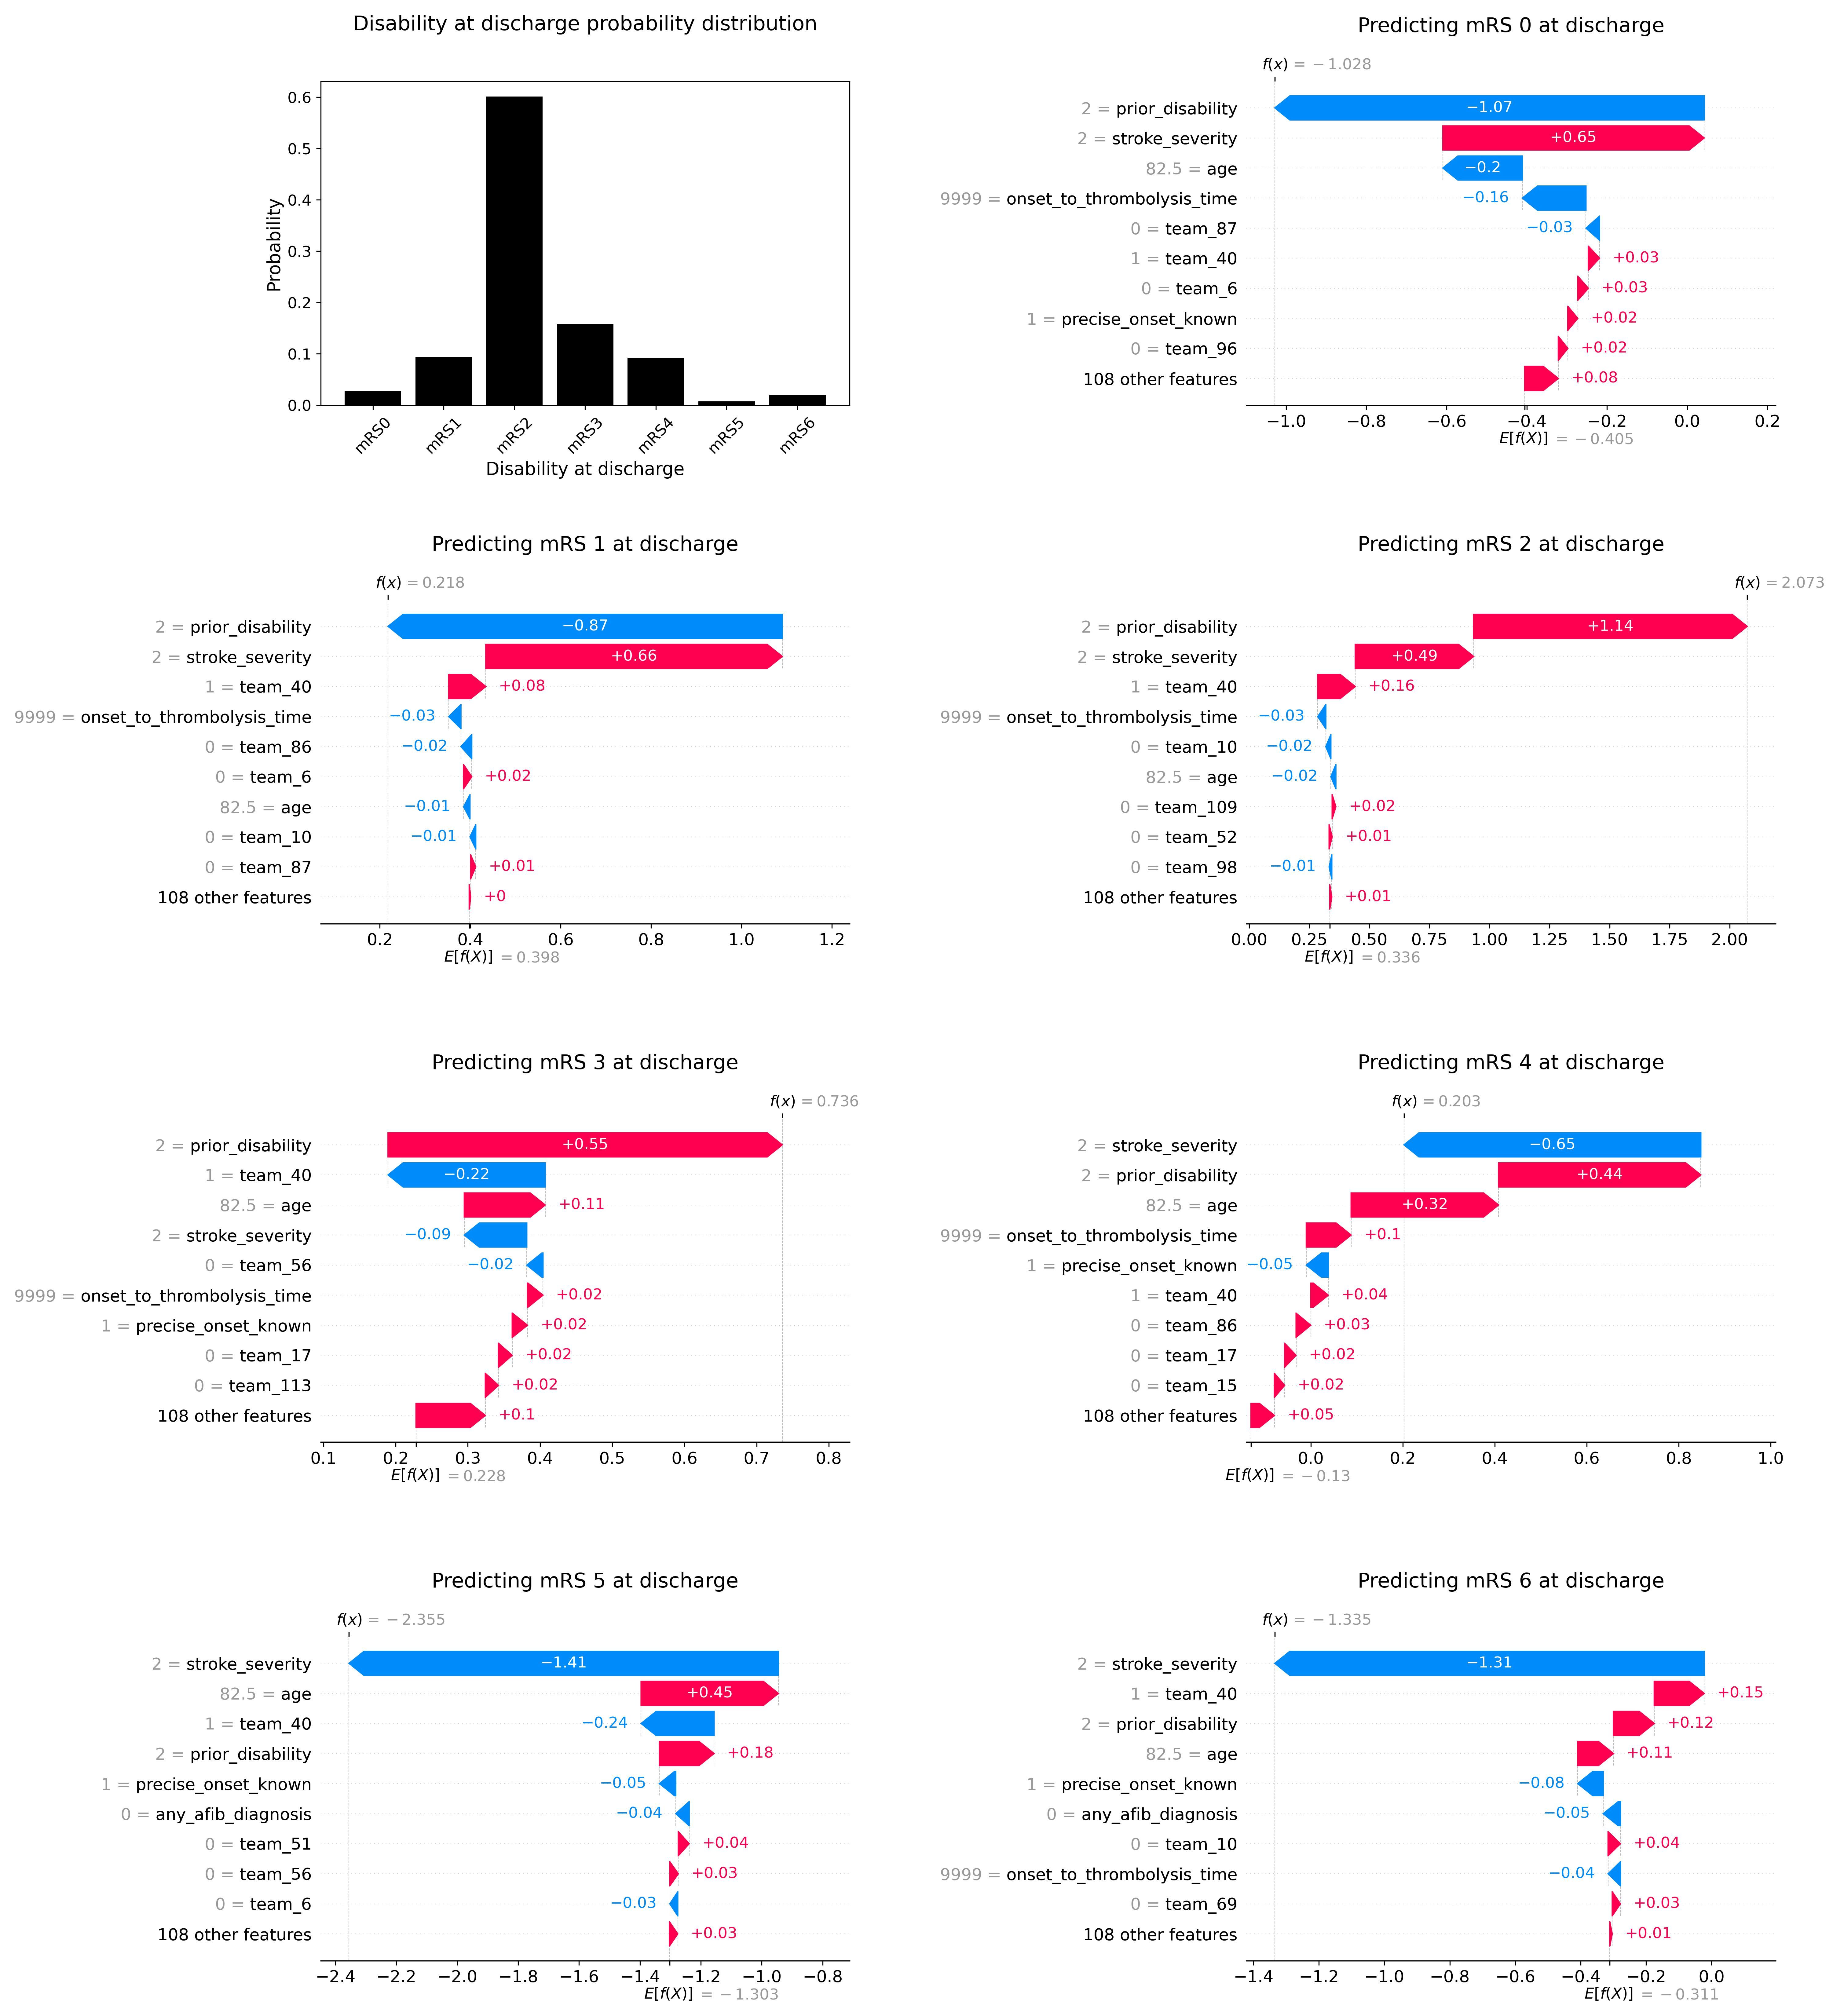
\includegraphics[width=1\linewidth]
{./images/042_xgb_7_features_5fold_probability_distribution_with_individual_waterfall_plots.jpg}}
  \caption{An example prediction for an individual patient (discharged mRS 2) showing the predicted probability of being discharged at each mRS level and waterfall plots showing the influence of each feature on the predicted likelihood of a single patient having each level of mRS at discharge. Each waterfall plot shows the SHAP base value, $E[f(X)$] (which is the same for all patient predictions for that mRS level), and the SHAP values for each of the input feature values. The sum of base and features SHAP values equates to the overall log likelihood for the patient being that mRS score at discharge, $f(x)$.}
  \label{fig:results_waterfall}
\end{figure}

%%%%%%%%%%%%%%%%%%%%%% POPULATION SHAP %%%%%%%%%%%%%%%%%%%%%%%%%%%%

\subsection{Influences on best and worst outcomes across a patient cohort}

In order to understand general characteristics affecting outcomes, we have shown how patient feature values, and stroke team attended, affected the likelihood of having the best (mRS 0) or worst (mRS 6) outcomes (figure \ref{fig:shap_outcome_model}) across 15,680 test patients (which were not used to train the model). Feature values that contributed to the best outcome on discharge (mRS 0) were no prior disability, milder stroke, earlier thrombolysis, younger, no atrial fibrillation diagnosis, and precisely known stroke onset time. Feature values that contributed to the worst outcome on discharge (mRS 6) were higher prior disability, more severe stroke, later or no thrombolysis, older, diagnosis of atrial fibrillation, and an imprecisely known onset time. The hospital attended also affected outcome predictions, with a  larger contribution from the attended hospital contribution for mRS 0, rather than mRS 6, at discharge. 


\begin{figure}
    \centering
    \begin{subfigure}{.5\textwidth}
      \centering
      \captionsetup{width=.9\linewidth}
      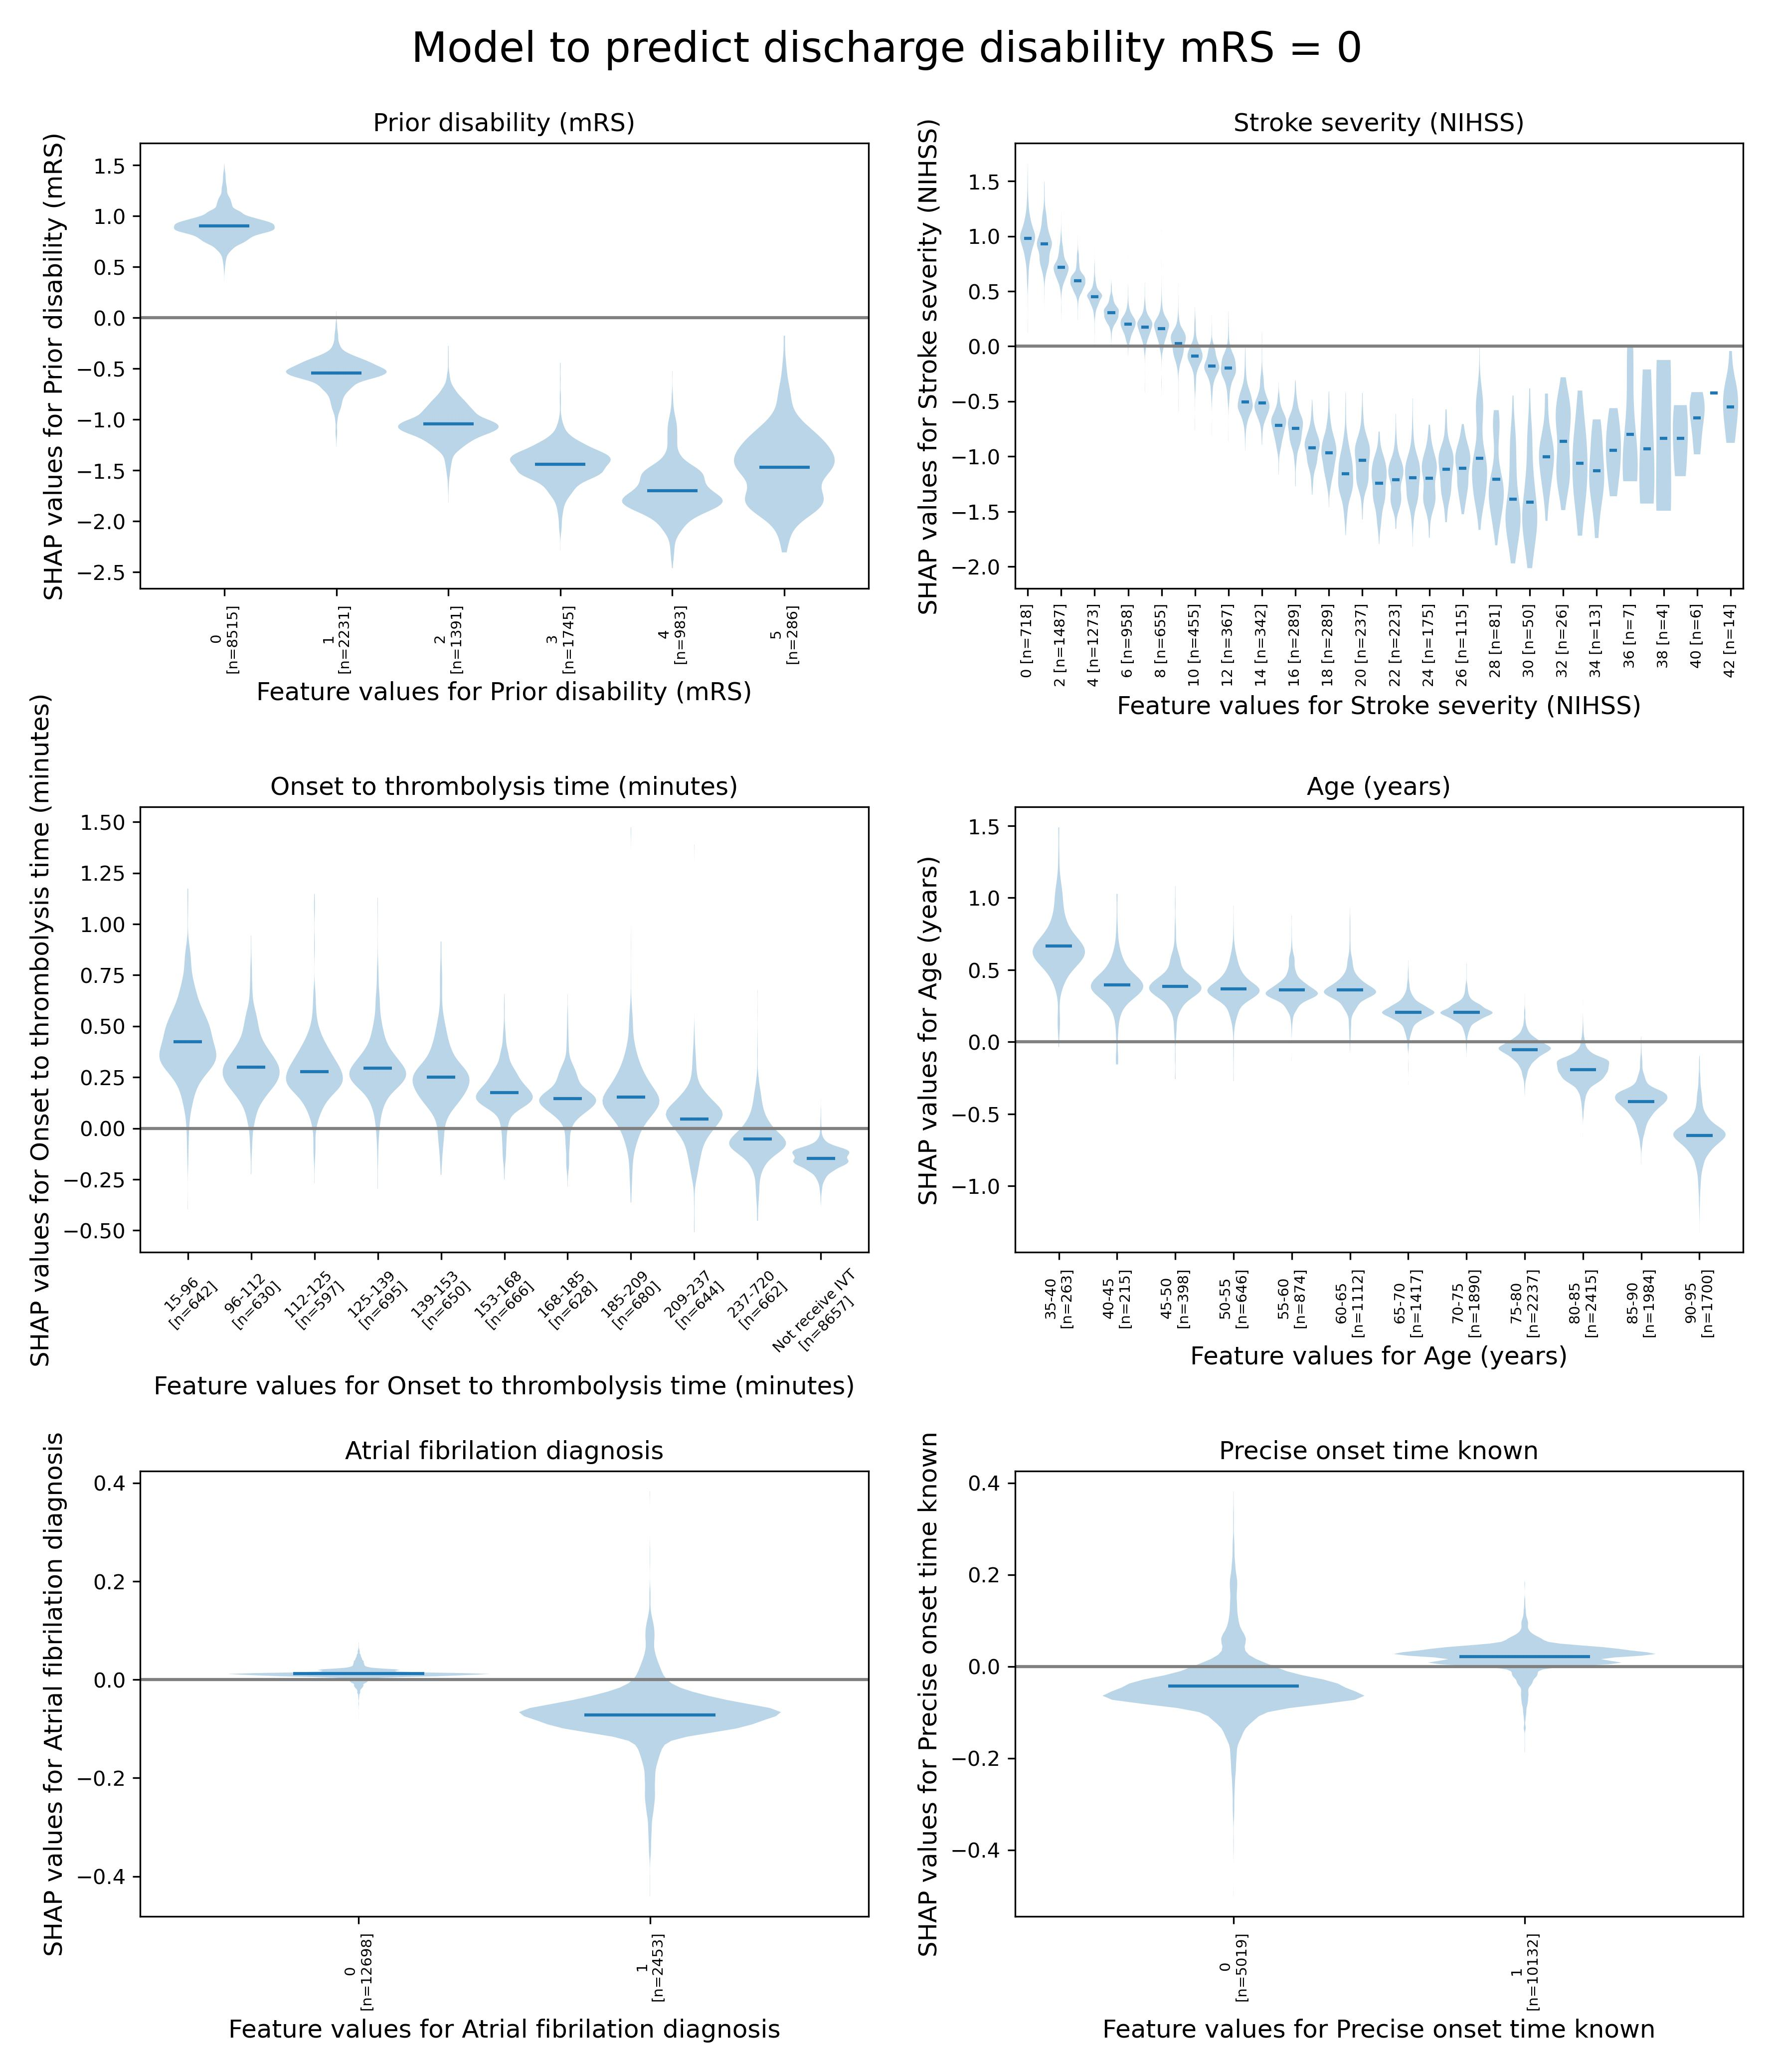
\includegraphics[trim={0 0 0 1.2cm}, clip, width=0.95\linewidth]      {./images/053_xgb_7_features_1fold_thrombolysis_shap_violin_all_features_for_mRS0}\\
      %{./images/053_xgb_7_features_1fold_999999_thrombolysis_shap_violin_all_features_for_mRS0}\\
%      \caption{SHAP values for the likelihood of no disability on discharge (mRS 0)}
%      \label{fig:mrs_violin}
    \end{subfigure}%ults
    \begin{subfigure}{.5\textwidth}
      \centering
      \captionsetup{width=.9\linewidth}
      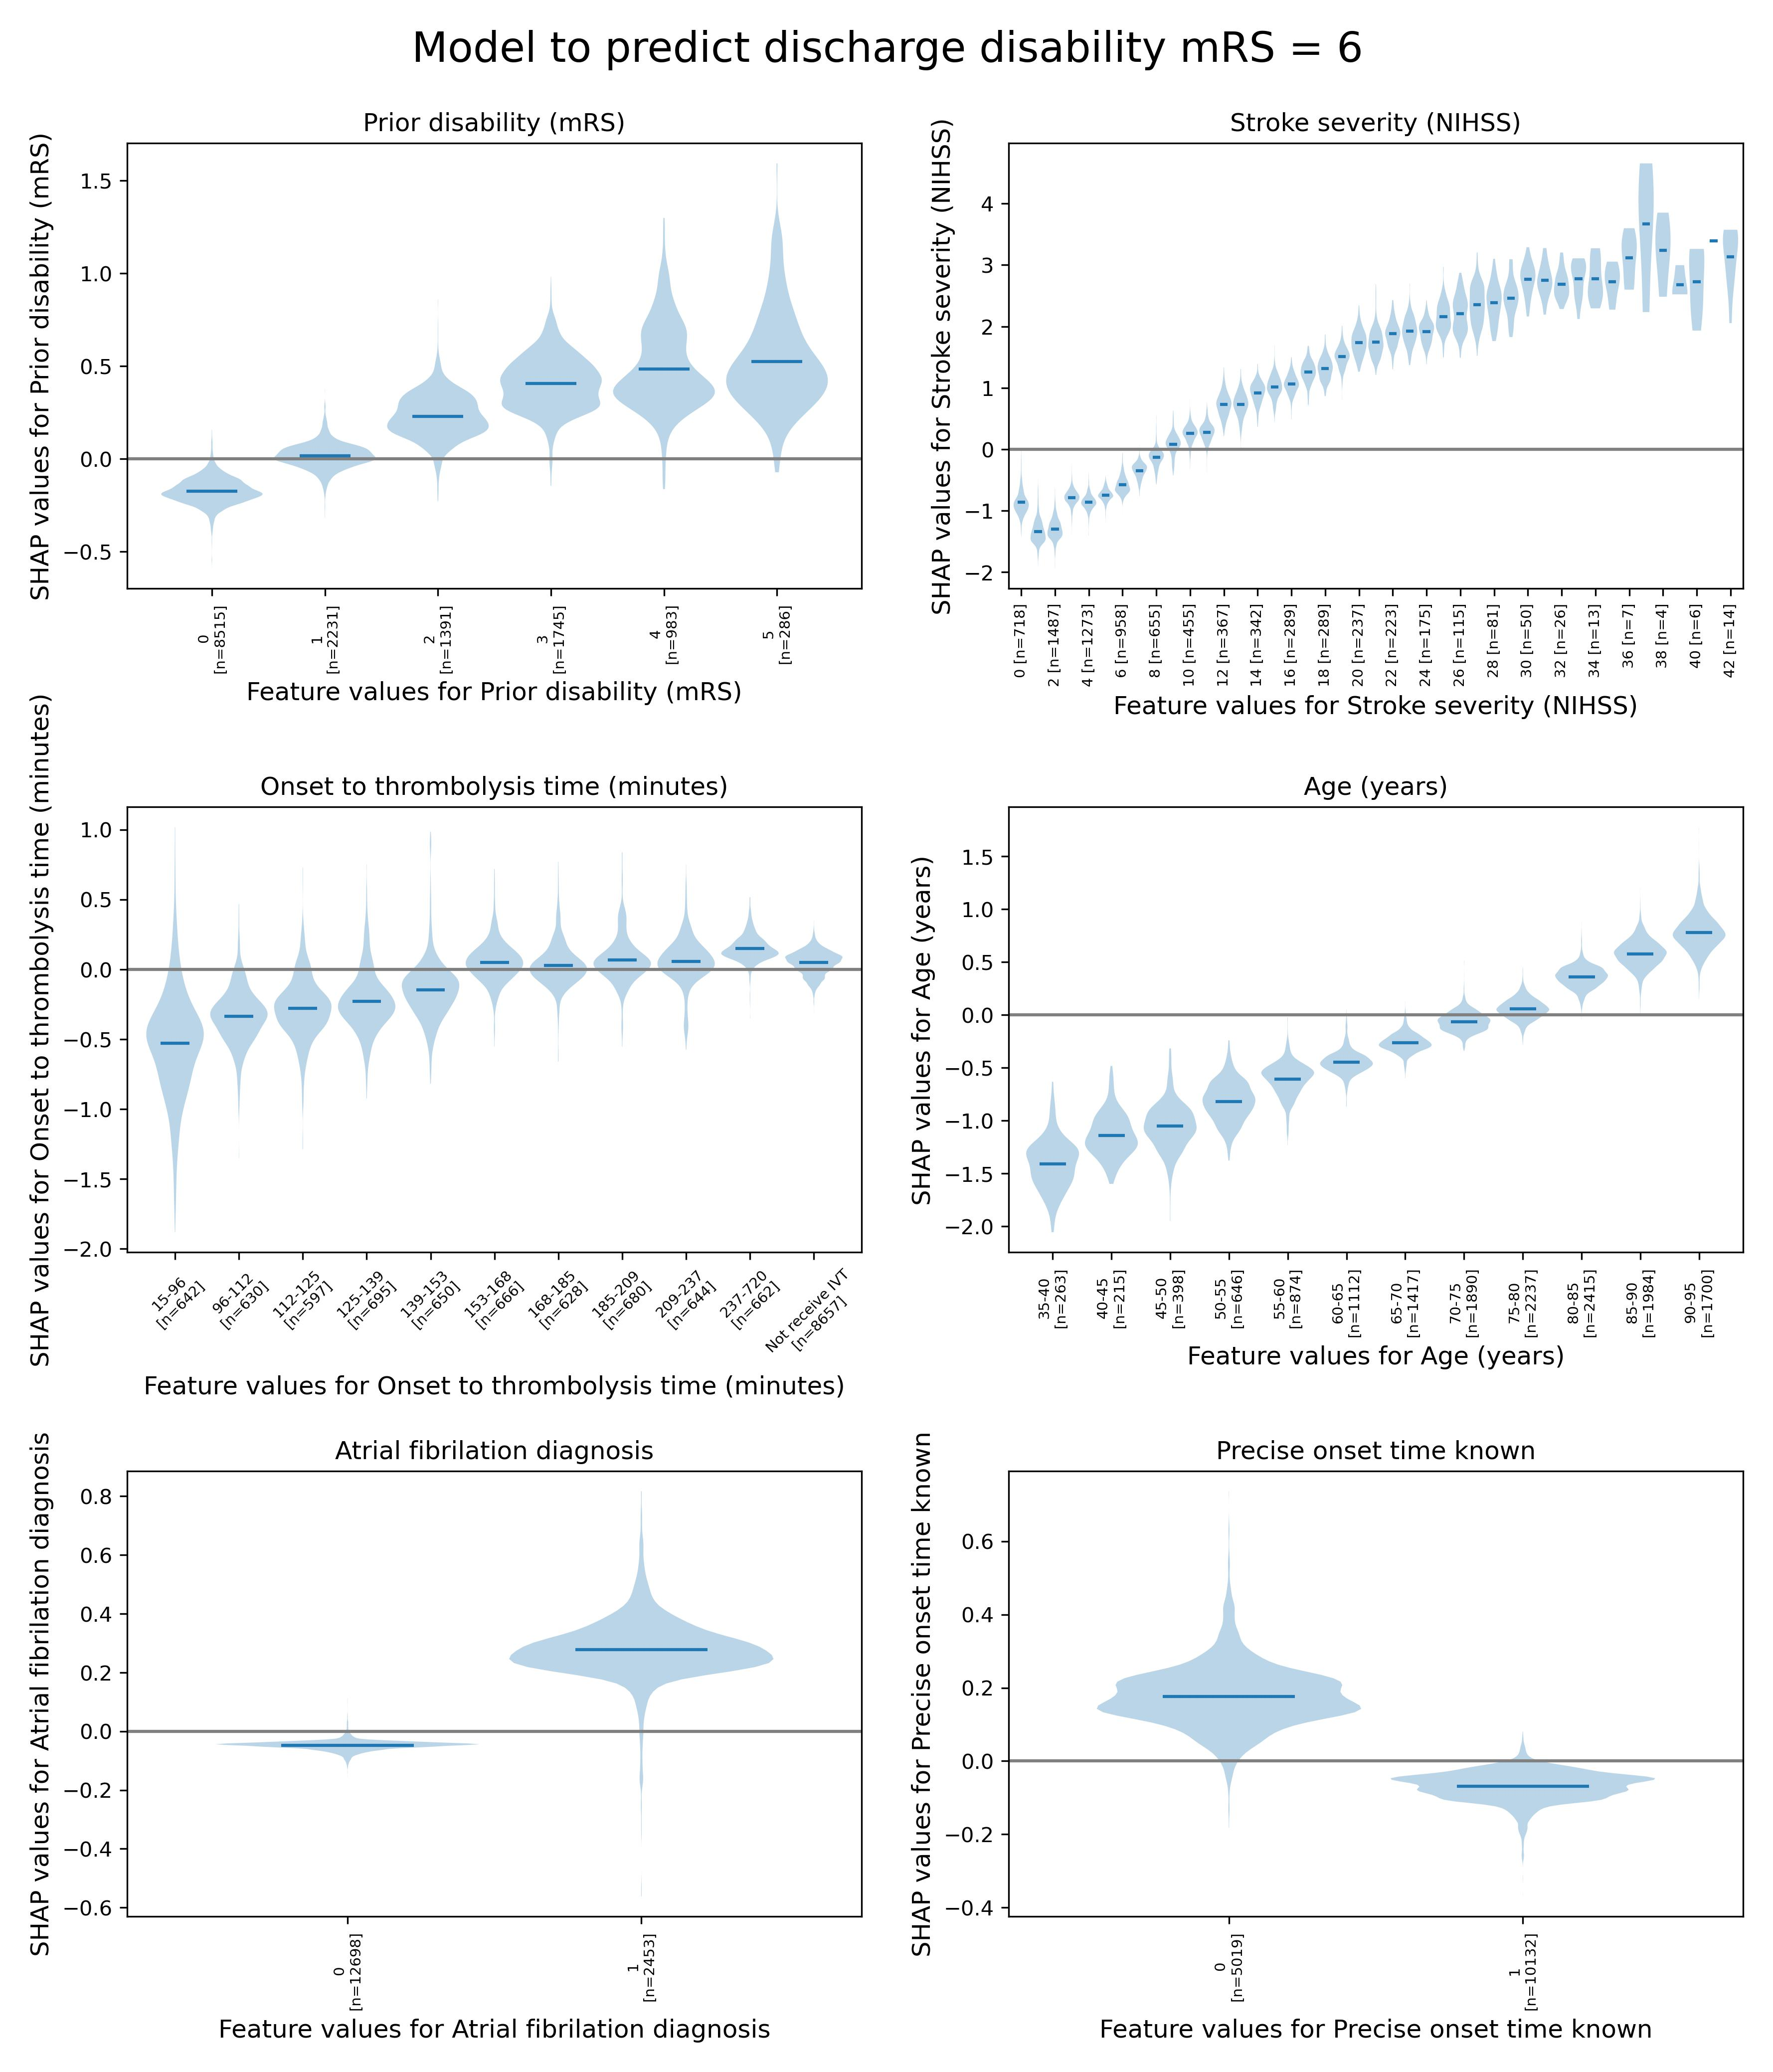
\includegraphics[trim={0 0 0 1.2cm}, clip, width=0.95\linewidth]      {./images/053_xgb_7_features_1fold_thrombolysis_shap_violin_all_features_for_mRS6}\\%{./images/053_predict_mrs6_split_by_ss.png}\\
      %{./images/053_xgb_7_features_1fold_999999_thrombolysis_shap_violin_all_features_for_mRS6}\\%{./images/053_predict_mrs6_split_by_ss.png}\\
%        \caption{Predict the likelihood of death on discharge (mRS 6)}
%        \label{fig:mrs6_violin_split}
    \end{subfigure}
    \hfill
    \begin{subfigure}{.5\textwidth}
      \centering
      \captionsetup{width=.9\linewidth}
      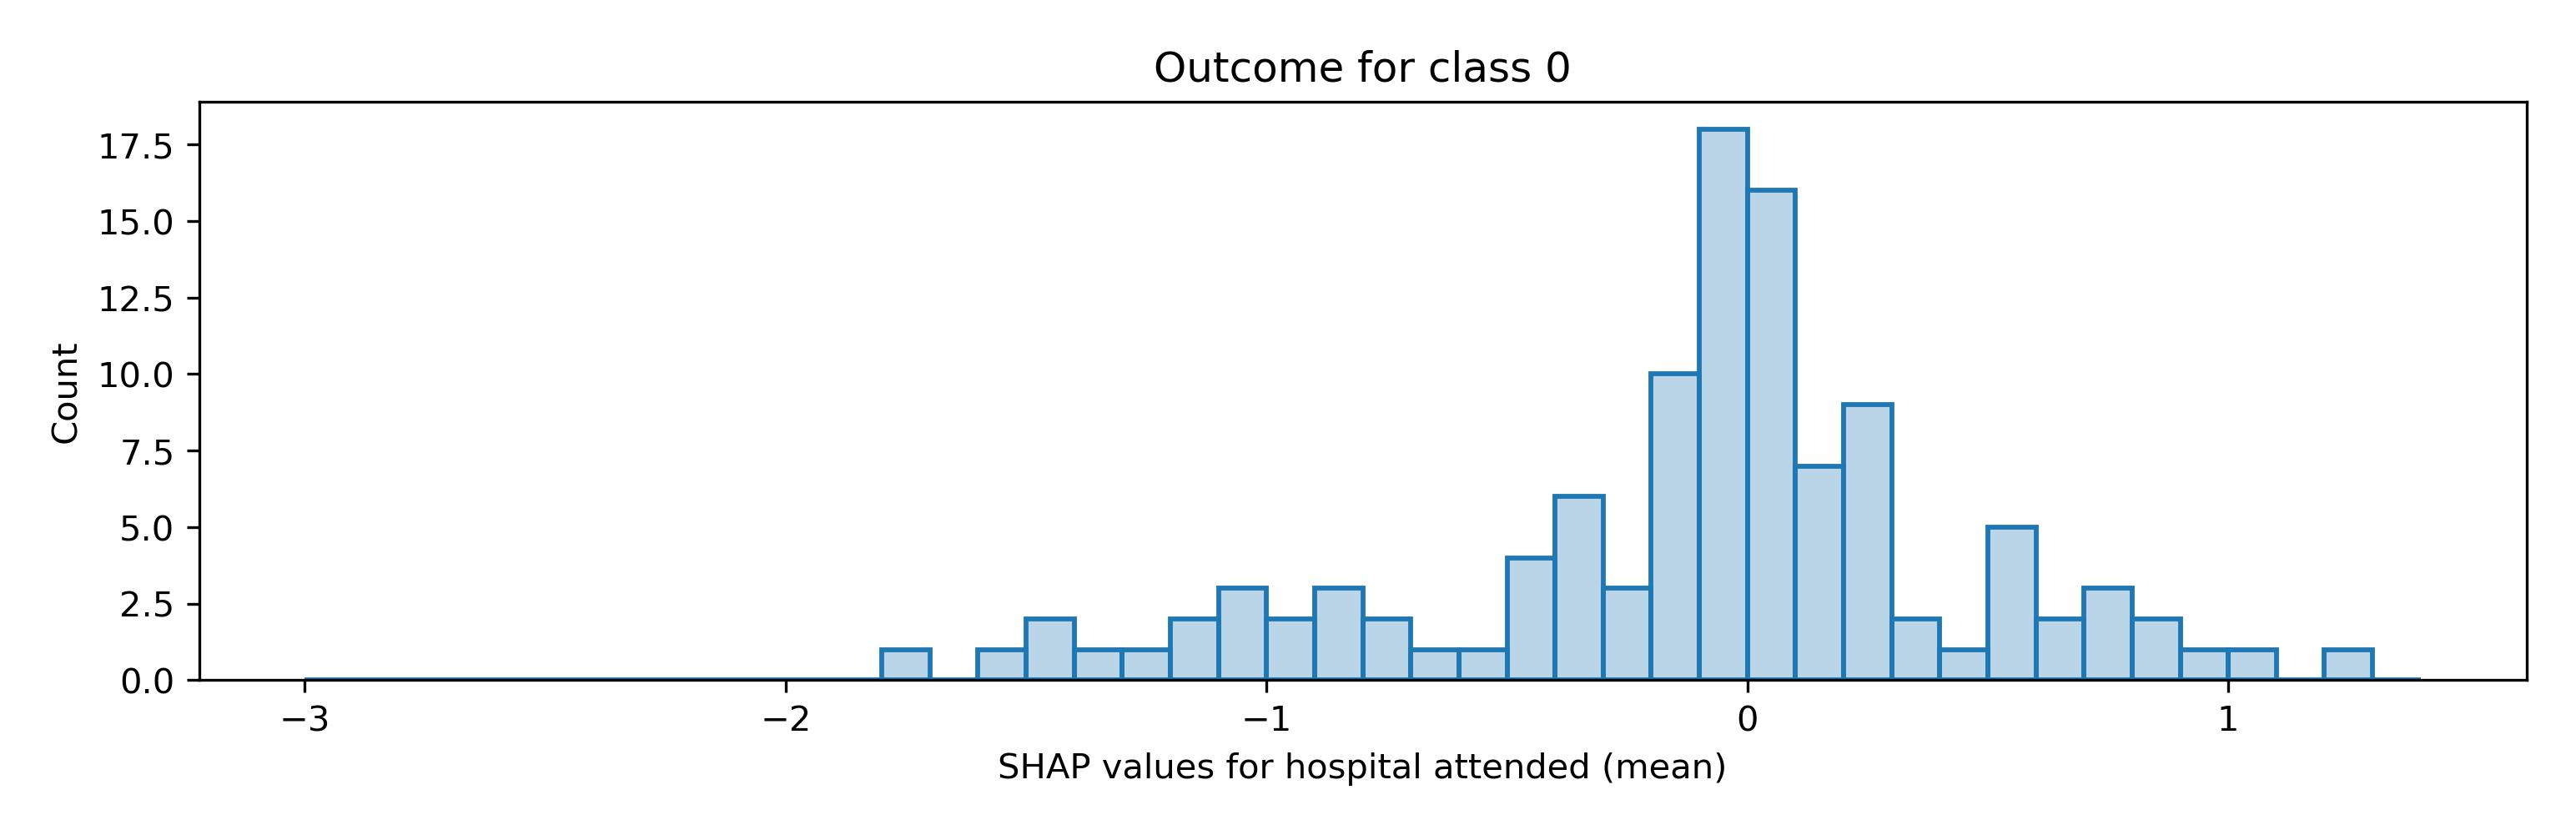
\includegraphics[trim={0 0 0 1cm}, clip, width=1\linewidth]    {./images/053_xgb_7_features_1fold_hosp_shap_hist_mrs0}\\%{./images/053_xgb_7_features_1fold_999999_hosp_shap_hist_mrs0}\\
      \caption{\footnotesize{SHAP values for the likelihood of no disability on discharge (mRS 0). Base SHAP value = -0.405}}
      \label{fig:mrs0_violin}
    \end{subfigure}%ults
    \begin{subfigure}{.5\textwidth}
      \centering
      \captionsetup{width=.9\linewidth}
      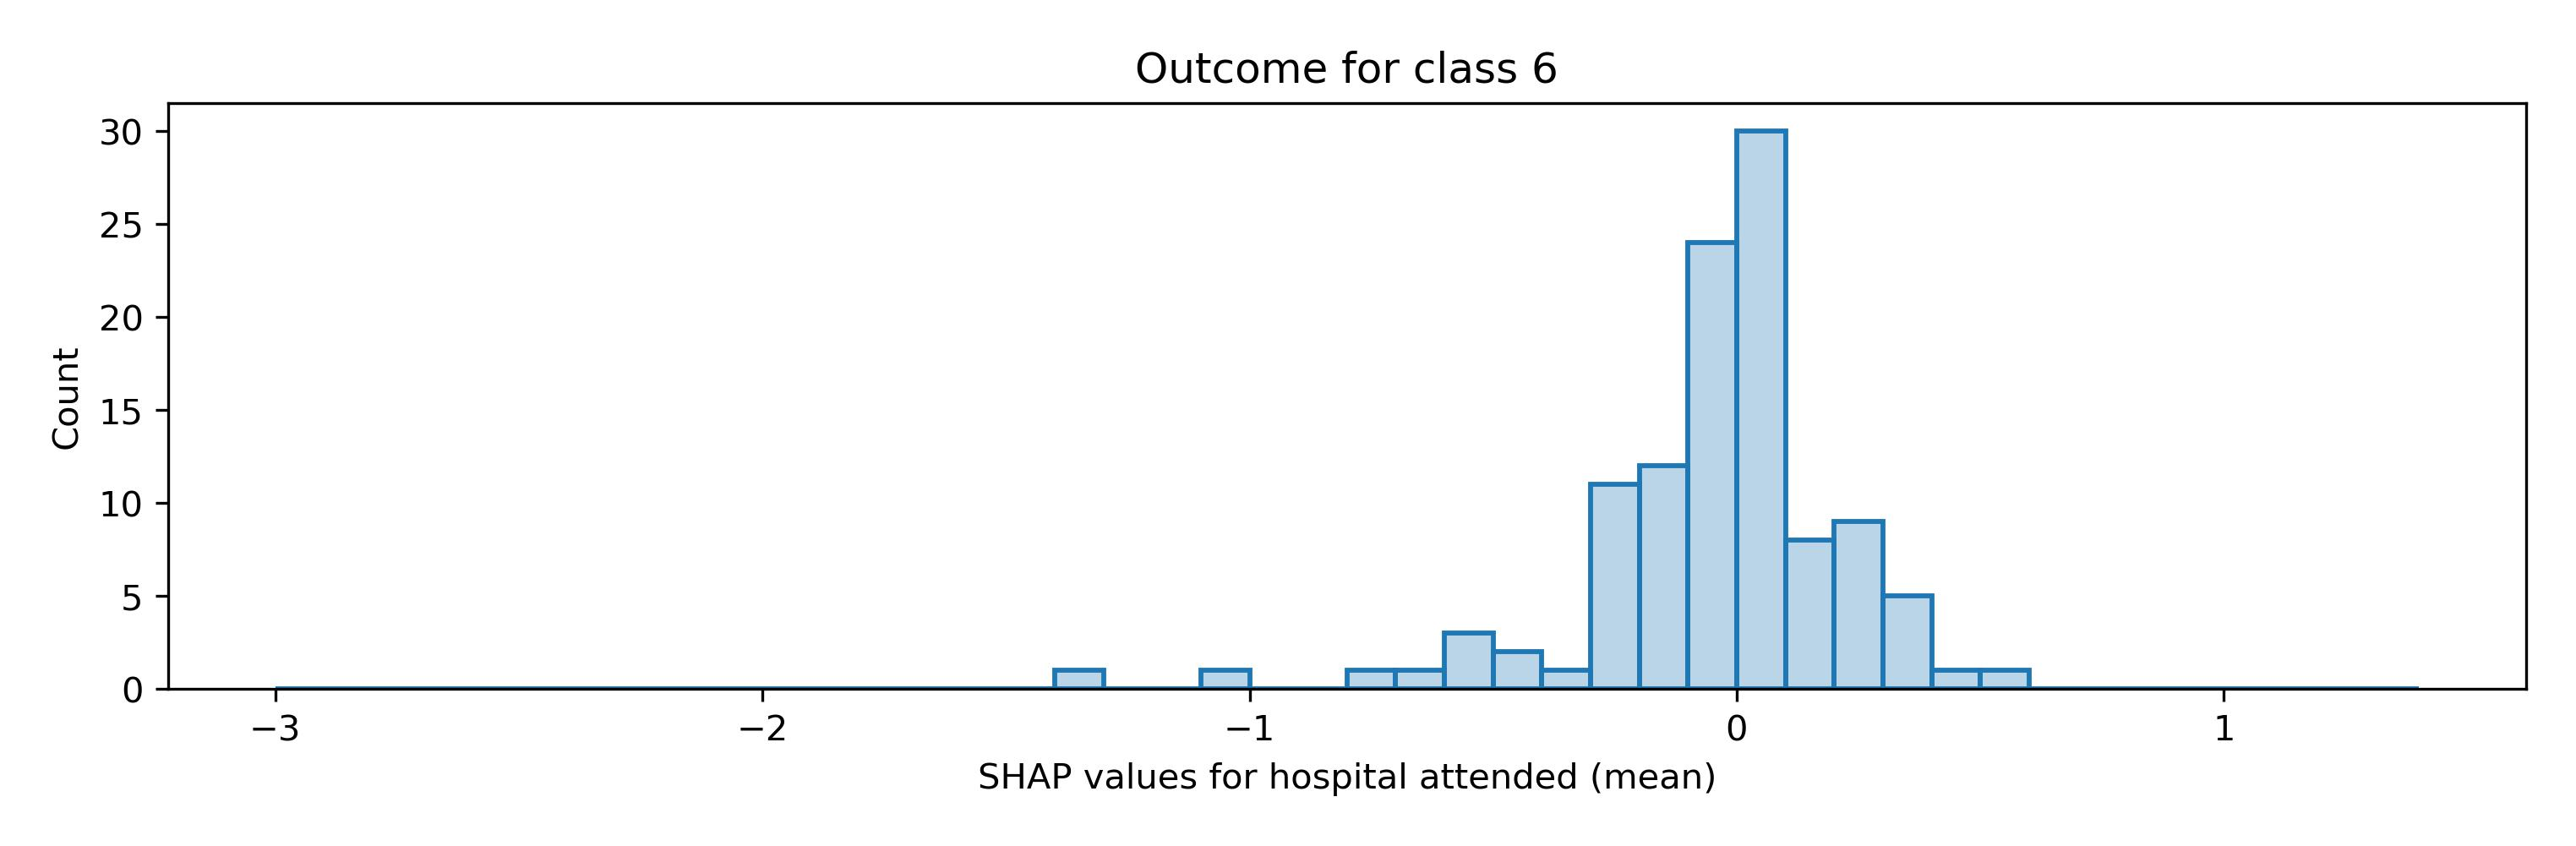
\includegraphics[trim={0 0 0 1cm}, clip, width=1\linewidth]
        {./images/053_xgb_7_features_1fold_hosp_shap_hist_mrs6}\\
%        {./images/053_xgb_7_features_1fold_999999_hosp_shap_hist_mrs6}\\
      \caption{\footnotesize{SHAP values for the likelihood of death at discharge (mRS 6). Base SHAP value = -0.311}}
      \label{fig:mrs6_violin}
    \end{subfigure}
  \caption{Plots showing the relationship between SHAP values and feature values for best or worse possible outcomes. Left: Predicting the likelihood of having no disability at discharge (mRS 0). Right: Predicting the likelihood of being dead at discharge (mRS 6). Top: Violin plots showing the relationship between SHAP values and feature values. The horizontal line shows the median SHAP value. Bottom: Histogram showing the frequency of the mean SHAP value for the hospital attended.}
    \label{fig:shap_outcome_model}
\end{figure}

%%%%%%%%%%%%%%%%%%%%%% PROTOTYPE PATIENTS %%%%%%%%%%%%%%%%%%%%%%%%%%%%


\subsection{Prototype patients and the effect of thrombolysis on outcomes}

In order to further understand and illustrate the effect of thrombolysis on outcomes we created eight \textit{prototype} patients. The base patient in these patients was a patient that would generally be considered an ideal candidate for thrombolysis. We then altered each feature of that patient in a controlled way. This gave the following patients:

\begin{enumerate}
    \item \textit{Ideal}: No prior disability (mRS 0), age 72.5, no atrial fibrillation diagnosis, NIHSS 15, precise onset time, onset to thrombolysis time 2 hours. The patient attended a hospital with the most neutral contribution towards use of thrombolysis.
    \item \textit{Mild stroke}: As \textit{Ideal} but NIHSS 3
    \item \textit{Severe stroke}: As \textit{Ideal} but NIHSS 25
    \item \textit{Prior disability 3}: As \textit{Ideal} but prior disability mRS 3
    \item \textit{Prior disability 4}:  As \textit{Ideal} but prior disability mRS 4
    \item \textit{Atrial fibrillation diagnosis}: As \textit{Ideal} but with an atrial fibrillation diagnosis
    \item \textit{Older}: As \textit{Ideal} but age 87.5
    \item \textit{Imprecise onset time}: As \textit{Ideal} but imprecise onset time
\end{enumerate}

We predicted mRS distributions for each patient with and without thrombolysis. We also classified whether the patient would likely have both an improvement in the probability-weighted disability at discharge and a reduction in probability of having the worst outcomes of mRS 5-6. Results are shown in figure \ref{fig:counterfactual_bar_plot}. Thrombolysis was predicted to improve outcomes across all patients, but the benefit was significantly lower with mild stroke.

\begin{figure}
\centering
 {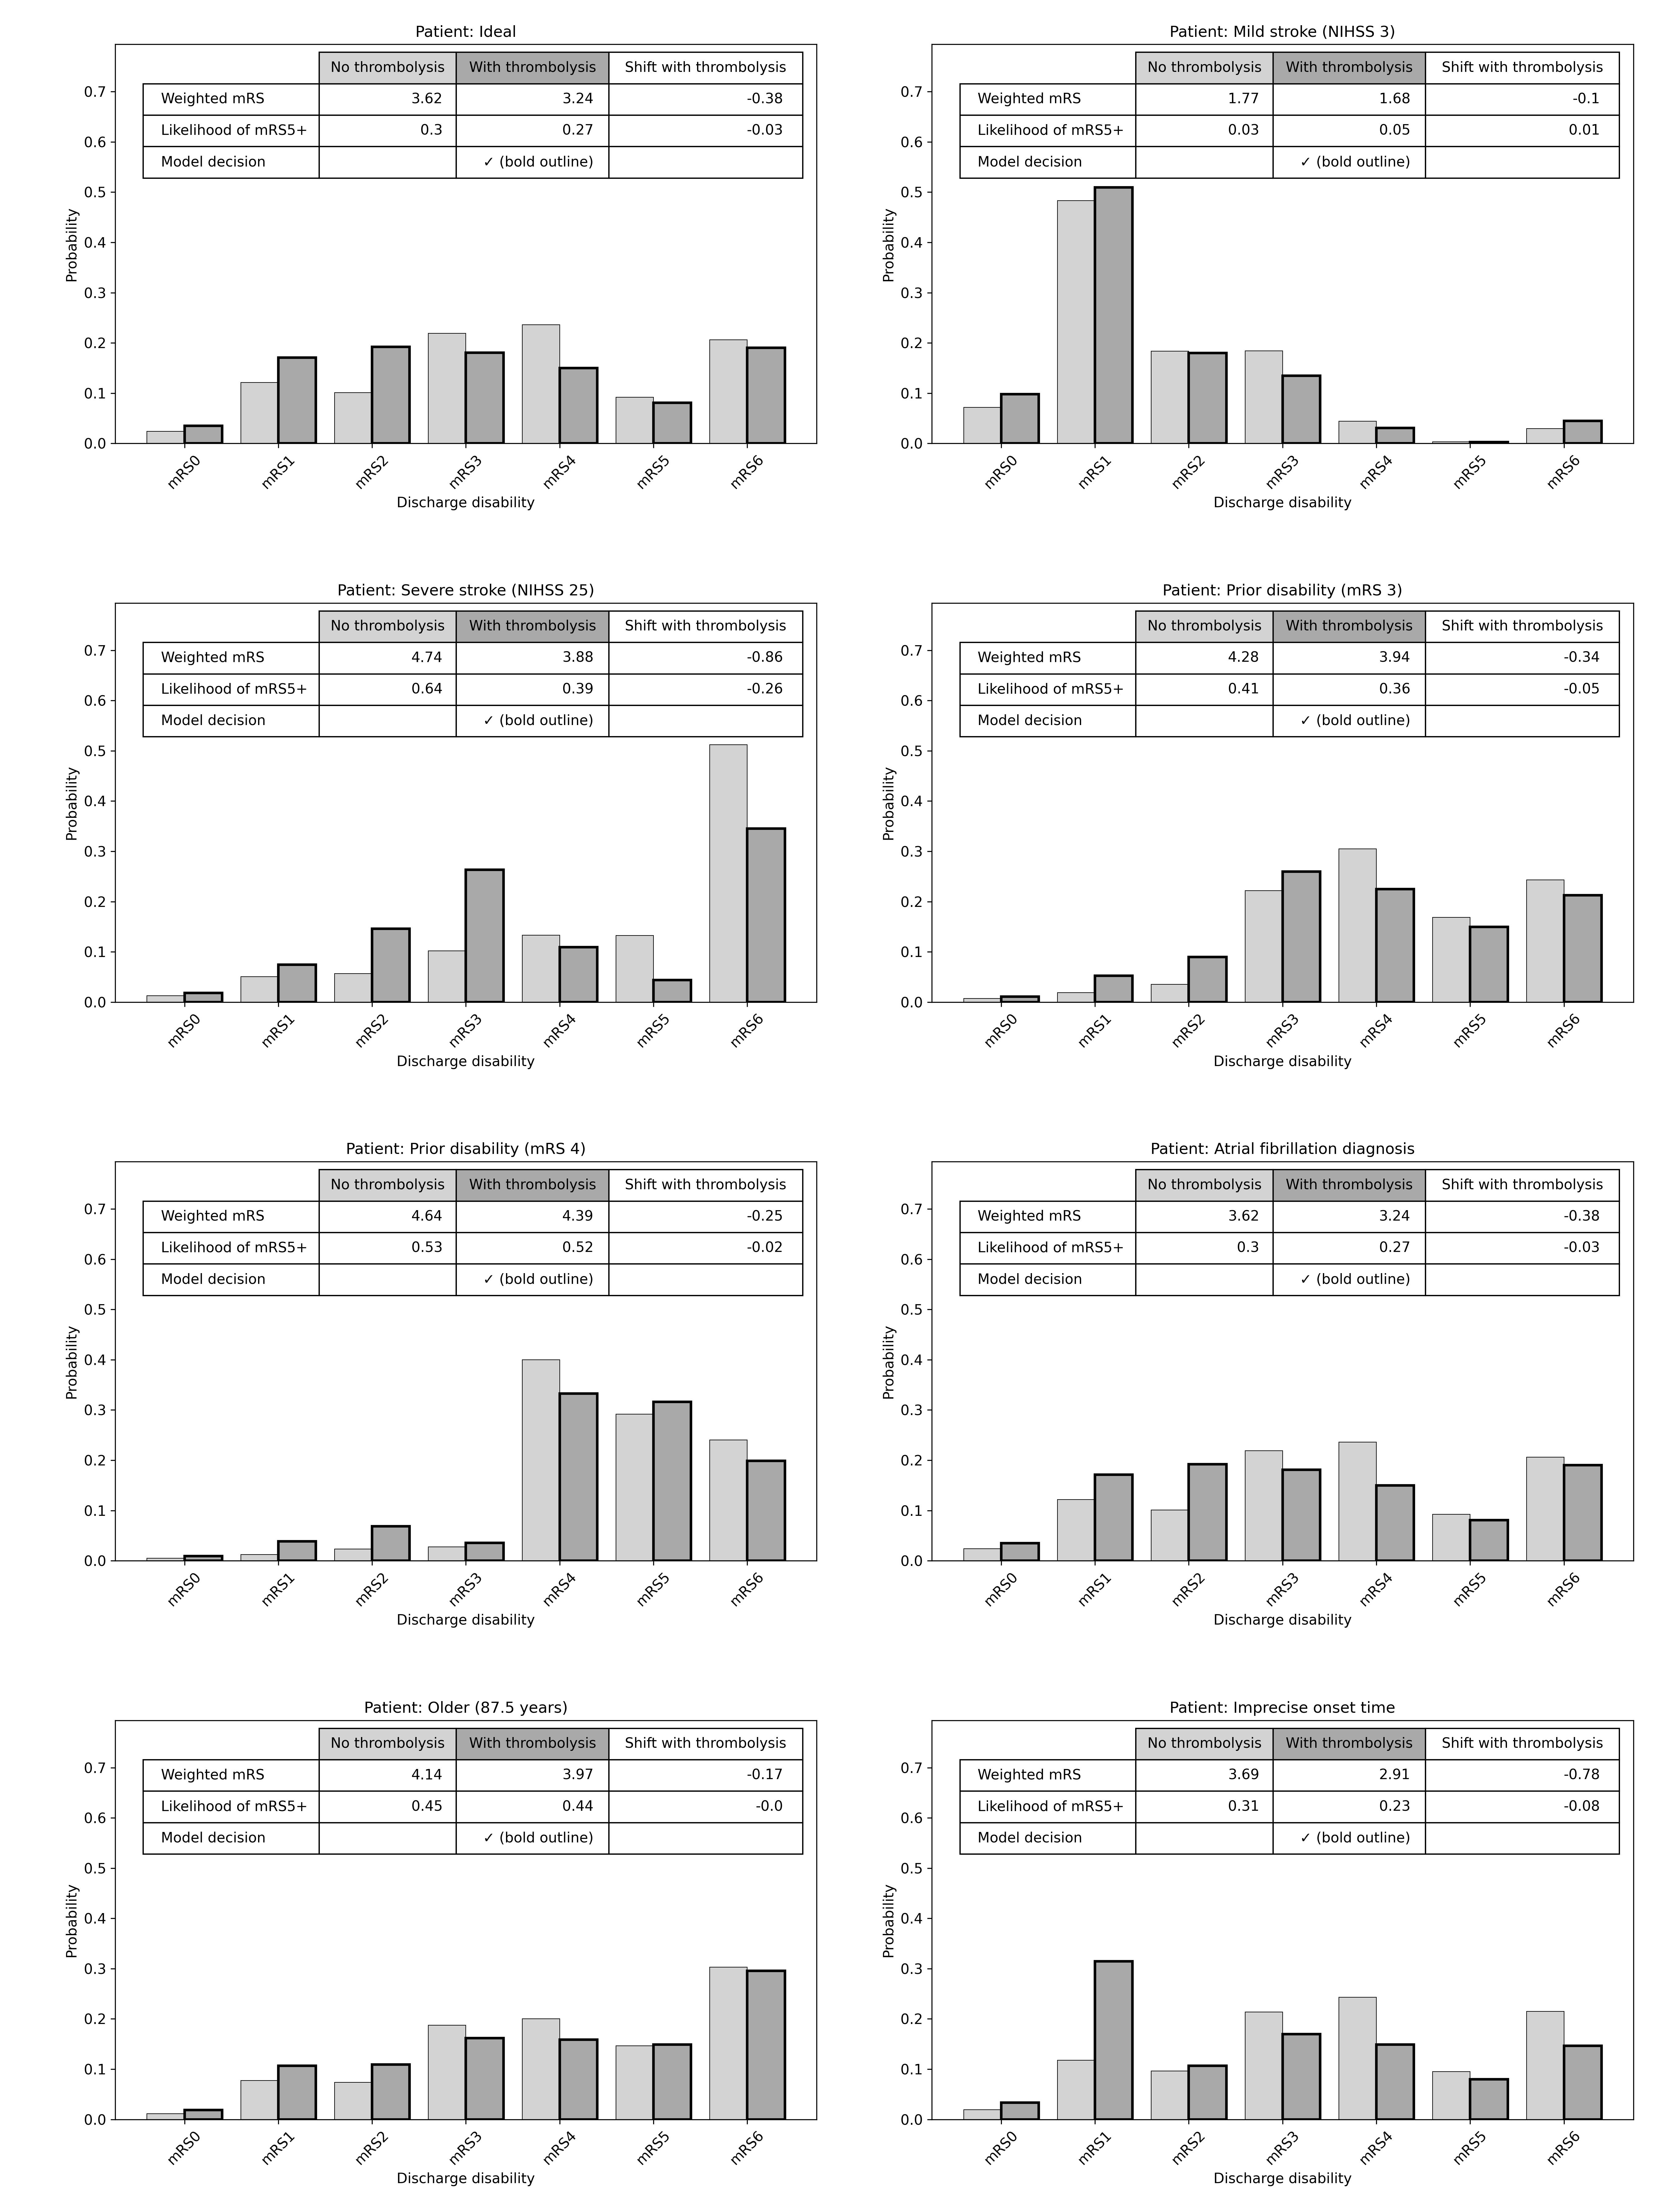
\includegraphics[width = 6.1in]{./images/060_xgb_mrs_distributions_bar_plot_table_bw.jpg}}\\%{./images/060_xgb_mrs_distributions_999999_bar_plot.jpg}}\\%060_bar_plot.png}}\\
 \caption{Probability distribution of disability at discharge (as mRS score) for eight defined patients. i. \textit{Ideal}: No prior disability (mRS 0), age 72.5, no afib diagnosis, NIHSS 15, precise onset time, onset to treatment 2 hours, attended stroke team with most neutral contribution towards use of thrombolysis. ii. \textit{Mild stroke}: As \textit{Ideal} but NIHSS 3. iii. \textit{Severe stroke}: As \textit{Ideal} but NIHSS 25. iv. \textit{Prior disability (mRS3)}: As \textit{Ideal} but prior disability mRS 3. v. \textit{Prior disability (mRS 4)}:  As \textit{Ideal} but prior disability mRS 4. vi. \textit{Atrial fibrillation diagnosis}: As \textit{Ideal} but with an atrial fibrillation diagnosis. vii. \textit{Older (87.5 years)}: As \textit{Ideal} but age 87.5. viii. \textit{Imprecise onset time}: As \textit{Ideal} but imprecise onset time. Inset table shows the values for the two criteria that defines whether a patient has a better outcome with thrombolysis, and the treatment decision that this method would decide.}
 \label{fig:counterfactual_bar_plot}
\end{figure}

%%%%%%%%%%%%%%%%%%%%%% SCATTER PLOT %%%%%%%%%%%%%%%%%%%%%%%%%%%%

\subsection{Comparing actual use of thrombolysis and predicted benefit from thrombolysis}

In the first k-fold test set of 15,680 patients, 44\% received thrombolysis. For each patient we predicted outcomes with and without thrombolysis. Figure \ref{fig:scatter_all} shows the expected shift in probability-weighted mRS at discharge, and the change in probability of being discharged with mRS 5-6, due to thrombolysis, separated by whether the patient actually received thrombolysis or not. Overall, 60\% of patients were predicted to benefit from thrombolysis. Of those who did receive thrombolysis, 73\% were predicted to have both a better average disability likelihood and a reduction in probability of being mRS 5-6. 9\% were predicted to have both a worse average disability likelihood and an increase in probability of being mRS 5-6. 18\% were predicted to have either, but not both, an improved average disability likelihood or a reduction in probability of being mRS 5-6. Of those who did not receive thrombolysis, 49\% were predicted to have both a better average disability likelihood and a reduction in probability of being mRS 5-6. 26\% were predicted to have both a worse average disability likelihood and an increase in probability of being mRS 5-6. 25\% were predicted to have either, but not both, an improved average disability likelihood or a reduction in probability of being mRS 5-6.

\begin{figure}
\centering
\begin{subfigure}{.7\textwidth}
  \centering
  \captionsetup{width=.9\linewidth}
  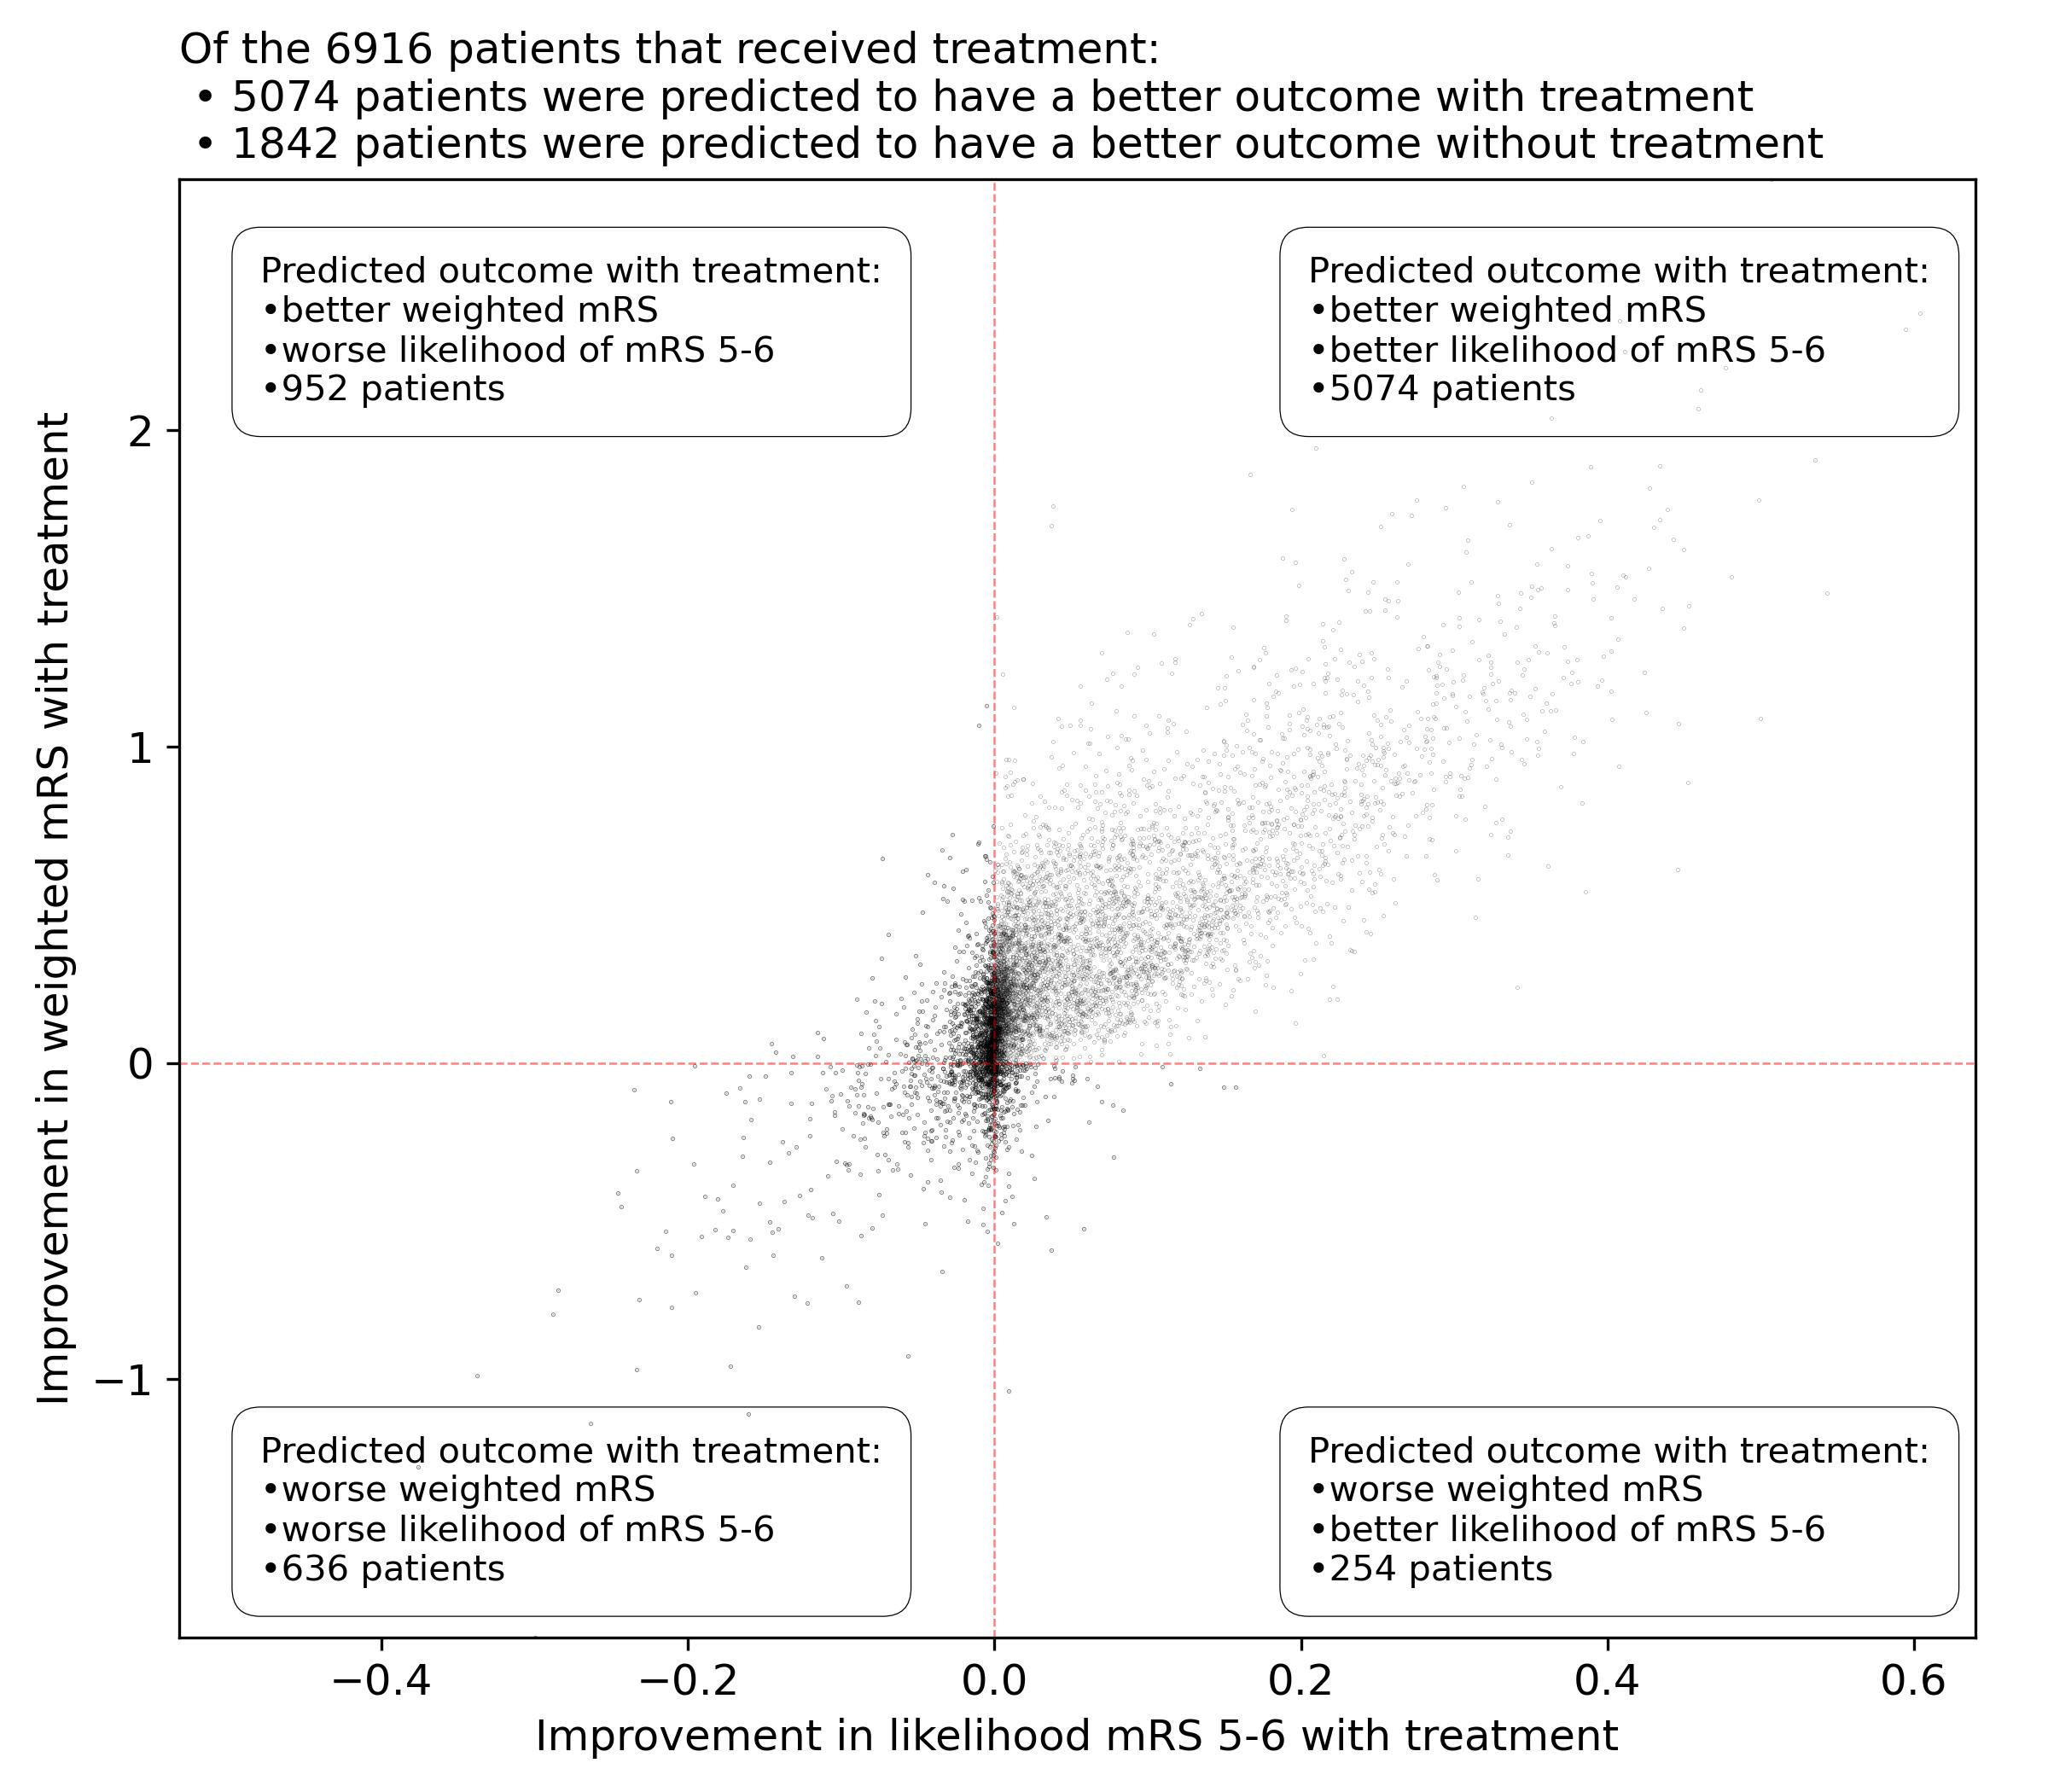
\includegraphics[trim={0 0 0 1.7cm}, clip, width=1\linewidth]{./images/210_xgb_all_data_multiclass_outcome_scatter_criteria_treated}%210_better_outcome_criteria_scatter_treated.png}
  \caption{\footnotesize{Patients who received thrombolysis  (n = 6,916)}}
  \label{fig:scatter_receive}
\end{subfigure}

\vspace{5mm}

\begin{subfigure}{.7\textwidth}
  \centering
  \captionsetup{width=.9\linewidth}
  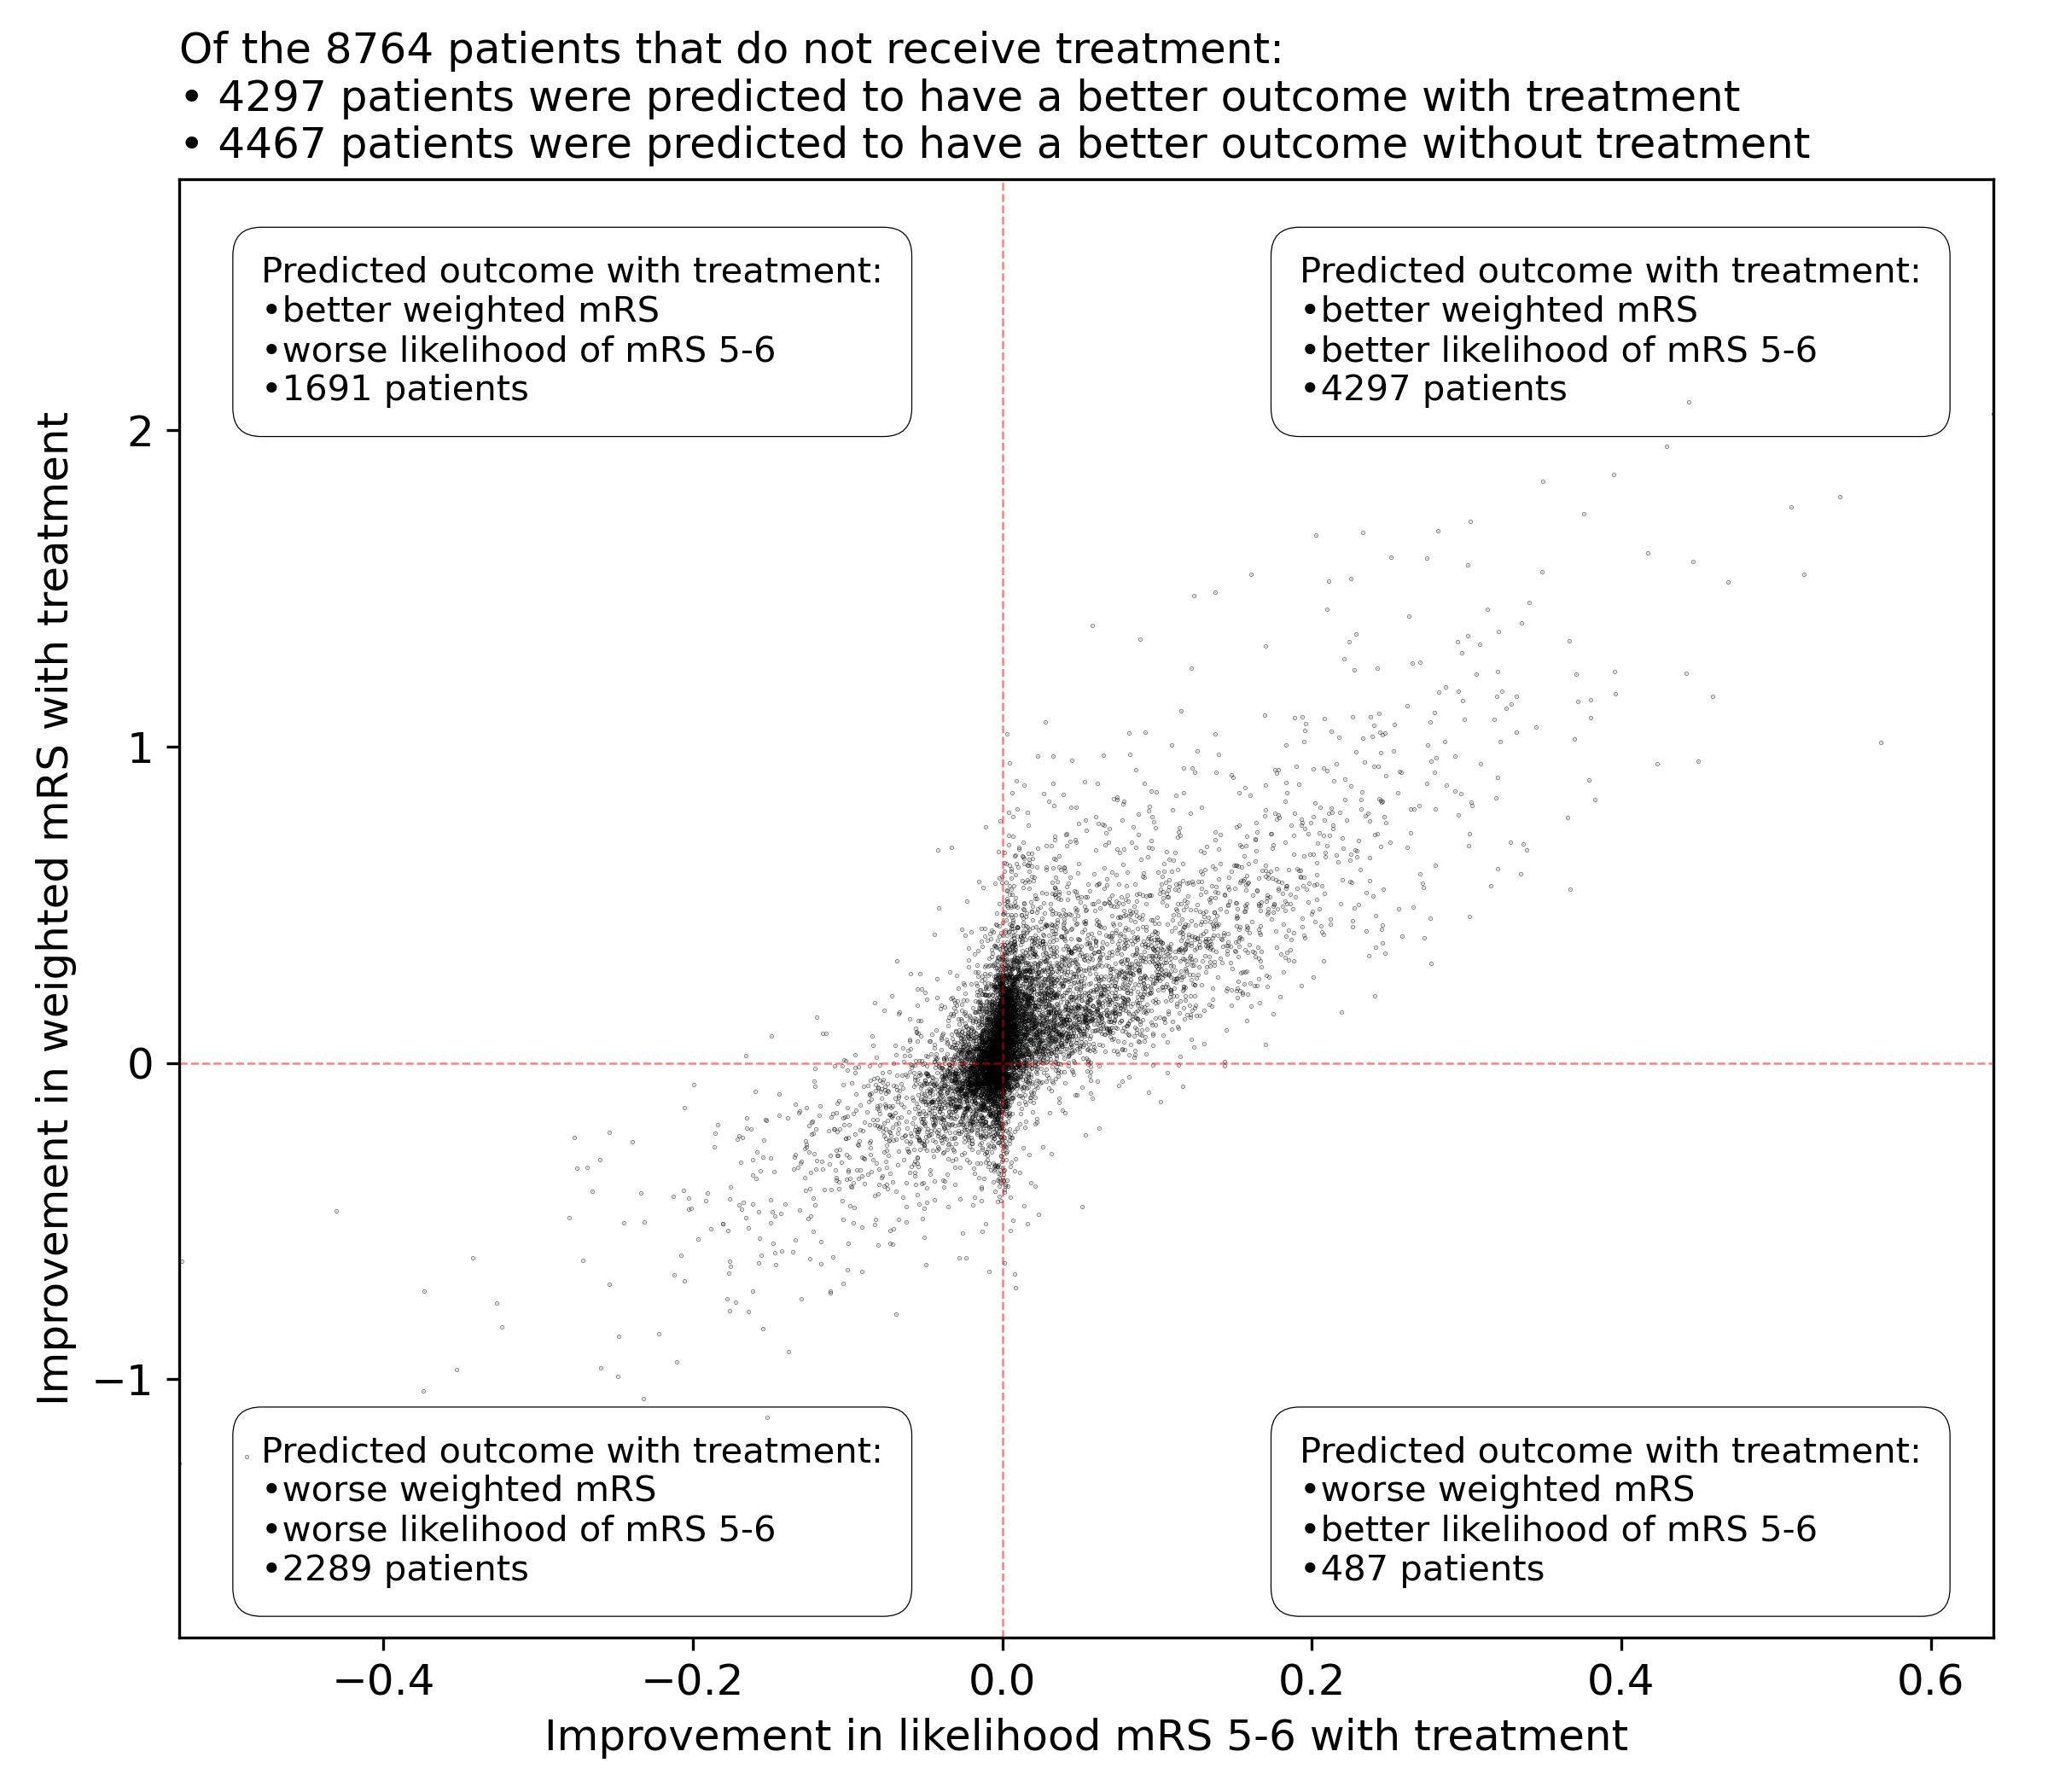
\includegraphics[trim={0 0 0 1.7cm}, clip, width=1\linewidth]{./images/210_xgb_all_data_multiclass_outcome_scatter_criteria_not_treated}%210_better_outcome_criteria_scatter_not_treated.png}
  \caption{\footnotesize{Patients who did not receive thrombolysis (n = 8,764)}}
  \label{fig:scatter_not_receive}
\end{subfigure}
  \caption{The predicted benefit or disbenefit of thrombolysis for each of 15,680 patients. Benefit is shown as both the expected improvement in probability-weighted disability (y-axis) and the improvement in likelihood of avoiding discharge with mRS 5-6. Both measures are expressed so that a positive value is better (a reduction in probability-weighted disability or a reduction in probability of discharge with mRS 5-6). (a) Patients who did actually receive thrombolysis (n = 6,916), (b) Patients who did not actually receive thrombolysis (n = 8,764).}
\label{fig:scatter_all}
\end{figure}

%%%%%%%%%%%%%%%%%%%%%% MISMATCH %%%%%%%%%%%%%%%%%%%%%%%%%%%%

\subsection{Patient characteristics that contribute to a mismatch between actual thrombolysis use and predicted best outcome}

Figure \ref{fig:decriptive_plots_2_cohorts} shows the distribution of feature values for two patient cohorts: (i) 1,842 patients that received thrombolysis but were predicted to not have a better outcome with thrombolysis, (ii) 4,297 that did not receive thrombolysis but were predicted to have a better outcome with thrombolysis.

When examining individual feature values in this way we did not identify any features that could be used in isolation to identify those patients who would benefit from thrombolysis but did not receive thrombolysis (or vice-versa). Patients who received thrombolysis but would likely not benefit from it have a range of feature values for each patient feature, as do those patients who did not receive thrombolysis but would benefit from it.

%./images/210_xgb_all_data_multiclass_outcome_999999_descriptive_plots_2_patient_cohorts
\begin{figure}
    \centering
    \captionsetup{width=1\linewidth}
    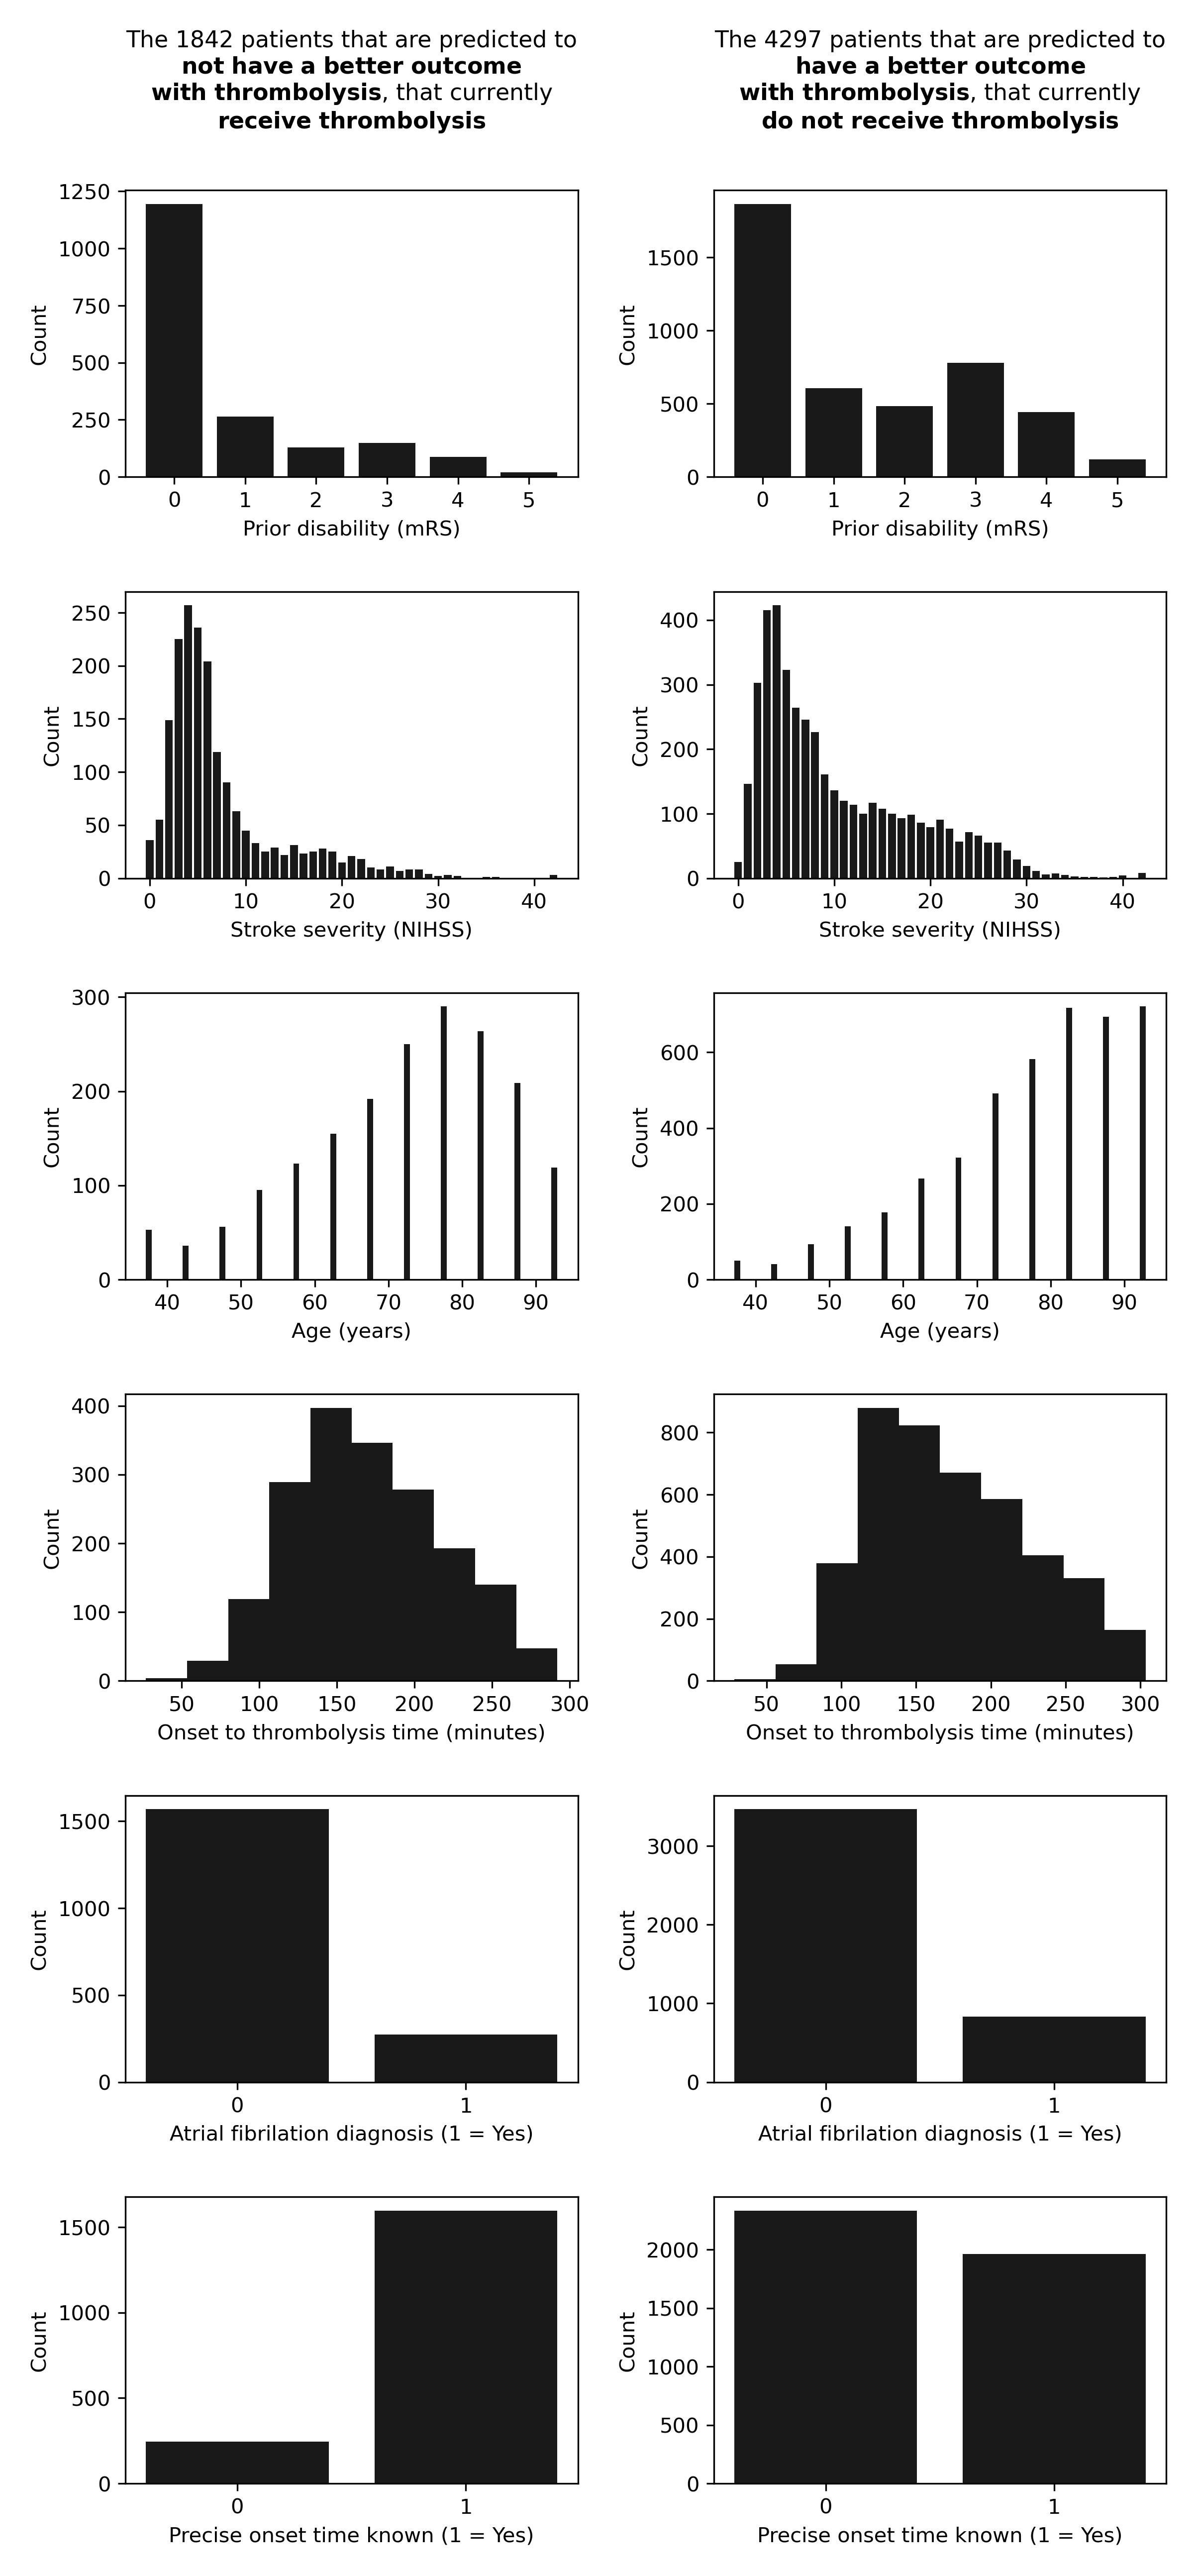
\includegraphics[width=0.6\linewidth]{./images/210_xgb_all_data_multiclass_outcome_descriptive_plots_2_patient_cohorts}\\
  \caption{Plots showing the frequency of feature values for patient cohorts where actual treatment decision differed from best predicted outcome. \textit{Left}: patients that were predicted to not have a better outcome with thrombolysis, but received thrombolysis. \textit{Right}: patients that were predicted to have a better outcome with thrombolysis, but did not receive thrombolysis.}
  \label{fig:decriptive_plots_2_cohorts}
\end{figure}

%%%%%%%%%%%%%%%%%%%%%% SENSITIVITY AND SPECIFICITY %%%%%%%%%%%%%%%%%%%%%%%%%%%%

\subsection{Hospital trade-off between maximising benefit from thrombolysis and minimising risk of harm from thrombolysis}

The XGBoost \textit{thrombolysis decision} model had an accuracy of 78.7\% and ROC-AUC of 0.86. Figure \ref{fig:hosp_shap_scatter} shows the trade-off between the individuals hospital sensitivity and specificity towards giving treatment. We found that those hospitals attaining a higher predicted \textit{sensitivity} of treatment (not missing patients who would benefit from treatment) also tended to have a lower \textit{specificity} (giving thrombolysis to patients who would likely not benefit from it).

%218_hosp_shap_scatter.png}}\\

\begin{figure}
    \centering
    {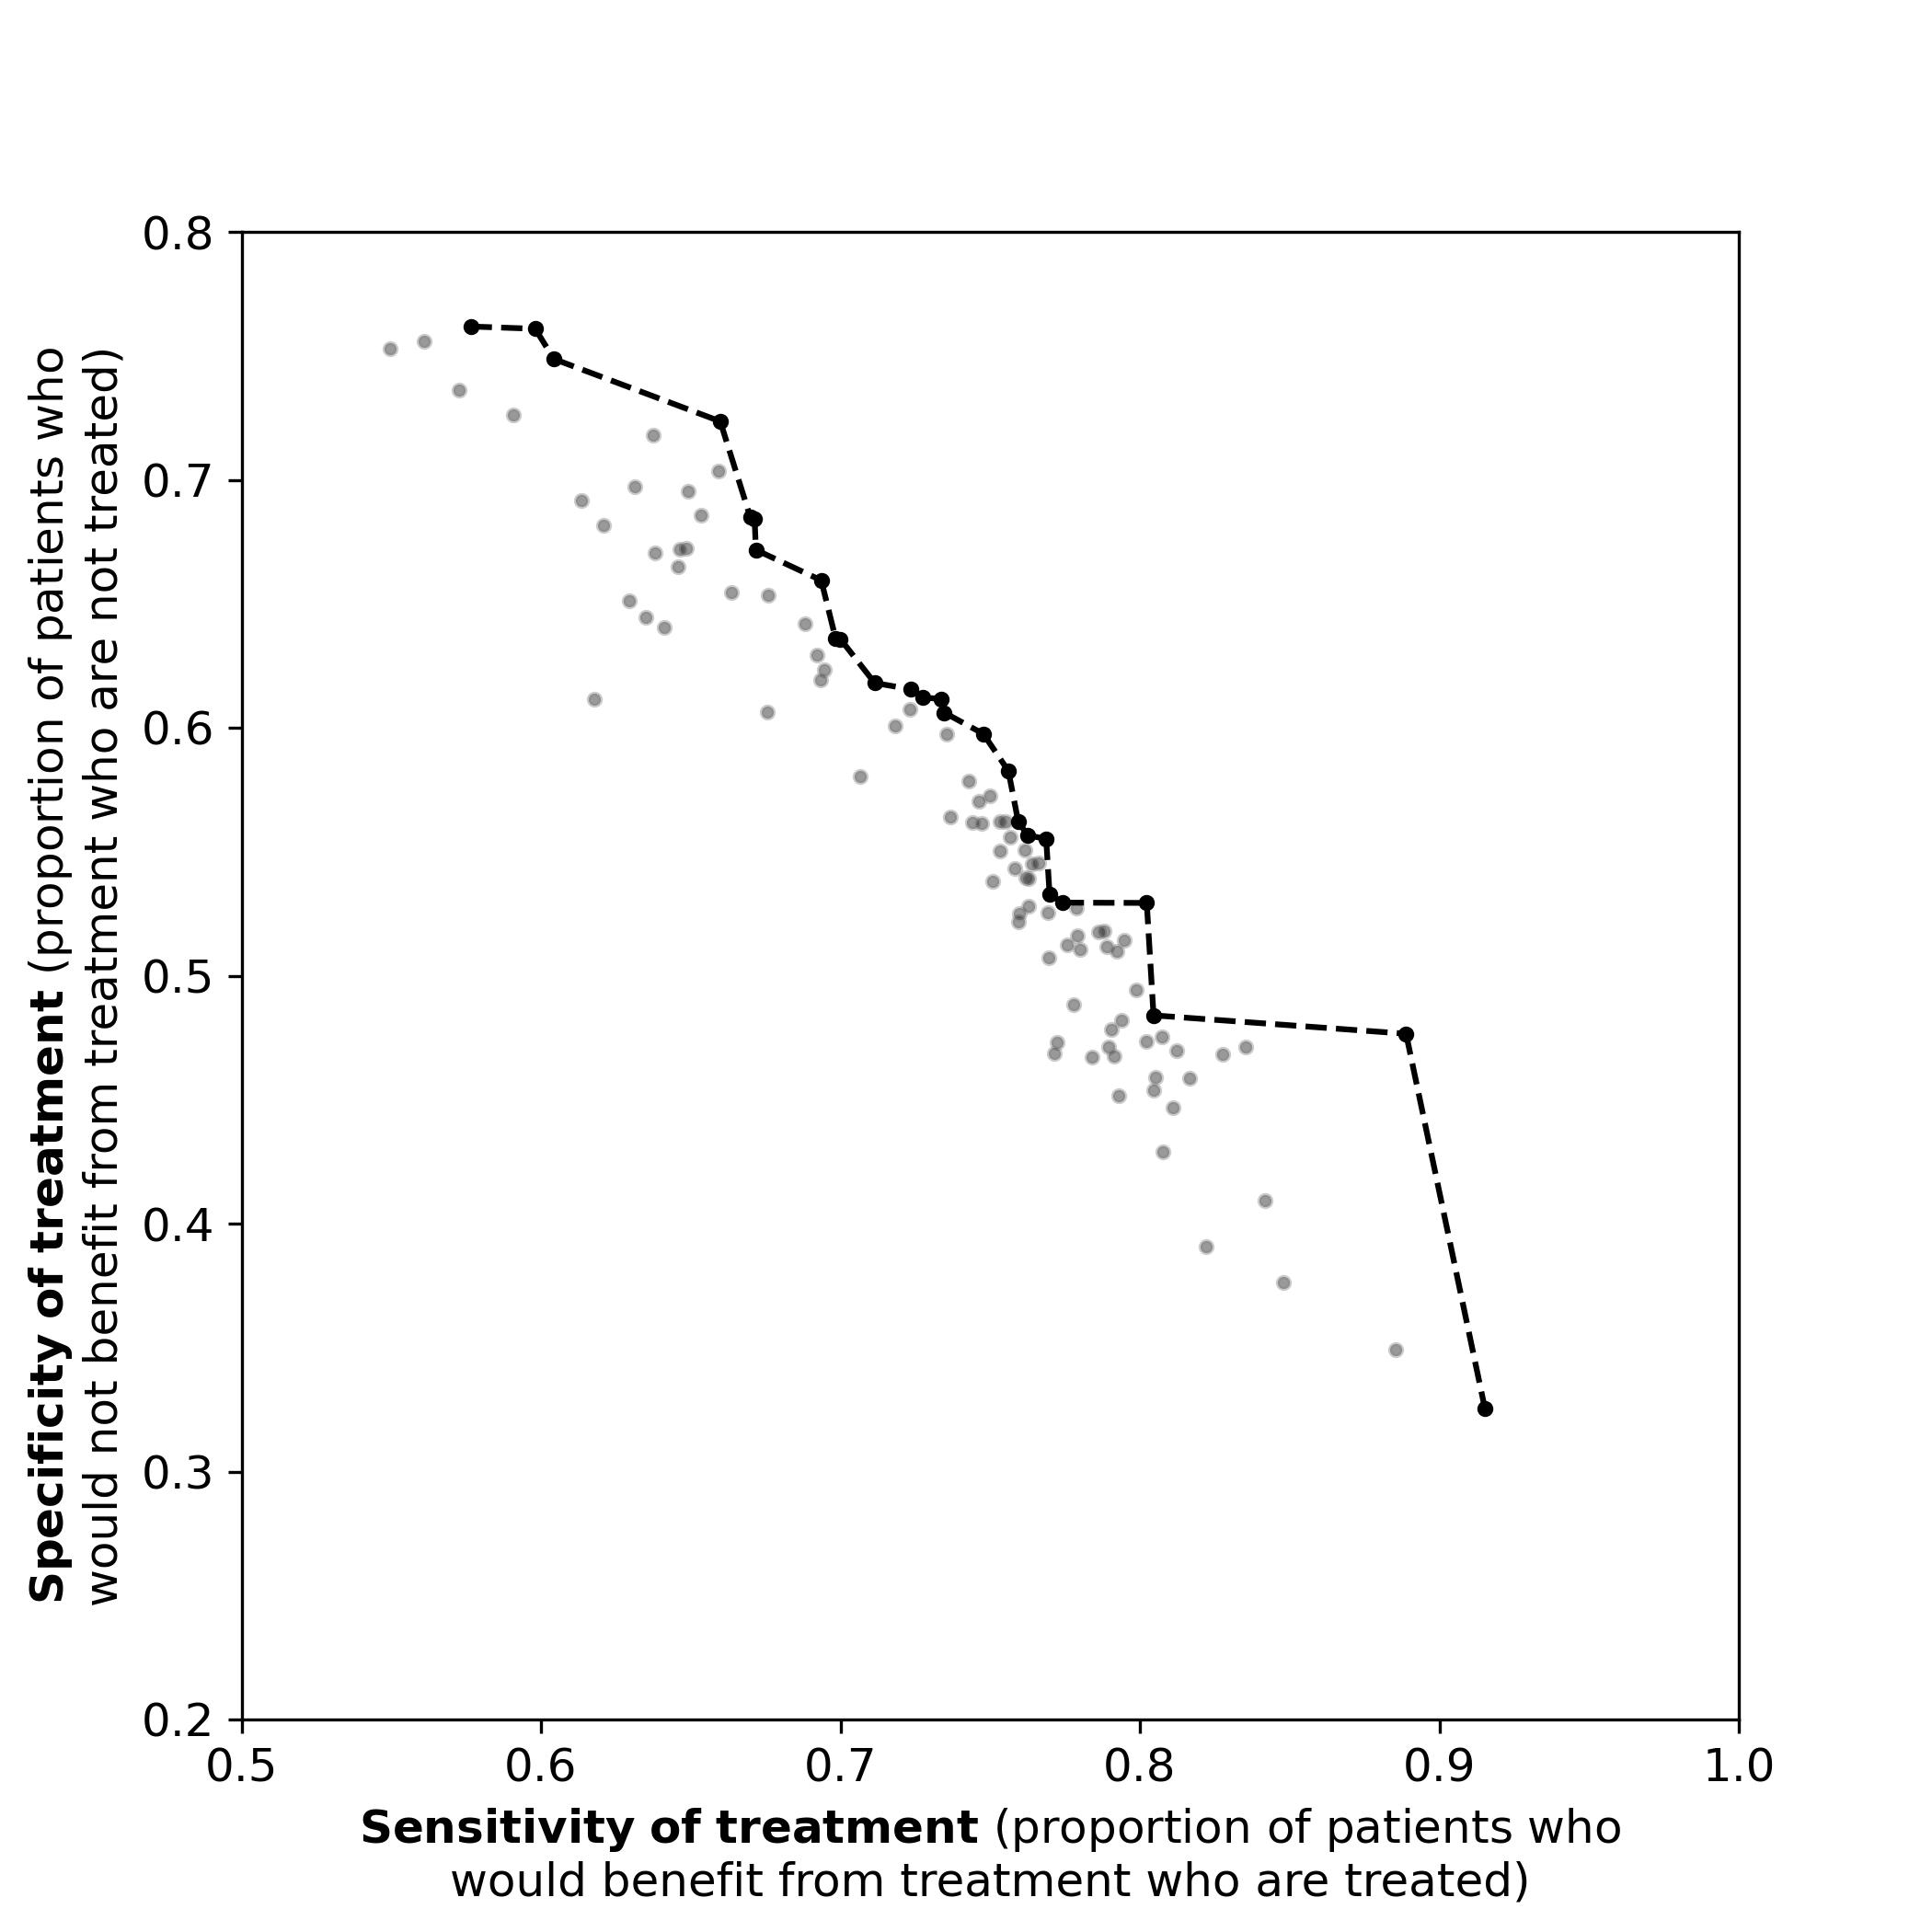
\includegraphics[width=3.5in]{./images/210_xgb_all_data_multiclass_outcome_spec_sens.jpg}}\\ 
    \caption{\textit{Sensitivity} (proportion of patients who were predicted to benefit from thrombolysis who were predicted to receive thrombolysis) and \textit{specificity} (proportion of patients who were predicted \textit{not} to benefit from thrombolysis who were predicted \textit{not} to receive thrombolysis) for each stroke team. The dotted line shows the hospitals on the Pareto front where there are no hospitals that have a better \textit{sensitivity} without a worse \textit{specificity}, or vice-versa.}
    \label{fig:hosp_shap_scatter}
\end{figure}
\section{Discussion}

%%%%%% INCLUDE %%%%%%

% Summarise main points
% Compare to other work
% Clinical significance
% Limitations & future work


%%%%%%%%%%%%% Summarise main points %%%%%%%%%%%%%
As thrombolysis carries a risk of harm (principally brain haemorrhage), determining whether a patient is likely to have an improved outcome with thrombolysis requires considering whether there is likely to be an average improvement in disability score (the mid point of predicted discharge disability probabilities), and whether there could be an increased risk of severe harm, which we defined as a disability at discharge of mRS 5-6 (severe disability or death). In order to create a simpler category of `improved outcome' with thrombolysis we took a conservative view that there should be better predicted average outcomes and a reduction of risk of death or severe disability. In this work we did not model risk of haemorrhage in isolation as we wished to focus on all-cause outcomes and overall net benefit/risk of thrombolysis.

We found general agreement between actual thrombolysis use and best predicted outcomes, though we found decisions based on the outcome model would support higher use of thrombolysis than is actually the case. Of those who did not receive thrombolysis, the outcome model predicted that nearly half of them would have likely benefited from thrombolysis. Of those that did receive thrombolysis we found about one in four may be being given thrombolysis without there being predicted benefit. Of those receiving thrombolysis when they would likely not benefit from it, or vice-versa, we found no simple way to identify patients from any individual patient feature; it is a combination of patient features that affect whether a patient will likely receive benefit from thrombolysis or not. For example, the chance of benefit is improved with more severe stroke or earlier use of thrombolysis. As such, with milder stroke, it may be necessary to give thrombolysis earlier (all other patient characteristics beings equal) in order to achieve net benefit. Such interaction effects on outcome are not easy to capture in binary cut-offs, such as those described by stroke severity or time limits commonly used in clinical guidelines.

We found that the hospital attended affected reported outcome after stroke, after allowing for other patient characteristics. This could be due to 1) some hospitals discharging earlier and with more disability (e.g. with community rehabilitation available), 2) effects of other hospital treatments on outcomes (e.g. better/worse stroke unit care), or 3) hospitals assessing disability at discharge differently. From our model we cannot speculate further, but by including stroke team in the model we adjust the model for these effects, allowing a clearer view of other patient features affecting outcome.

There was an apparent trade-off in decision-making between hospitals. Those hospitals who gave thrombolysis to more patients who would benefit from it (higher \textit{sensitivity}) were also more likely to give thrombolysis to more patients who would not benefit from it (lower \textit{specificity}). This represents a trade-off between `\textit{Miss no benefit}' and `\textit{Do no harm}'. Maximising benefit while minimising harm is likely to require more sophisticated guidance on use of thrombolysis, such as that indicated by our model.

In order to compare decisions and outcomes for key parts of the analysis we simplified the outcome in a dichotomised \textit{good} vs \textit{bad}. The spread of benefit and disbenefit showed many patients may be at the border of benefit and disbenefit which is obscured to some extent with the dichotomised outcome. We used a conservative measure of a good outcome where the average disability should be improved while also reducing the risk of the worst outcomes. Of those we classified as a bad outcome from thrombolysis, two thirds had an improvement in \textit{either} average disability or probability of being discharged mRS 5-6.  

%%%%%%%%%%%%% Compare to other work %%%%%%%%%%%%%

Our work supports that use of thrombolysis can improve outcome in many stroke patients (see our companion paper comparing our observed benefit of thrombolysis to clinical trials \cite{pearn_thrombolysis_2024}) and many patients may currently be missing benefit. In previous work we have identified that willingness to use thrombolysis differs between stroke teams \cite{allen_use_2022, allen_using_2022}. In this current work we observe that this willingness to use thrombolysis is associated with a predicted trade off between sensitivity (not missing benefit) and specificity (not doing harm) of treatment.

%%%%%%%%%%%%% Clinical significance %%%%%%%%%%%%%

The major significance of this work is that there appears to be potential to improve use of thrombolysis both by increasing use of thrombolysis (many patients appear to be missing the benefit of thrombolysis), but also by better targeting of thrombolysis to avoid those patients more likely to be harmed by thrombolysis. It is possible that, while not perfect, better use and targeting of thrombolysis could be achieved by some simple algorithm (such as a decision-tree that requires no on-scene computational prediction). 

%%%%%%%%%%%%% Limitations & future work %%%%%%%%%%%%%

\subsection{Study limitations and further work}

Our model is limited to data available in SSNAP. Though the accuracy overall is good, it is not intended for individual clinical decision-making. There may be unmeasured factors not in SSNAP that are contributing to the decision to treat and to outcomes. Our focus was on overall patterns present in the data. In the absence of individual patient-level predictions, we suggest future work should focus on providing more sophisticated guidance (though without requiring specialist models) on selection of patients for thrombolysis. There is also significant scope to use the same techniques to study variation in use of thrombectomy, and how that variation affects patient outcomes.

The outcome measure available for the study to use, mRS at discharge, is a measure of independence, and as such, may not capture other life changing symptoms of stroke, such as mental and cognitive healthy and well-being.

In the current study we predicted overall outcome, rather than specifically estimating risk of thrombolysis-induced haemorrhage. Future work could investigate separate risk and benefit models (separately predicting risk of thrombolysis-induced haemorrhage and benefit only in absence of thrombolysis-induced haemorrhage). 

%\include{sections/07_references}


\section{References}
\bibliographystyle{naturemag}
%\bibliographystyle{plainnat}
%\bibliographystyle{unsrt}
%\bibliographystyle{unsrtnat}
\bibliography{references}

\newpage
\section*{Acknowledgements}

We would like to thank the SAMueL project team (Lauren Asare, Julia Frost, Iain Lang, Kristin Liabo, Peter McMeekin, Keira Pratt-Boyden, Cathy Pope, Ken Stein, Penny Thompson, Rachel Jarvie) for their input into this work. We would also like to thank our Patient and Carer Involvement team led by Leon Farmer (David Burgess, Simon Douglas, Ian Hancock, Nicola Hancock, John Williams), and our expert advisory group (Ajay Bhalla, Gary Ford, Martin Utley).

\section*{Declaration of conflicting interests}

The authors declare no potential conflicts of interest with respect to the research, authorship, and/or publication of this article. 

\section*{Funding}

The authors disclose receipt of the following financial support for the research, authorship, and/or publication of this article: This research was funded by the National Institute for Health Research Applied Research Collaboration South West Peninsula and by the National Institute for Health Research Health and Social Care Delivery Research (HSDR) Programme [NIHR134326]. The views expressed in this publication are those of the authors and not necessarily those of the National Institute for Health Research or the Department of Health and Social Care. 

\section*{Informed consent and Ethics}

As we are using anonymised secondary data, collected for national audit, individual consent is not required. SSNAP has approval under section 251 of the NHS Health and Social Care Act (2006) to collect patient level data on the first six months of patient care (ECC 6- 02(FT3)/2012), without requiring individual patient consent. Access to SSNAP data is managed by the UK Healthcare Quality Improvement Partnership (HQIP), with this project being approved by HQIP (HQIP303). More information on SSNAPs use of patient data may be found at: https://www.strokeaudit.org/ SupportFiles/Documents/Patient-area-documents/Fair-processingstatement-for-patients-v7-0.aspx

As we are using anonymised secondary data, collected for national audit, used for service evaluation and improvement, no ethical approval is required (confirmed using the NHS Health Research Authority decision aid: https://www.hra-decisiontools.org.uk/ethics/).

\section*{Guarantor}

The corresponding author, Michael Allen, is the guarantor of the paper (PI on the NIHR project funding).

% Number for supplementary material
\newcommand{\beginsupplement}{
    \setcounter{section}{0}
    \renewcommand{\thesection}{S\arabic{section}}
    \setcounter{figure}{0}
    \renewcommand{\thefigure}{S\arabic{figure}}
    \setcounter{table}{0}
    \renewcommand{\thetable}{S\arabic{table}}
}

\beginsupplement
%\section{Supplementary material}

\subsection{Descriptive statistics}

General descriptive statistics of patients in the retrieved SSNAP data set is shown in tables \ref{tab:hospital_stats_1} and \ref{tab:hospital_stats_2}.

\small
\renewcommand{\arraystretch}{1.3}
\begin{longtable}{p{7cm} p{1cm} p{0.8cm} p{0.8cm} p{0.8cm} p{0.8cm} p{0.8cm} p{0.8cm} p{0.8cm} p{0.8cm}}
\caption{Descriptive statistics for all patients arriving at each stroke team. The table shows summary statistics across all stroke teams.}\\
\toprule
\endhead
Statistic & Stroke teams & mean & Std Dev & min & 25\% & 50\% & 75\% & max\tabularnewline
\midrule
Yearly admissions & 119 & 509 & 208 & 95 & 372 & 489 & 627 & 1183\tabularnewline
Age (mean) & 119 & 74 & 2 & 65 & 73 & 75 & 76 & 78\tabularnewline
Proportion aged 80+ & 119 & 0.40 & 0.06 & 0.20 & 0.36 & 0.40 & 0.44 & 0.51\tabularnewline
Proportion male & 119 & 0.53 & 0.02 & 0.47 & 0.51 & 0.53 & 0.55 & 0.60\tabularnewline
Prior disability (mRS, mean) & 119 & 1.02 & 0.25 & 0.29 & 0.87 & 1.03 & 1.21 & 1.60\tabularnewline
Proportion prior disability (mRS) 0-2 & 119 & 0.81 & 0.05 & 0.67 & 0.78 & 0.81 & 0.84 & 0.97\tabularnewline
Proportion ischaemic stroke & 119 & 0.88 & 0.02 & 0.83 & 0.86 & 0.88 & 0.89 & 0.93\tabularnewline
Stroke severity (NIHSS, mean) & 119 & 7.0 & 1.0 & 4.6 & 6.3 & 7.2 & 7.8 & 9.1\tabularnewline
Proportion with known onset & 119 & 0.68 & 0.14 & 0.43 & 0.58 & 0.67 & 0.76 & 1.00\tabularnewline
Onset-to-arrival time (minutes, median) & 119 & 204 & 76 & 109 & 155 & 180 & 224 & 466\tabularnewline
Proportion arriving within 4 hours known onset & 119 & 0.38 & 0.06 & 0.19 & 0.34 & 0.38 & 0.43 & 0.51\tabularnewline
Proportion with precisely known onset & 119 & 0.33 & 0.11 & 0.01 & 0.28 & 0.34 & 0.39 & 0.63\tabularnewline
Proportion onset during sleep & 119 & 0.14 & 0.06 & 0.00 & 0.09 & 0.14 & 0.17 & 0.34\tabularnewline
Proportion arrive by ambulance & 119 & 0.78 & 0.07 & 0.47 & 0.76 & 0.79 & 0.82 & 0.92\tabularnewline
Call-to-ambulance arrival time (minutes, median) & 113 & 22 & 10 & 13 & 17 & 20 & 24 & 103\tabularnewline
Ambulance on scene time (median) & 113 & 31 & 3 & 20 & 28 & 31 & 33 & 41\tabularnewline
Ambulance conveyance time (minutes, median) & 113 & 18 & 5 & 10 & 15 & 17 & 21 & 37\tabularnewline
Arrival-to-scan time (minutes, median) & 119 & 53 & 21 & 13 & 39 & 51 & 63 & 129\tabularnewline
Proportion receiving thrombolysis & 119 & 0.115 & 0.034 & 0.021 & 0.092 & 0.110 & 0.136 & 0.245\tabularnewline
Scan-to-thrombolysis time (minutes, median) & 119 & 34 & 10 & 14 & 28 & 34 & 41 & 72\tabularnewline
Discharge disability (mRS, mean) & 119 & 2.641 & 0.352 & 1.361 & 2.413 & 2.699 & 2.900 & 3.320\tabularnewline
Proportion discharged mRS 0-2 & 119 & 0.524 & 0.095 & 0.293 & 0.454 & 0.522 & 0.594 & 0.799\tabularnewline
Proportion discharged mRS 5-6 & 119 & 0.195 & 0.037 & 0.095 & 0.170 & 0.198 & 0.218 & 0.287\tabularnewline
\bottomrule
\label{tab:hospital_stats_1}
\end{longtable}
\normalsize

\small
\begin{longtable}{p{7cm} p{1cm} p{0.8cm} p{0.8cm} p{0.8cm} p{0.8cm} p{0.8cm} p{0.8cm} p{0.8cm} p{0.8cm}}
\caption{Descriptive statistics for patients arriving at each stroke team, for patients arriving within 4 hours of known stroke onset. The table shows summary statistics across all stroke teams.}\\
\toprule
\endhead
Statistic & Stroke teams & mean & Std Dev & min & 25\% & 50\% & 75\% & max\tabularnewline
\midrule
Yearly admissions & 119 & 193 & 78 & 28 & 139 & 183 & 241 & 428\tabularnewline
Age (mean) & 119 & 75 & 2 & 66 & 73 & 75 & 76 & 79\tabularnewline
Proportion aged 80+ & 119 & 0.41 & 0.06 & 0.23 & 0.37 & 0.41 & 0.45 & 0.57\tabularnewline
Proportion male & 119 & 0.53 & 0.03 & 0.45 & 0.51 & 0.53 & 0.55 & 0.64\tabularnewline
Prior disability (mRS, mean) & 119 & 1.04 & 0.25 & 0.37 & 0.88 & 1.04 & 1.22 & 1.60\tabularnewline
Proportion prior disability (mRS) 0-2 & 119 & 0.80 & 0.06 & 0.66 & 0.77 & 0.81 & 0.83 & 0.95\tabularnewline
Proportion ischaemic stroke & 119 & 0.85 & 0.03 & 0.75 & 0.84 & 0.85 & 0.87 & 0.94\tabularnewline
Stroke severity (NIHSS, mean) & 119 & 8.9 & 1.1 & 6.4 & 8.2 & 9.0 & 9.7 & 11.4\tabularnewline
Proportion with known onset & 119 & 1.00 & 0.00 & 1.00 & 1.00 & 1.00 & 1.00 & 1.00\tabularnewline
Onset-to-arrival time (minutes, median) & 119 & 105 & 9 & 85 & 100 & 105 & 111 & 132\tabularnewline
Proportion arriving within 4 hours known onset & 119 & 1.00 & 0.00 & 1.00 & 1.00 & 1.00 & 1.00 & 1.00\tabularnewline
Proportion with precisely known onset & 119 & 0.62 & 0.17 & 0.02 & 0.54 & 0.66 & 0.75 & 0.91\tabularnewline
Proportion onset during sleep & 119 & 0.05 & 0.05 & 0.00 & 0.01 & 0.03 & 0.06 & 0.30\tabularnewline
Proportion arrive by ambulance & 119 & 0.89 & 0.07 & 0.54 & 0.87 & 0.91 & 0.93 & 0.98\tabularnewline
Call-to-ambulance arrival time (minutes, median) & 110 & 19 & 5 & 8 & 16 & 18 & 21 & 51\tabularnewline
Ambulance on scene time (median) & 110 & 28 & 4 & 20 & 26 & 28 & 31 & 46\tabularnewline
Ambulance conveyance time (minutes, median) & 110 & 17 & 4 & 9 & 14 & 16 & 20 & 28\tabularnewline
Arrival-to-scan time (minutes, median) & 119 & 27 & 11 & 4 & 21 & 28 & 34 & 100\tabularnewline
Proportion receiving thrombolysis & 119 & 0.293 & 0.070 & 0.111 & 0.250 & 0.282 & 0.333 & 0.534\tabularnewline
Scan-to-thrombolysis time (minutes, median) & 119 & 34 & 10 & 14 & 28 & 34 & 40 & 71\tabularnewline
Discharge disability (mRS, mean) & 119 & 2.803 & 0.353 & 1.507 & 2.609 & 2.837 & 3.039 & 3.663\tabularnewline
Proportion discharged mRS 0-2 & 119 & 0.494 & 0.094 & 0.209 & 0.424 & 0.495 & 0.554 & 0.771\tabularnewline
Proportion discharged mRS 5-6 & 119 & 0.236 & 0.045 & 0.138 & 0.208 & 0.231 & 0.256 & 0.420\tabularnewline
\bottomrule
\label{tab:hospital_stats_2}
\end{longtable}
\normalsize

\small
\begin{longtable}{p{7cm} p{1cm} p{0.8cm} p{0.8cm} p{0.8cm} p{0.8cm} p{0.8cm} p{0.8cm} p{0.8cm} p{0.8cm}}
\caption{Descriptive statistics for patients arriving at each stroke team, for patients arriving by ambulance within 4 hours of known stroke onset. The table shows summary statistics across all stroke teams.}\\
\toprule
\endhead
Statistic & Stroke teams & mean & Std Dev & min & 25\% & 50\% & 75\% & max\tabularnewline
\midrule
Yearly admissions & 119 & 173 & 74 & 15 & 125 & 163 & 227 & 400\tabularnewline
Age (mean) & 119 & 75 & 2 & 66 & 74 & 76 & 77 & 81\tabularnewline
Proportion aged 80+ & 119 & 0.43 & 0.06 & 0.24 & 0.39 & 0.43 & 0.47 & 0.62\tabularnewline
Proportion male & 119 & 0.52 & 0.03 & 0.45 & 0.51 & 0.52 & 0.54 & 0.60\tabularnewline
Prior disability (mRS, mean) & 119 & 1.10 & 0.25 & 0.46 & 0.94 & 1.09 & 1.26 & 1.66\tabularnewline
Proportion prior disability (mRS) 0-2 & 119 & 0.79 & 0.06 & 0.65 & 0.75 & 0.79 & 0.83 & 0.93\tabularnewline
Proportion ischaemic stroke & 119 & 0.85 & 0.03 & 0.75 & 0.83 & 0.85 & 0.87 & 0.94\tabularnewline
Stroke severity (NIHSS, mean) & 119 & 9.4 & 1.2 & 6.7 & 8.6 & 9.5 & 10.2 & 12.2\tabularnewline
Proportion with known onset & 119 & 1.00 & 0.00 & 1.00 & 1.00 & 1.00 & 1.00 & 1.00\tabularnewline
Onset-to-arrival time (minutes, median) & 119 & 106 & 10 & 84 & 99 & 105 & 112 & 151\tabularnewline
Proportion arriving within 4 hours known onset & 119 & 1.00 & 0.00 & 1.00 & 1.00 & 1.00 & 1.00 & 1.00\tabularnewline
Proportion with precisely known onset & 119 & 0.62 & 0.17 & 0.02 & 0.54 & 0.65 & 0.75 & 0.92\tabularnewline
Proportion onset during sleep & 119 & 0.05 & 0.05 & 0.00 & 0.01 & 0.03 & 0.06 & 0.33\tabularnewline
Proportion arrive by ambulance & 119 & 1.00 & 0.00 & 1.00 & 1.00 & 1.00 & 1.00 & 1.00\tabularnewline
Call-to-ambulance arrival time (minutes, median) & 110 & 19 & 5 & 8 & 16 & 18 & 21 & 51\tabularnewline
Ambulance on scene time (median) & 110 & 28 & 4 & 20 & 26 & 28 & 31 & 46\tabularnewline
Ambulance conveyance time (minutes, median) & 110 & 17 & 4 & 9 & 14 & 16 & 20 & 28\tabularnewline
Arrival-to-scan time (minutes, median) & 119 & 26 & 11 & 4 & 20 & 25 & 33 & 95\tabularnewline
Proportion receiving thrombolysis & 119 & 0.300 & 0.072 & 0.130 & 0.252 & 0.289 & 0.345 & 0.537\tabularnewline
Scan-to-thrombolysis time (minutes, median) & 119 & 34 & 10 & 13 & 27 & 33 & 40 & 73\tabularnewline
Discharge disability (mRS, mean) & 119 & 2.926 & 0.352 & 1.867 & 2.717 & 2.928 & 3.150 & 3.819\tabularnewline
Proportion discharged mRS 0-2 & 119 & 0.465 & 0.096 & 0.184 & 0.398 & 0.462 & 0.524 & 0.696\tabularnewline
Proportion discharged mRS 5-6 & 119 & 0.254 & 0.051 & 0.147 & 0.221 & 0.253 & 0.280 & 0.486\tabularnewline
\bottomrule
\label{tab:hospital_stats_3}
\end{longtable}
\normalsize


\subsection{Data}

Dataset includes the patient cohort (78,396) to make a clinical decision about whether to give thrombolysis:
\begin{enumerate}
    \item Ischaemic patients
    \item Have either/neither/both thrombolysis/thrombectomy.
    \item Not on anticoagulants.
    \item Arrive at hospital by ambulance after stroke onset.
    \item Have scan within 255 mins of stroke onset.
\end{enumerate}

\textbf{Summary of patient numbers during patient cohort creation}.
\begin{enumerate}
    \item Patients extracted (ischaemic, any/neither acute treatment, arrive at hospital by ambulance after stroke onset, have scan within 255 mins of stroke onset): 91,464
    \item Removed the 11,780 (12.9\%) patients on atrial fibrilation anticoagulants: 79,684
    \item Removed the 1,288 patients that attended hospitals with too few stroke admissions, or thrombolysis procedures: 78,396
\end{enumerate}
Of the 78,396 patient, 2,747 patients received thrombectomy, 75,649 did not.
Of the 75,649 patients not receive thrombectomy, 43,152 received thrombolysis and 32,497 did not.

The 78,396 patients attended 111 hospitals with admissions ranging from 267 to 1,414 (figure \ref{fig:admission_rate}), and thrombolysis rate ranging from 24\% to 67\%  (figure \ref{fig:thrombolysis_rate}). Of those 43,152 patients that do not receive thrombolysis (and not thrombectomy), 14\% has mRS0, 21\% have mRS1, 17\% have mRS2, 15\% have mRS3, 12\% have mRS4, 7\% have mRS5, and 13\% have mRS6 at discharge (figure \ref{fig:mrs_dist_wrt_ivt_bar}). Of those 32,497 patients that receive thrombolysis (and not thrombectomy), 15\% has mRS0, 21\% have mRS1, 18\% have mRS2, 16\% have mRS3, 12\% have mRS4, 5\% have mRS5, and 13\% have mRS6 at discharge (figure \ref{fig:mrs_dist_wrt_ivt_bar}).


\begin{figure}
    \centering
    \begin{subfigure}{.5\textwidth}
      \centering
      \captionsetup{width=.9\linewidth}
        {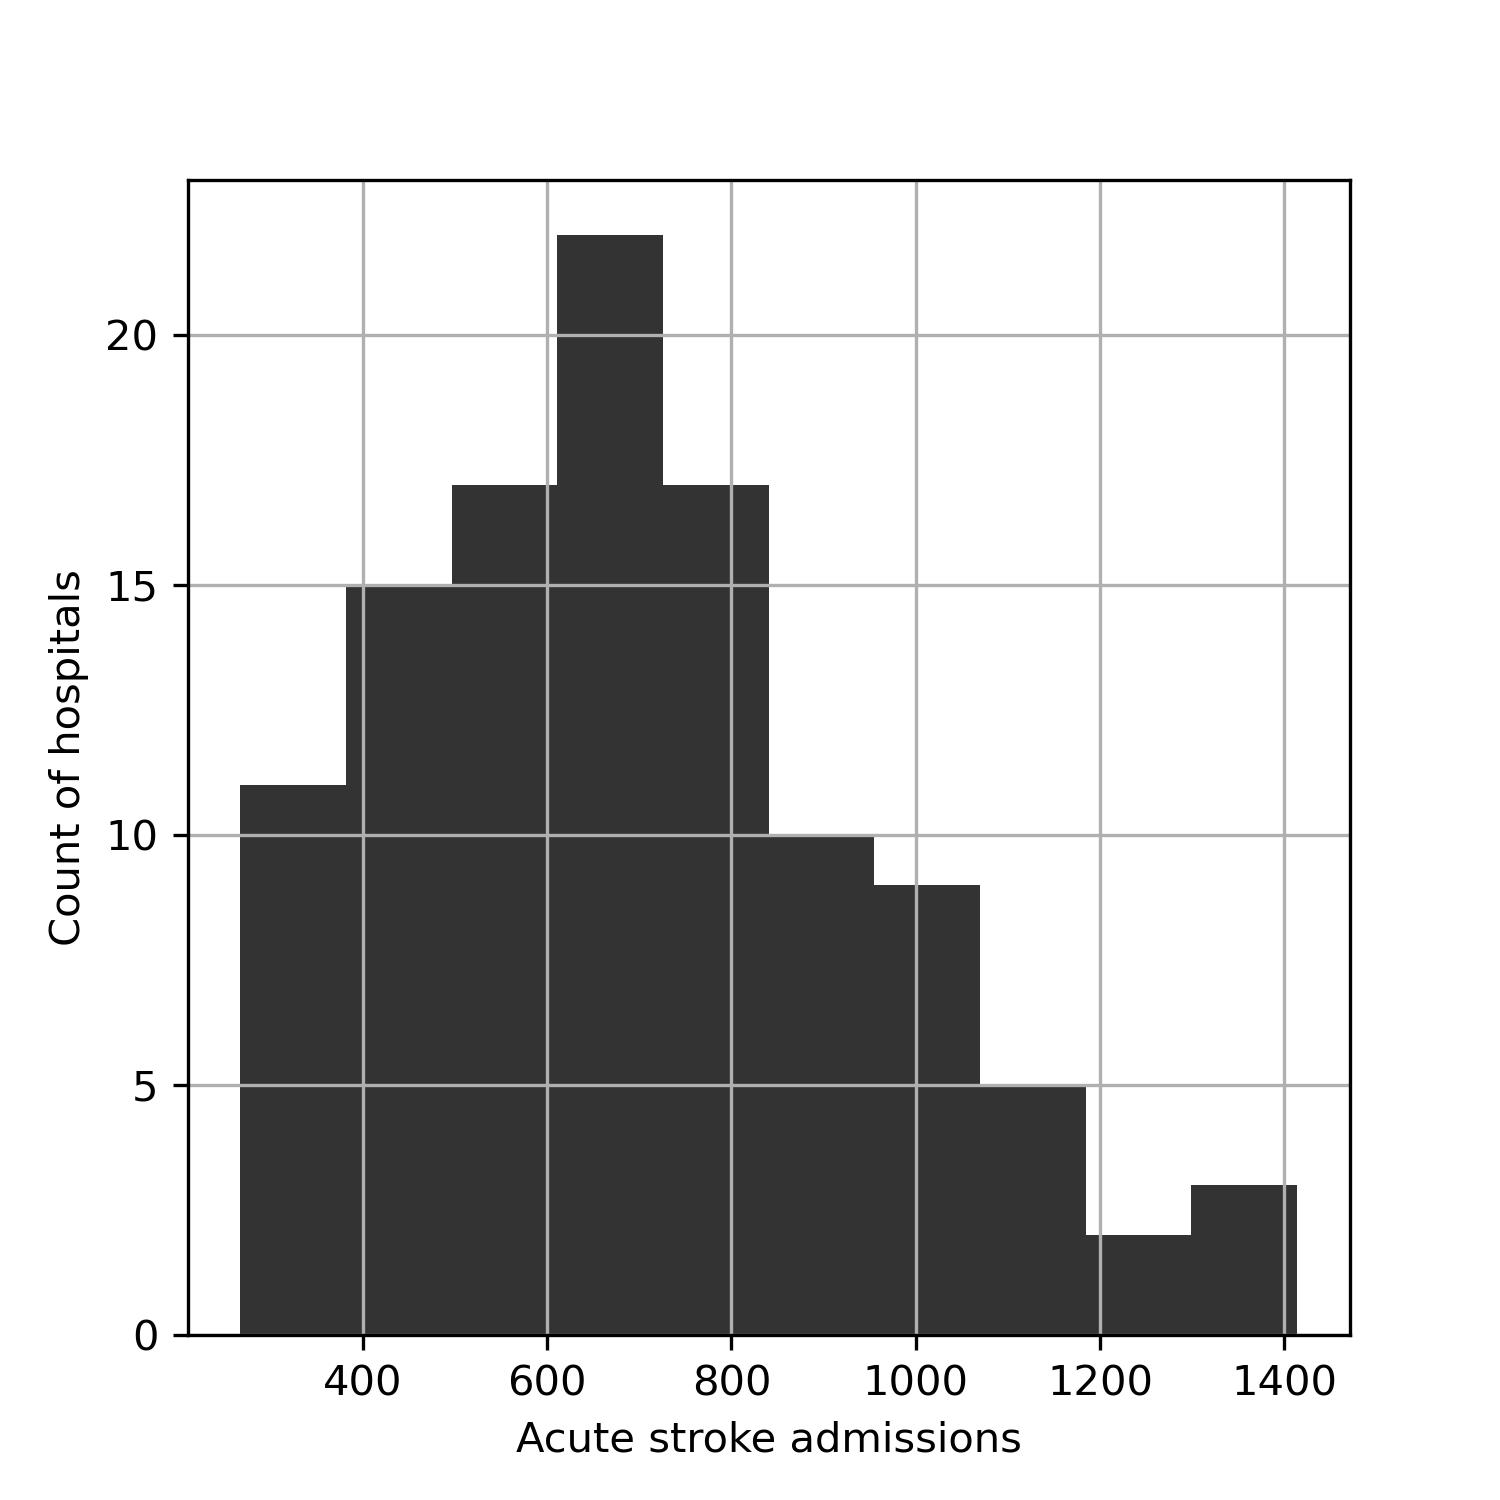
\includegraphics[width=0.95\linewidth]{./images/000_ssnap_descriptive_stats_admissions_hist}}\\
        \caption{Admissions to each of the 111 hospitals.}
        \label{fig:admission_rate}
        \end{subfigure}%ults
    \begin{subfigure}{.5\textwidth}
      \centering
      \captionsetup{width=.9\linewidth}
        {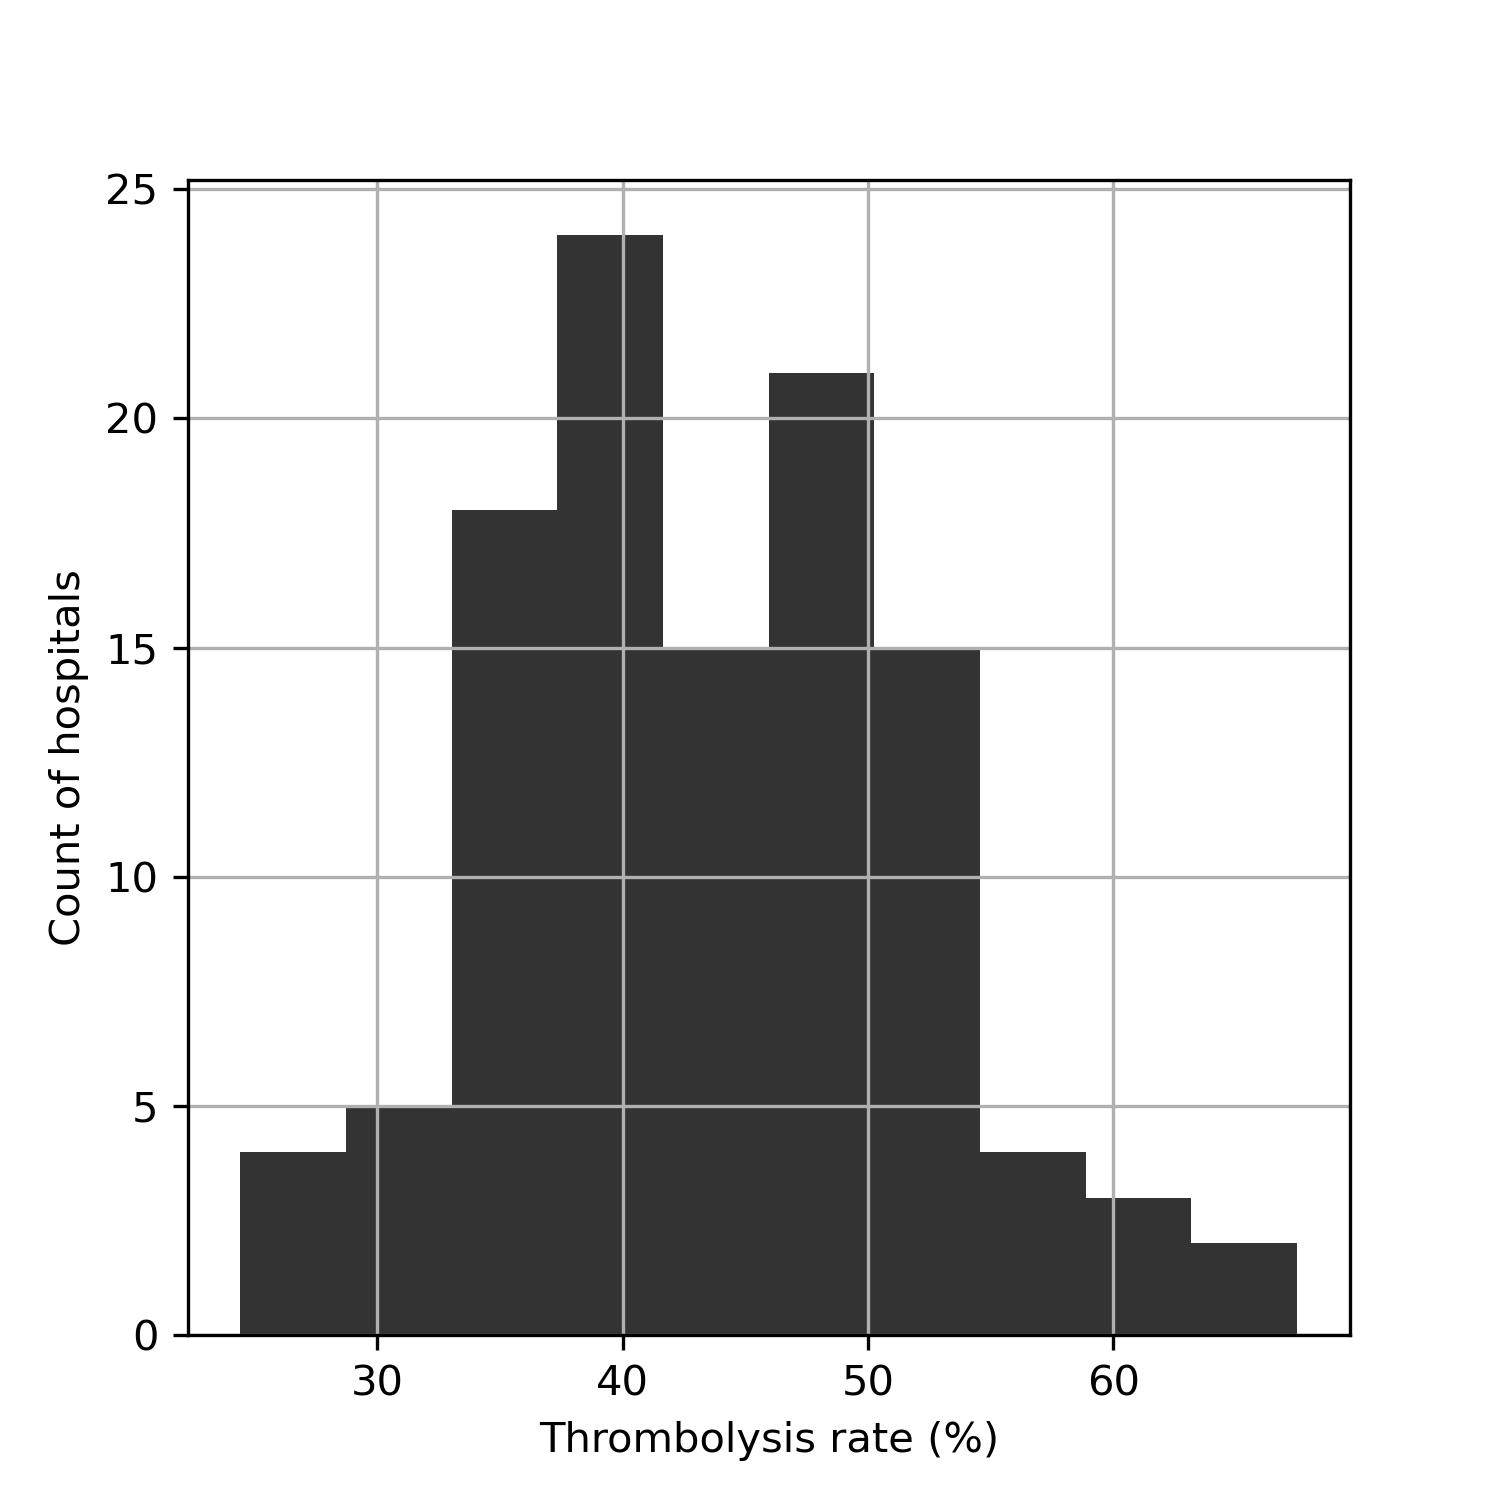
\includegraphics[width=0.95\linewidth]{./images/000_ssnap_descriptive_stats_thrombolysis_rate_hist}}\\
        \caption{Thrombolysis rate at each of the 111 hospitals}
        \label{fig:thrombolysis_rate}
    \end{subfigure}
    \caption{Histograms describing the hospitals}
\end{figure}

Figure \ref{fig:mrs_dist_wrt_ivt_bar} shows the distribution of mRS at discharge for two patient cohorts: those that receive thrombolysis, and those that do not.

\begin{figure}[h!]
    \centering
    {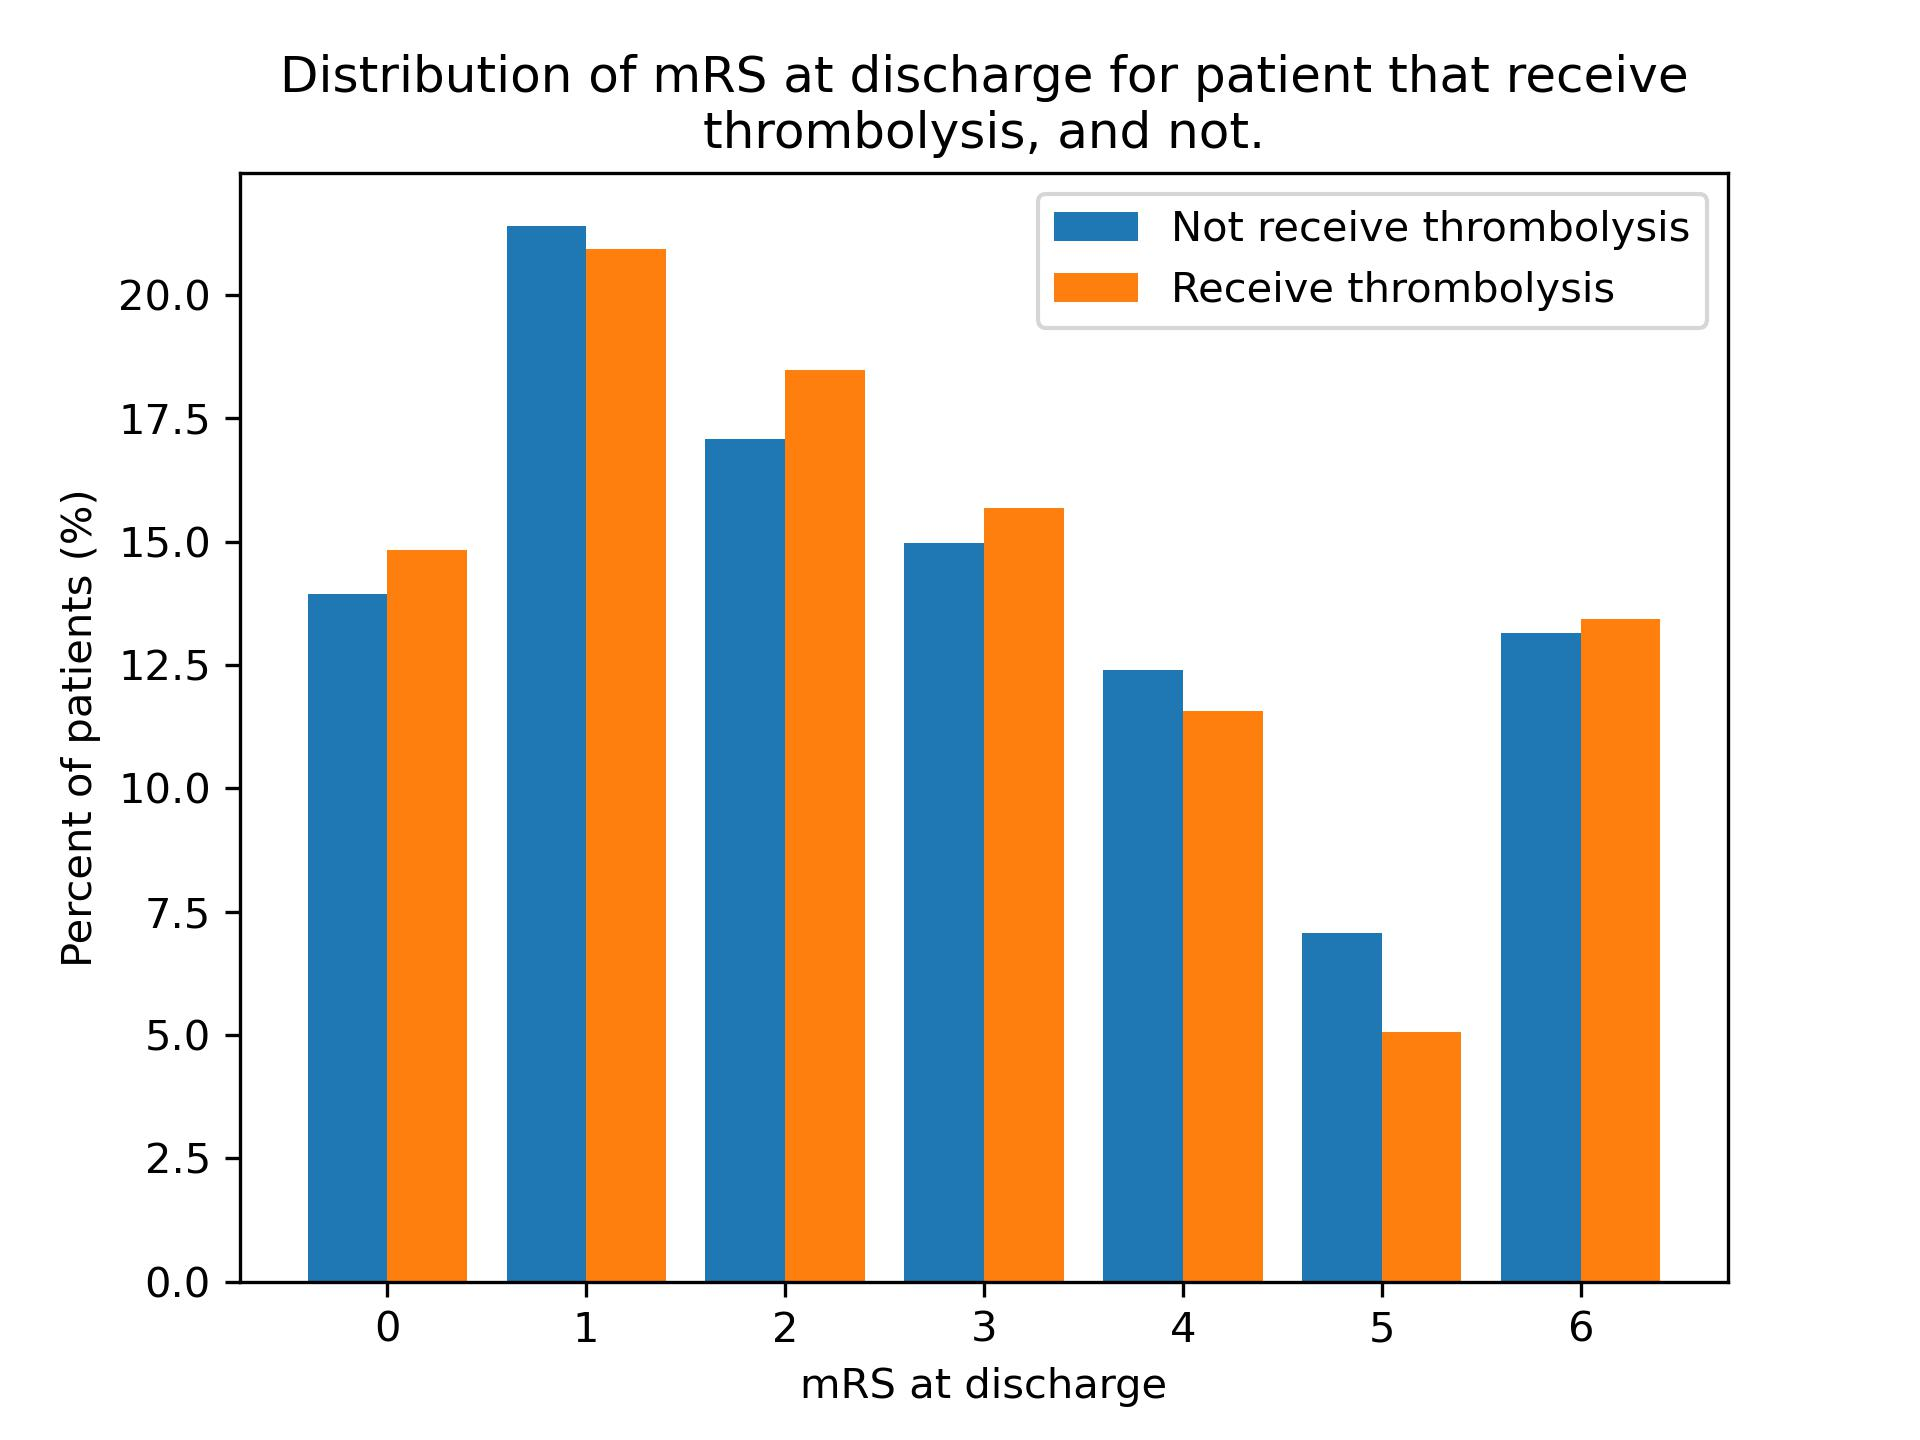
\includegraphics[width = 4in]{./images/000_ssnap_descriptive_stats_mrs_distribution_wrt_ivt.jpg}}\\
    \caption{Distribution of mRS at discharge, with respect to whether receive thrombolysis, or not.}
    \label{fig:mrs_dist_wrt_ivt_bar}
\end{figure}

\subsection{Learning curve}

We trained an XGBoost multiclass classification model to predict disability at discharge using all features as input, with a fixed 25\% test set, increment the training set size to assess whether we have enough data. Results are shown in fogure \ref{fig:learning_curve}.

\begin{figure}[h!]
    \centering
    {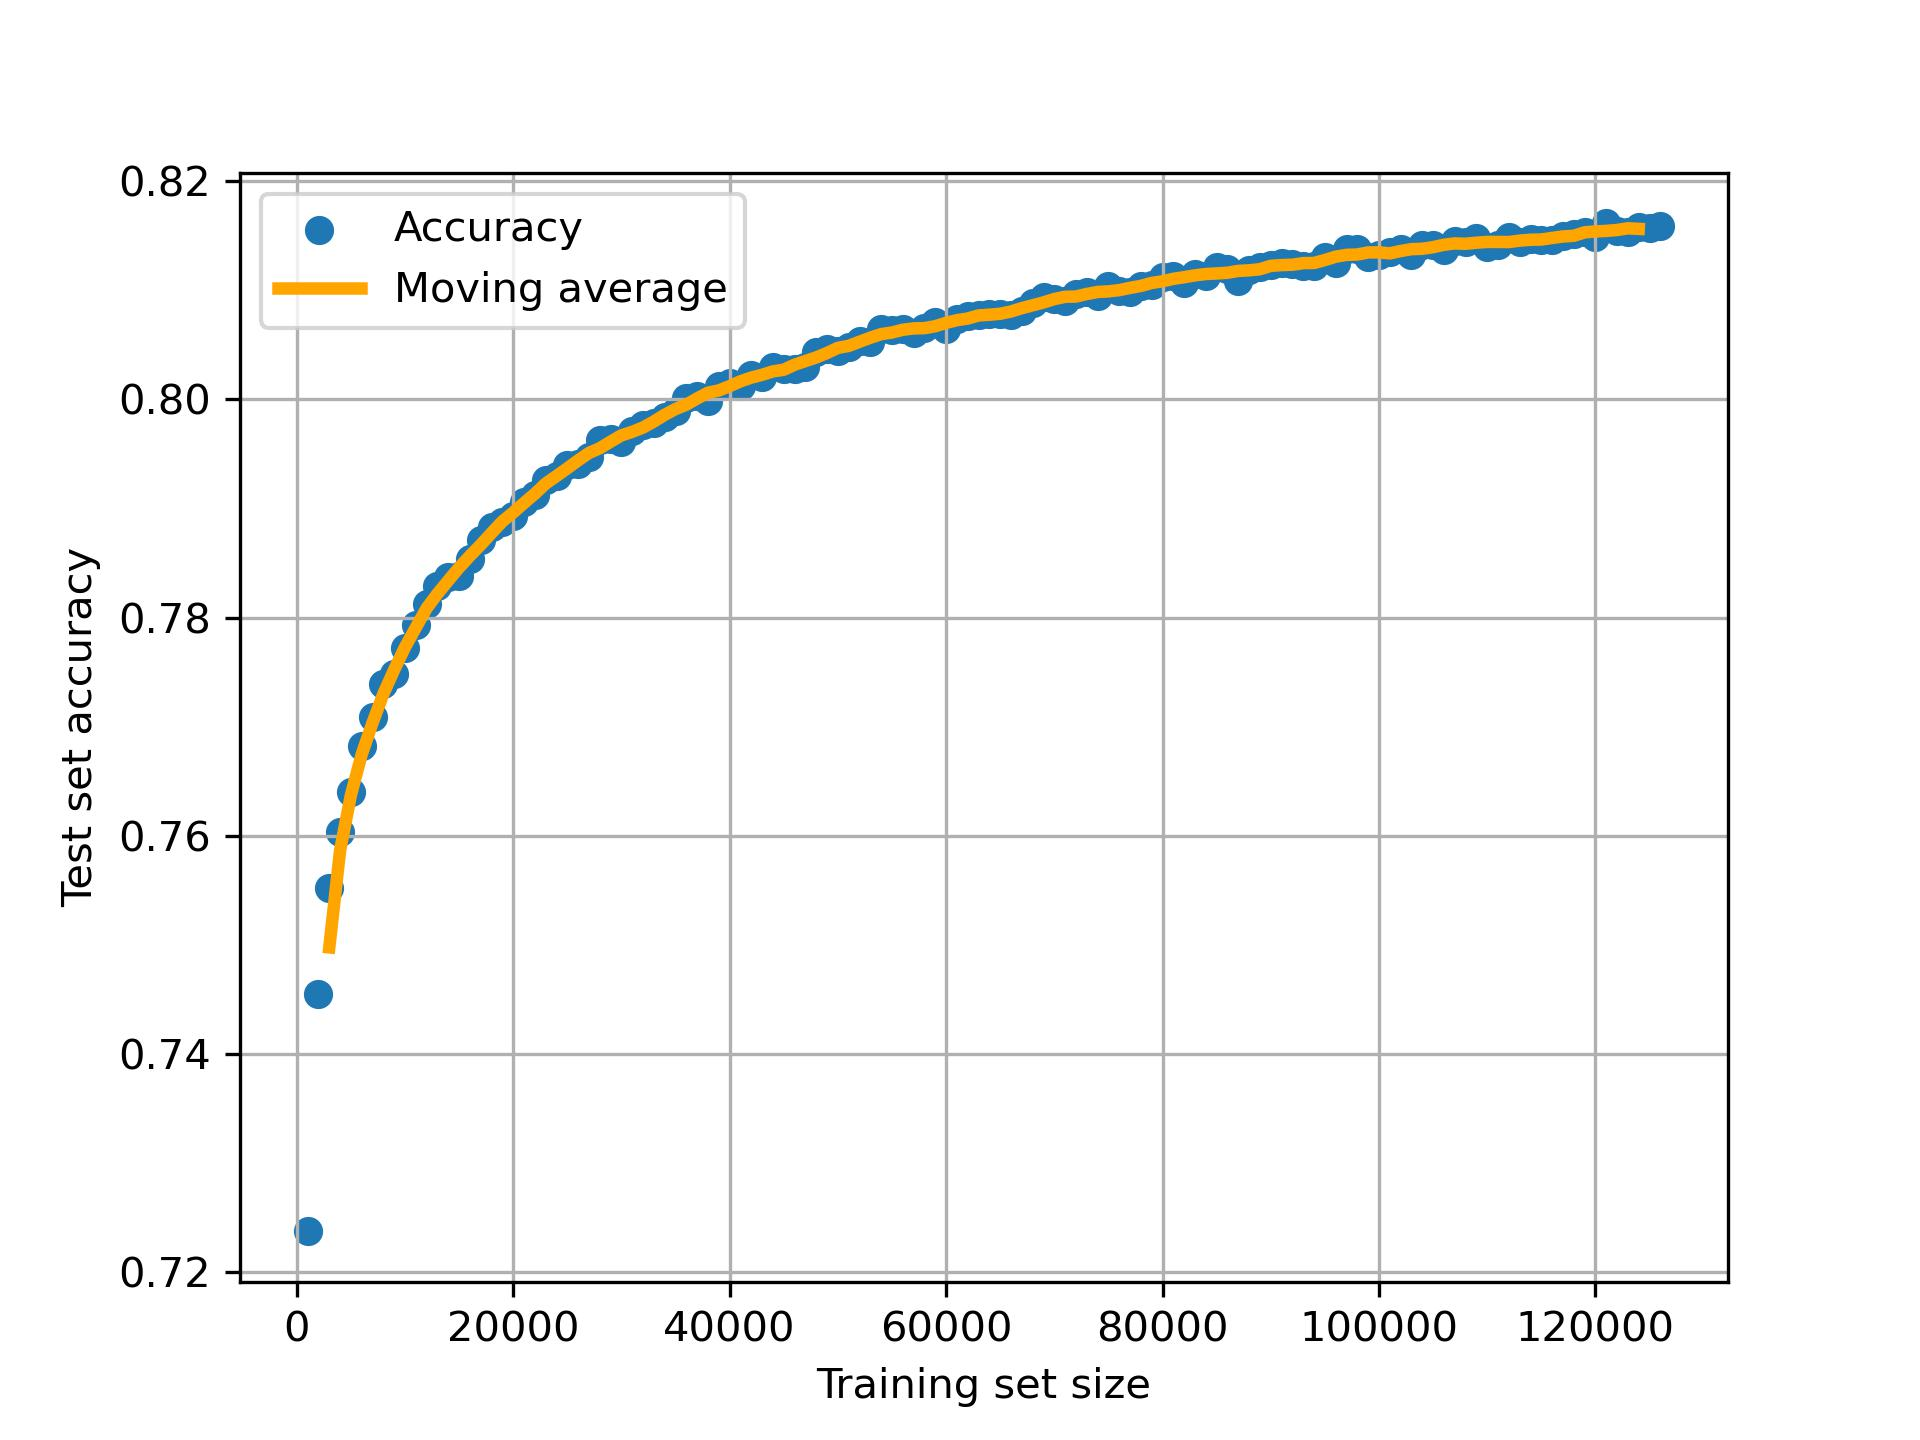
\includegraphics[width = 4in]{./images/015_xgb_all_features_learning_curve_learning_curve.jpg}}\\
    \caption{Learning rate. All features as input to the XGBoost thrombolysis outcome model (multiclass classification). Accuracy is measured as ROC-AUC.}
    \label{fig:learning_curve}
\end{figure}

\subsection{Feature selection}

Selecting which features (that describe the patients characteristics, their acute stroke pathway timings, use/time to thrombolysis, and the attended hospital) to include in an XGBoost multiclass classification model to predict disability at discharge.

\subsubsection{Model performance: All features}

The model performance with all 58 features is:
\begin{enumerate}
    \item AUC: 0.818 (std across 5 kfolds: 0.001)
    \item Accuracy: 0.440 (std across 5 kfolds: 0.002)
    \item Accuracy within one: 0.760 (std across 5 kfolds: 0.002)
\end{enumerate}

\subsubsection{Model performance: Sequentially selecting features}

Performance of models by sequentially adding the feature that incremented the performance (up to 25 features):
\begin{enumerate}
    \item prior\_disability, AUC: 0.687
    \item stroke\_severity, AUC: 0.770
    \item stroke\_team, AUC: 0.800
    \item age, AUC: 0.806
    \item year, AUC: 0.811
    \item nihss\_arrival\_loc, AUC: 0.814
    \item scan\_to\_thrombolysis\_time, AUC: 0.816
    \item thrombolysis\_no\_but\_improving, AUC: 0.817
    \item nihss\_arrival\_best\_language, AUC: 0.818
    \item new\_afib\_diagnosis, AUC: 0.818
    \item nihss\_arrival\_sensory, AUC: 0.819
    \item atrial\_fibrillation, AUC: 0.819
    \item nihss\_arrival\_facial\_palsy, AUC: 0.819
    \item thrombolysis\_no\_but\_other\_medical, AUC: 0.819
    \item infarction, AUC: 0.819
    \item arrive\_by\_ambulance, AUC: 0.819
    \item nihss\_arrival\_motor\_arm\_left, AUC: 0.819
    \item thrombolysis\_no\_but\_comorbidity, AUC: 0.819
    \item nihss\_arrival\_loc\_questions, AUC: 0.819
    \item nihss\_arrival\_motor\_arm\_right, AUC: 0.819
    \item nihss\_arrival\_best\_gaze, AUC: 0.820
    \item thrombolysis\_no\_but\_too\_mild\_severe, AUC: 0.820
    \item diabetes, AUC: 0.820
    \item thrombolysis\_no\_but\_haemorrhagic, AUC: 0.820
    \item thrombolysis\_no\_but\_medication, AUC: 0.820
\end{enumerate}

 With 15 features selected, the model choose a feature (infarction) that is the same value for all patients. We interpreted that to mean that no more information was being obtained beyond this point by adding a single feature.
 
\subsection{Feature selection - additional experiments}

To inform us further about which features to include in our model, we carried out some additional experiments. 

Here is what we learnt, and our selection of 7 features based on this:
\begin{enumerate}
    \item prior\_disability (easy selection choice)
    \item stroke\_severity (checked the impact of using the separate NIHSS features instead - decided including stroke severity captured the information)
    \item stroke\_team (easy selection choice)
    \item age (easy selection choice)
    \item onset\_to\_thrombolysis\_time (scan\_to\_thrombolysis\_time is a selected feature, however the feature onset-to-thrombolysis time is a more useful feature to include as it aligns with other research and the clinical focus.We compared the SHAP plots from models that included either (and neither) of these duration features. Across the three models, the other features (age, prior disability, stroke severity) are not affected by the inclusion of either duration feature, nor is any performance accuracy lost)
    \item any\_afib\_diagnosis (Both new\_afib\_diagnosis and atrial\_fibrillation featrures are in the list above, and we have seen that an atrial fibrillation diagnosis contributes for the mRS6 outcome. We will include any\_afib\_diagnosis as this includes both of the other atrial fibrillation features information. We compared the SHAP plots from models that included one of these atrial fibrillation diagnosis features (and none). Across those models, the other features (age, prior disability, stroke severity) are not affected by the inclusion of which atrial fibrillation feature, nor is any performance accuracy lost).
    \item precise\_onset\_known (Not included in the feature selection list, however may be useful to include so people can see whether it makes a significant difference to outcomes, as this is often a discussion point amongst clinicians)
\end{enumerate}

\textbf{Why we didn't include these features:}
\begin{enumerate}
    \item YEAR: Any data from beyond 2021 (the latest year in the dataset), the model has yet to see any information about that year. If the decision tree treats the ”Year” feature as a numerical value, any future year will be grouped along with year 2021 for each split - check how the model is treating the Year feature.
    
    We reran feature selection excluding the feature "stroke team" as an option. 
    
    First here's the model performance of all the features, but not stroke team (56 features):
    \begin{enumerate}
        \item AUC: 0.786 (std across 5 kfolds: 0.001)
        \item Accuracy: 0.387 (std across 5 kfolds: 0.003)
        \item Accuracy within one: 0.734 (std across 5 kfolds: 0.003)
   \end{enumerate}

    
    
    The feature "Year" was now not a selected features. Here are those results:
    \begin{enumerate}
        \item prior\_disability, AUC: 0.687
        \item stroke\_severity, AUC: 0.770
        \item age, AUC: 0.777
        \item nihss\_arrival\_loc, AUC: 0.779
        \item scan\_to\_thrombolysis\_time, AUC: 0.780
        \item thrombolysis\_no\_but\_improving, AUC: 0.782
        \item nihss\_arrival\_best\_language, AUC: 0.783
        \item  thrombolysis\_no\_but\_other\_medical, AUC: 0.783
        \item nihss\_arrival\_sensory, AUC: 0.784
        \item nihss\_arrival\_facial\_palsy, AUC: 0.784
        \item nihss\_arrival\_limb\_ataxia, AUC: 0.784
        \item nihss\_arrival\_motor\_arm\_left, AUC: 0.785
        \item nihss\_arrival\_best\_gaze, AUC: 0.785
        \item diabetes, AUC: 0.785
        \item thrombolysis\_no\_but\_comorbidity, AUC: 0.785
        \item nihss\_arrival\_motor\_arm\_right, AUC: 0.786
        \item thrombolysis\_no\_but\_too\_mild\_severe, AUC: 0.786
        \item onset\_during\_sleep, AUC: 0.786
        \item precise\_onset\_known, AUC: 0.786
        \item atrial\_fibrillation, AUC: 0.786
        \item infarction, AUC: 0.786
        \item arrive\_by\_ambulance, AUC: 0.786
        \item nihss\_complete, AUC: 0.786
        \item prior\_stroke\_tia, AUC: 0.786
        \item nihss\_arrival\_dysarthria, AUC: 0.786
    \end{enumerate}

    To investigate the interaction between "stroke team" and "year" we created some binary models (as SHAP interaction can not be calculated for a multiclass model). This showed that ....?

    \item Individual NIHSS features are not included, as we are already including the feature stroke severity, and this is dependent on the individual NIHSS features (SHAP required features to be independant, apart from with the target feature)
    \item scan\_to\_thrombolysis\_time is being represented by the feature onset\_to\_thrombolysis\_time
    \item atrial\_fibrillation and new\_afib\_dianosis are being represented by the feature any\_afib\_diagnosis
    \item Thrombolysis\_no\_but\_improving (there is a messiness of this feature overlapping with the onset\_to\_thrombolysis\_time. We would now have two features saying that the patient does not receive IVT).
    \item Thrombolysis\_no\_but\_other\_medical (the SHAP plots show that this feature does not have a big effect on predicting the outcome).
\end{enumerate}

\subsubsection{Model performance: Seven chosen features}

The performance of a model with these seven input features is shown below:
\begin{enumerate}
    \item prior\_disability
    \item stroke\_severity
    \item stroke\_team
    \item age
    \item onset\_to\_thrombolysis\_time
    \item any\_afib\_diagnosis
    \item precise\_onset\_known
\end{enumerate}

\begin{enumerate}
    \item AUC: 0.809 (std across 5 kfolds): 0.001)
    \item Accuracy: 0.429 (std across 5 kfolds: 0.001)
    \item Accuracy within one: 0.746 (std across 5 kfolds: 0.002)
\end{enumerate}

\section{\textit{Multiclass outcome} model: Accuracy}

Figure \ref{fig:feature_selection} shows the mean ROCAUC for the 5 kfold model, sequentially selecting the features.

\begin{figure}[!h]
    \centering
    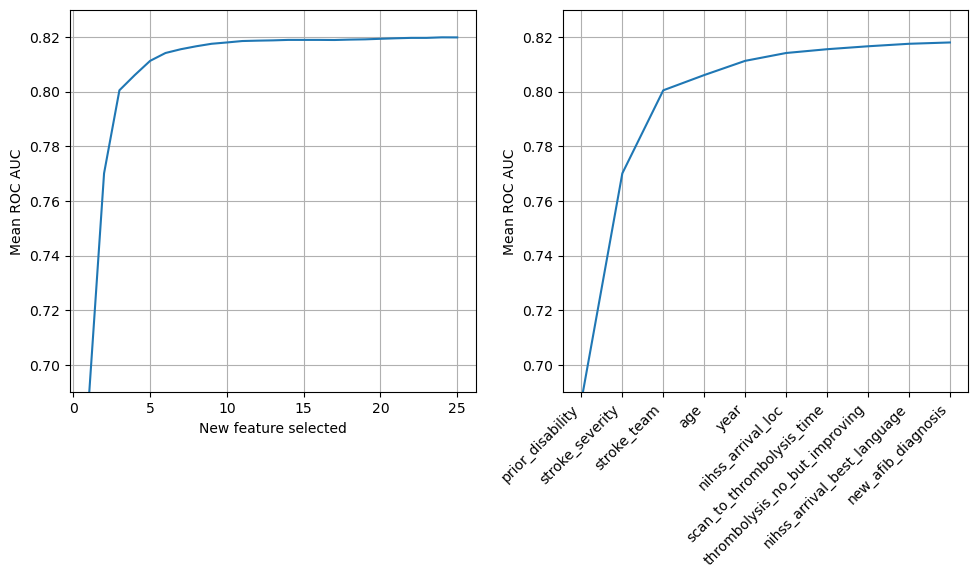
\includegraphics[width=0.75\textwidth]{./images/020_feature_selection.jpg}\\
    \caption{Feature selection}
    \label{fig:feature_selection}
\end{figure}

Figure \ref{fig:confusion_rocauc} shows the ROC-AUC results for the individual one vs one classes. There's is a better performance for classes to be distiguishable when they are further from each other in value. 

\begin{figure}[h!]
    \centering
    {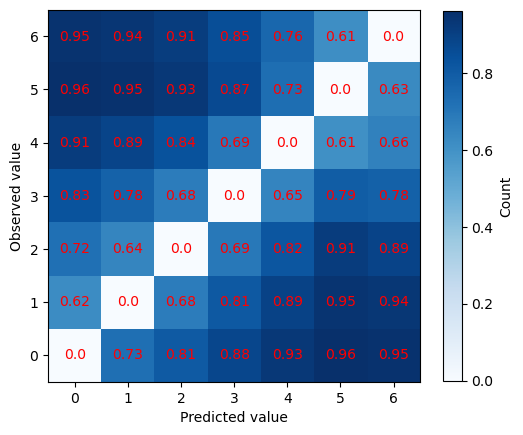
\includegraphics[width = 4in]{./images/040_ROCAUC_confusion_matrix_ovo.png}}\\
    \caption{ROC-AUC results for the individual one vs one classes}
    \label{fig:confusion_rocauc}
\end{figure}

Figure \ref{fig:confusion_mrs} shows the confusion matrices for the 5 kfolds. Given the consistency across the 5 kfolds, we will now only use results from the first kfold.
%040_confusion_matrices_5fold.png
\begin{figure}[!h]
    \centering
    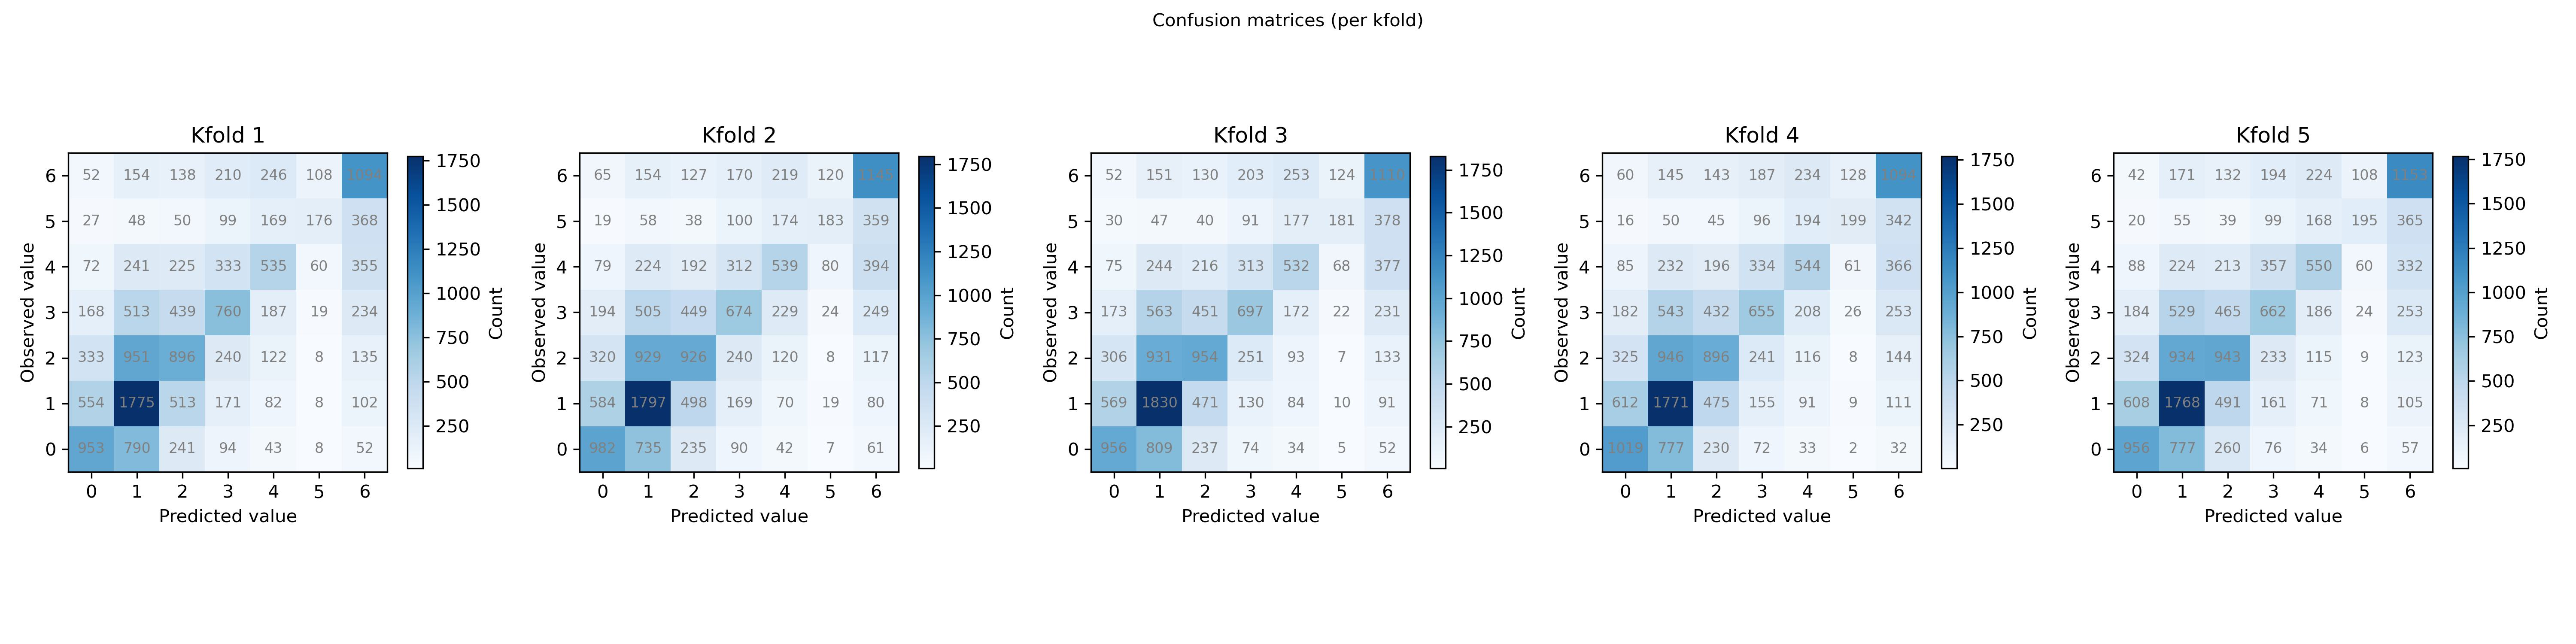
\includegraphics[width=1\textwidth]{./images/040_xgb_7_features_5fold_confusion_matrices_per_kfold.jpg}\\
    \caption{}
    \label{fig:confusion_mrs}
\end{figure}


Figure \ref{fig:violin_population_mRS} shows the outcome at population level for the different treatment scenarios.

\begin{figure}[!h]
    \centering
    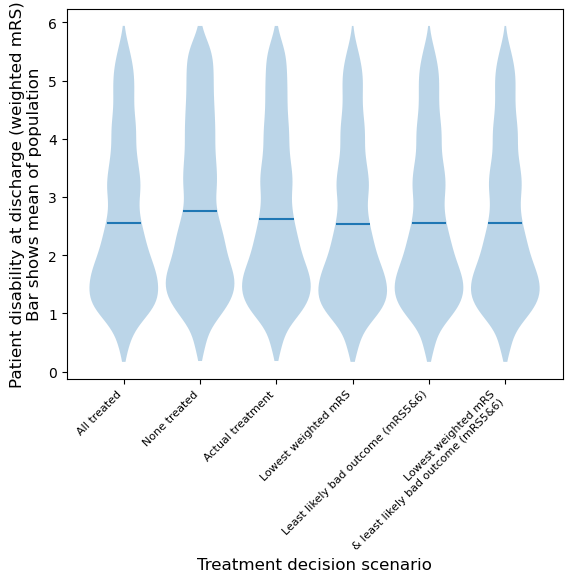
\includegraphics[width=0.7\textwidth]{./images/210_violin_population_weighted_mRS_per_treatment_scenario.png}\\
    \caption{Violin plot showing the population weighted mRS for each treatment scenario, with the bar showing the mean of the population.}
    \label{fig:violin_population_mRS}
\end{figure}


\subsection{\textit{Thrombolysis decision} model: Accuracy}

Figure \ref{fig:rocauc_thrombolysis_decision} shows the ROCAUC results for the two \textit{matching treatment} models. 


\begin{figure}
\centering
  \captionsetup{width=.9\linewidth}
  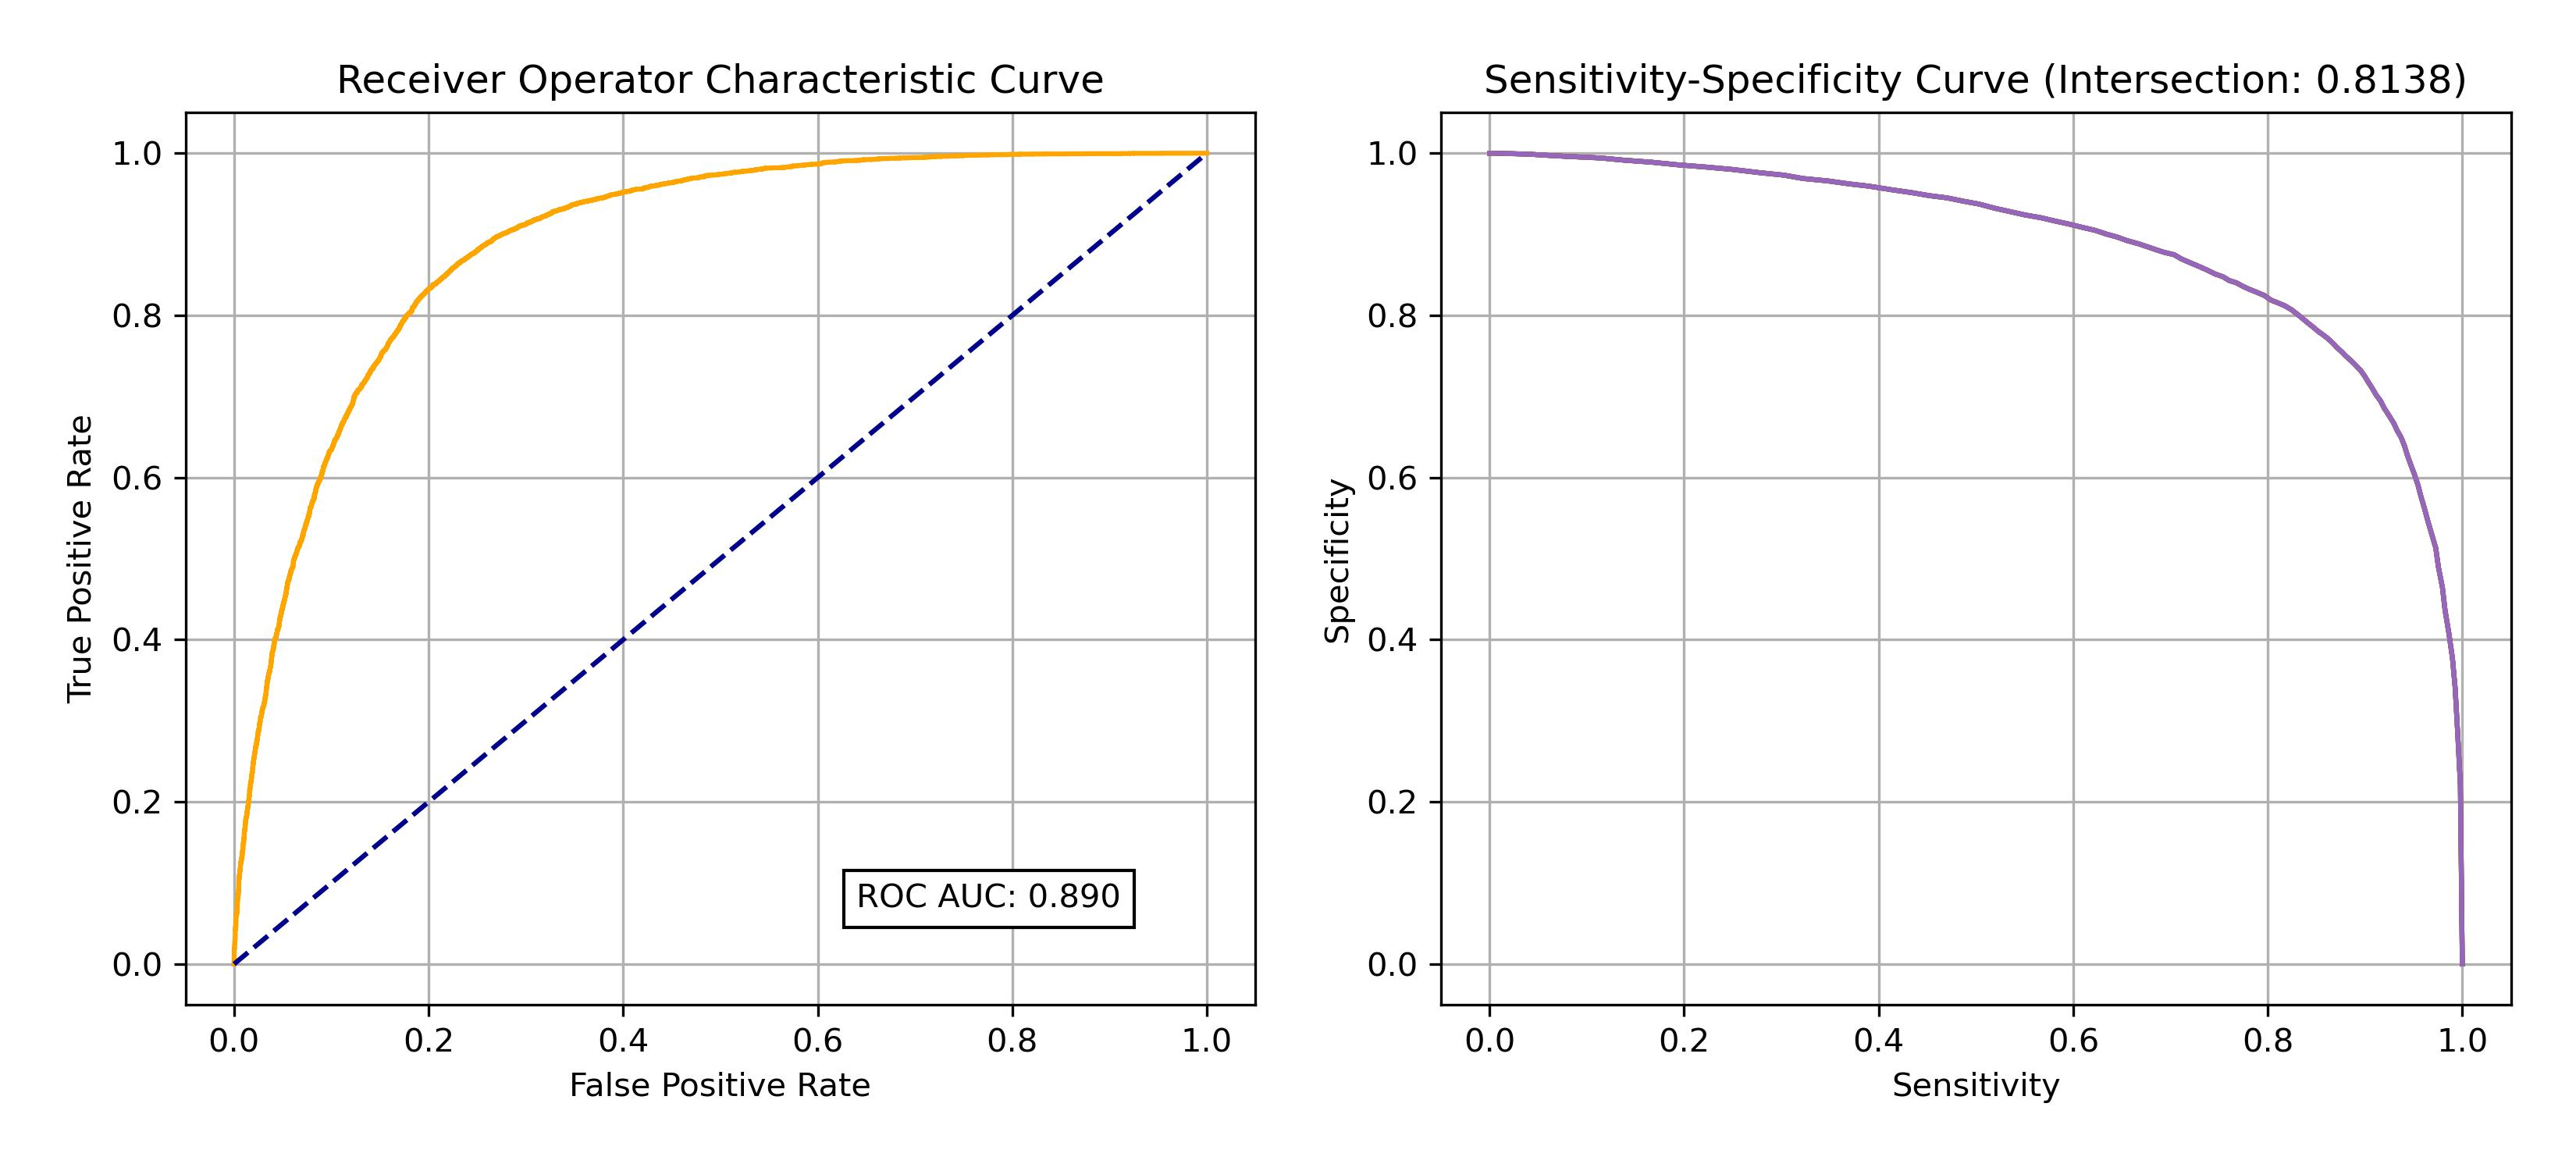
\includegraphics[width=1\textwidth]{./images/200_xgb_8_features_all_data_thrombolysis_decision_roc_sens_spec.jpg}\\
  \caption{Predicting patients receive thrombolysis (of those not have anticoagulants)}
  \label{fig:rocauc_thrombolysis_decision}
\end{figure}


\iffalse
\begin{figure}
\centering
  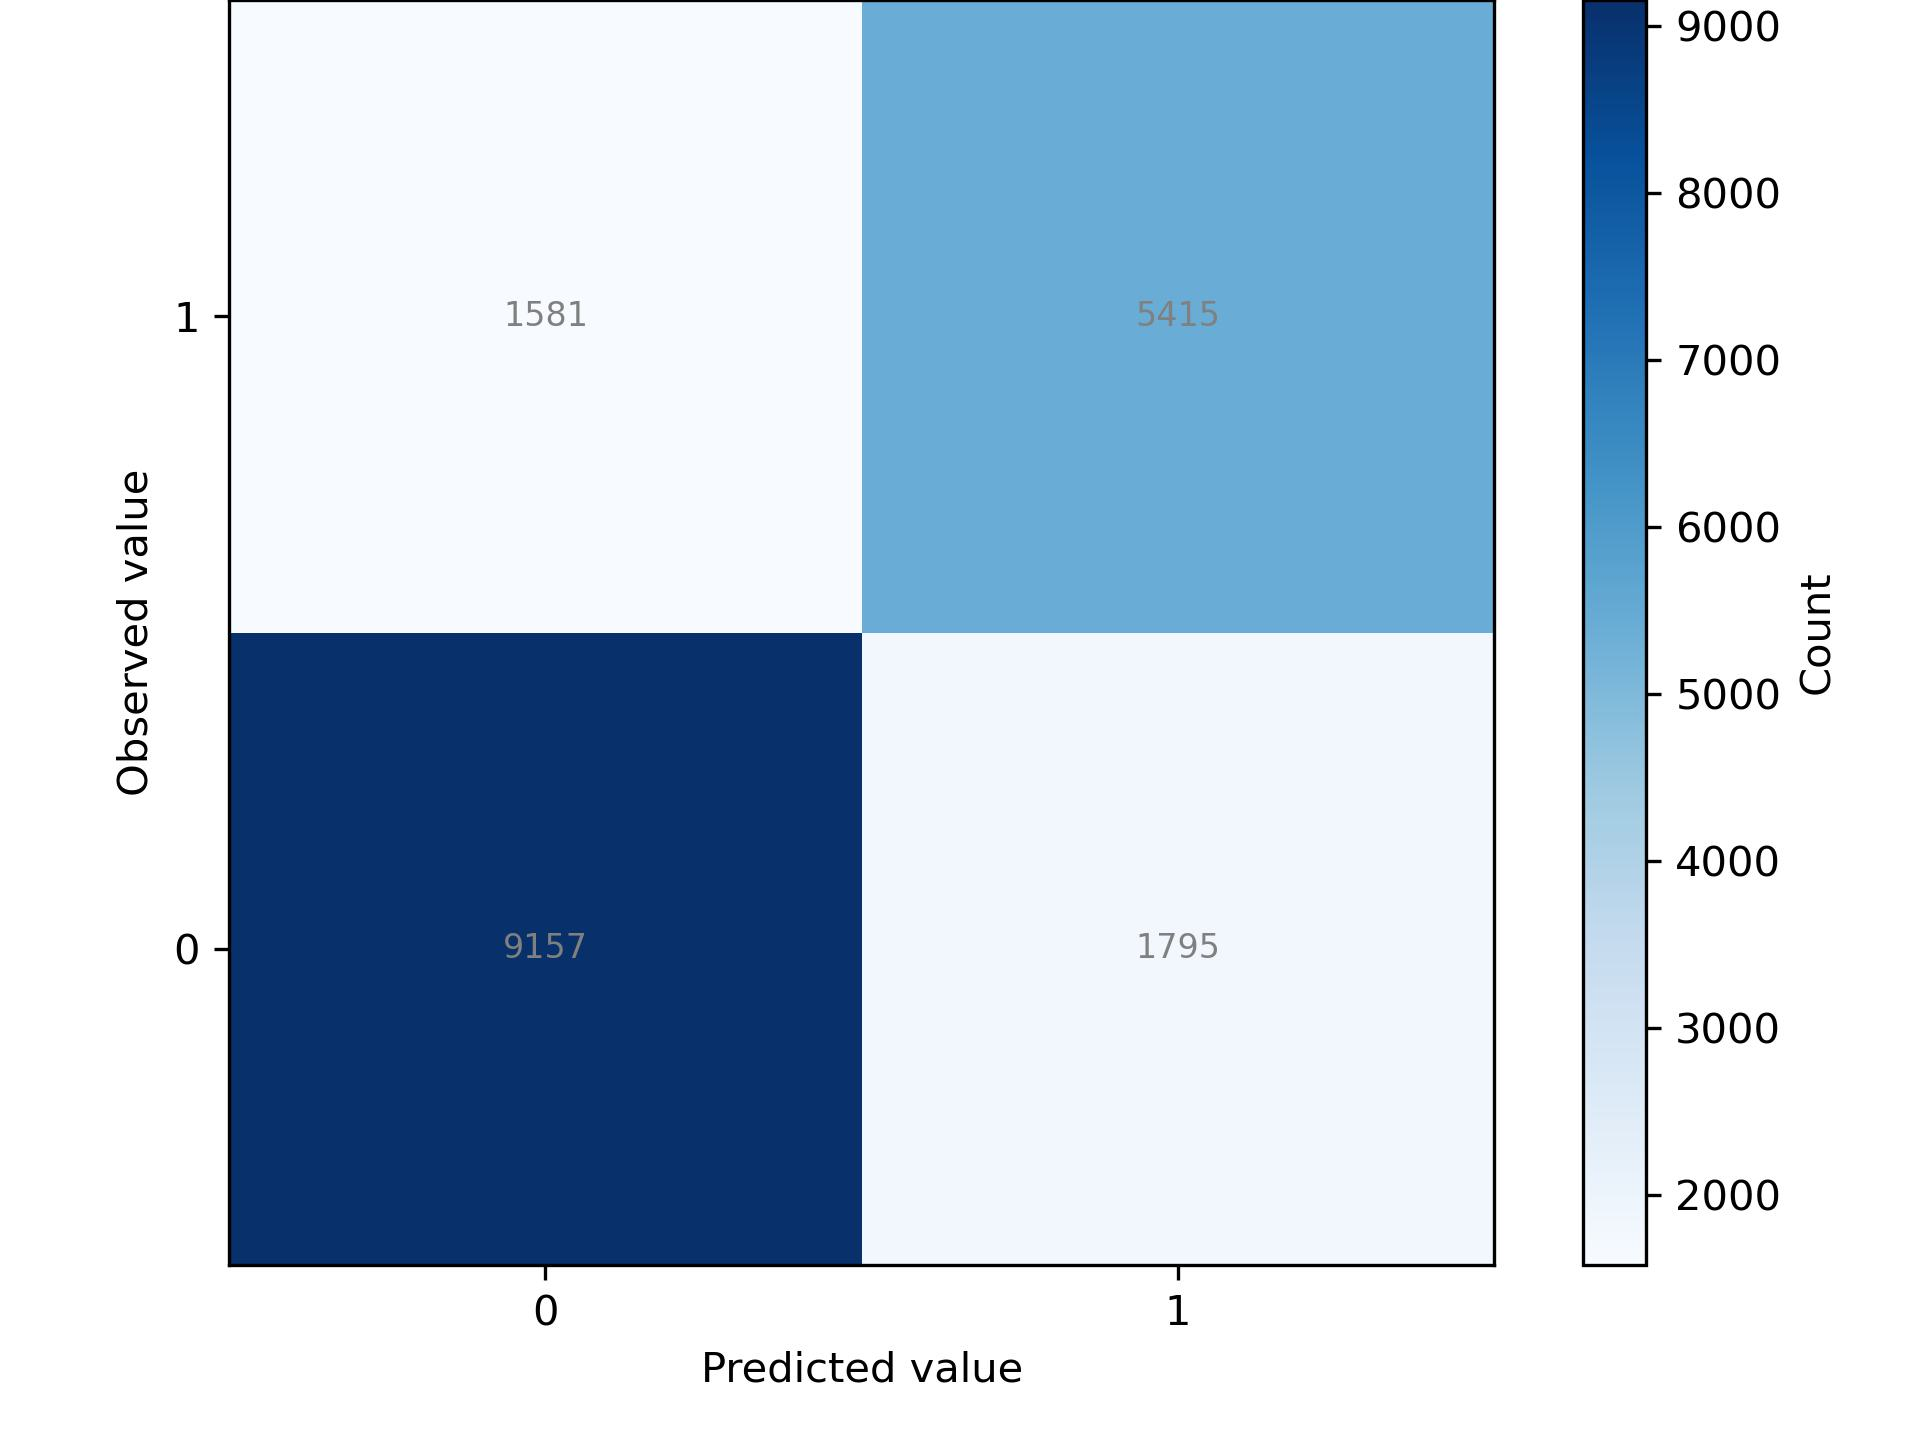
\includegraphics[width=0.6\textwidth]{./images/200_xgb_8_features_all_data_thrombolysis_decision_confusion_matrix}\\
  \caption{Predicting had treatment for those predicted to have better outcome from treatment}
  \label{fig:cm_thrombolysis_decision}
\end{figure}



\textbf{Violin plots}
Illustrate this with a violin plot. Figure \ref{fig:shap_violin_all_benefit_ivt} shows patients who should benefit from treatment. What is it about the patients that means they didn't receive it, but would have benefited from treatment?

\begin{figure}
\subfloat[]{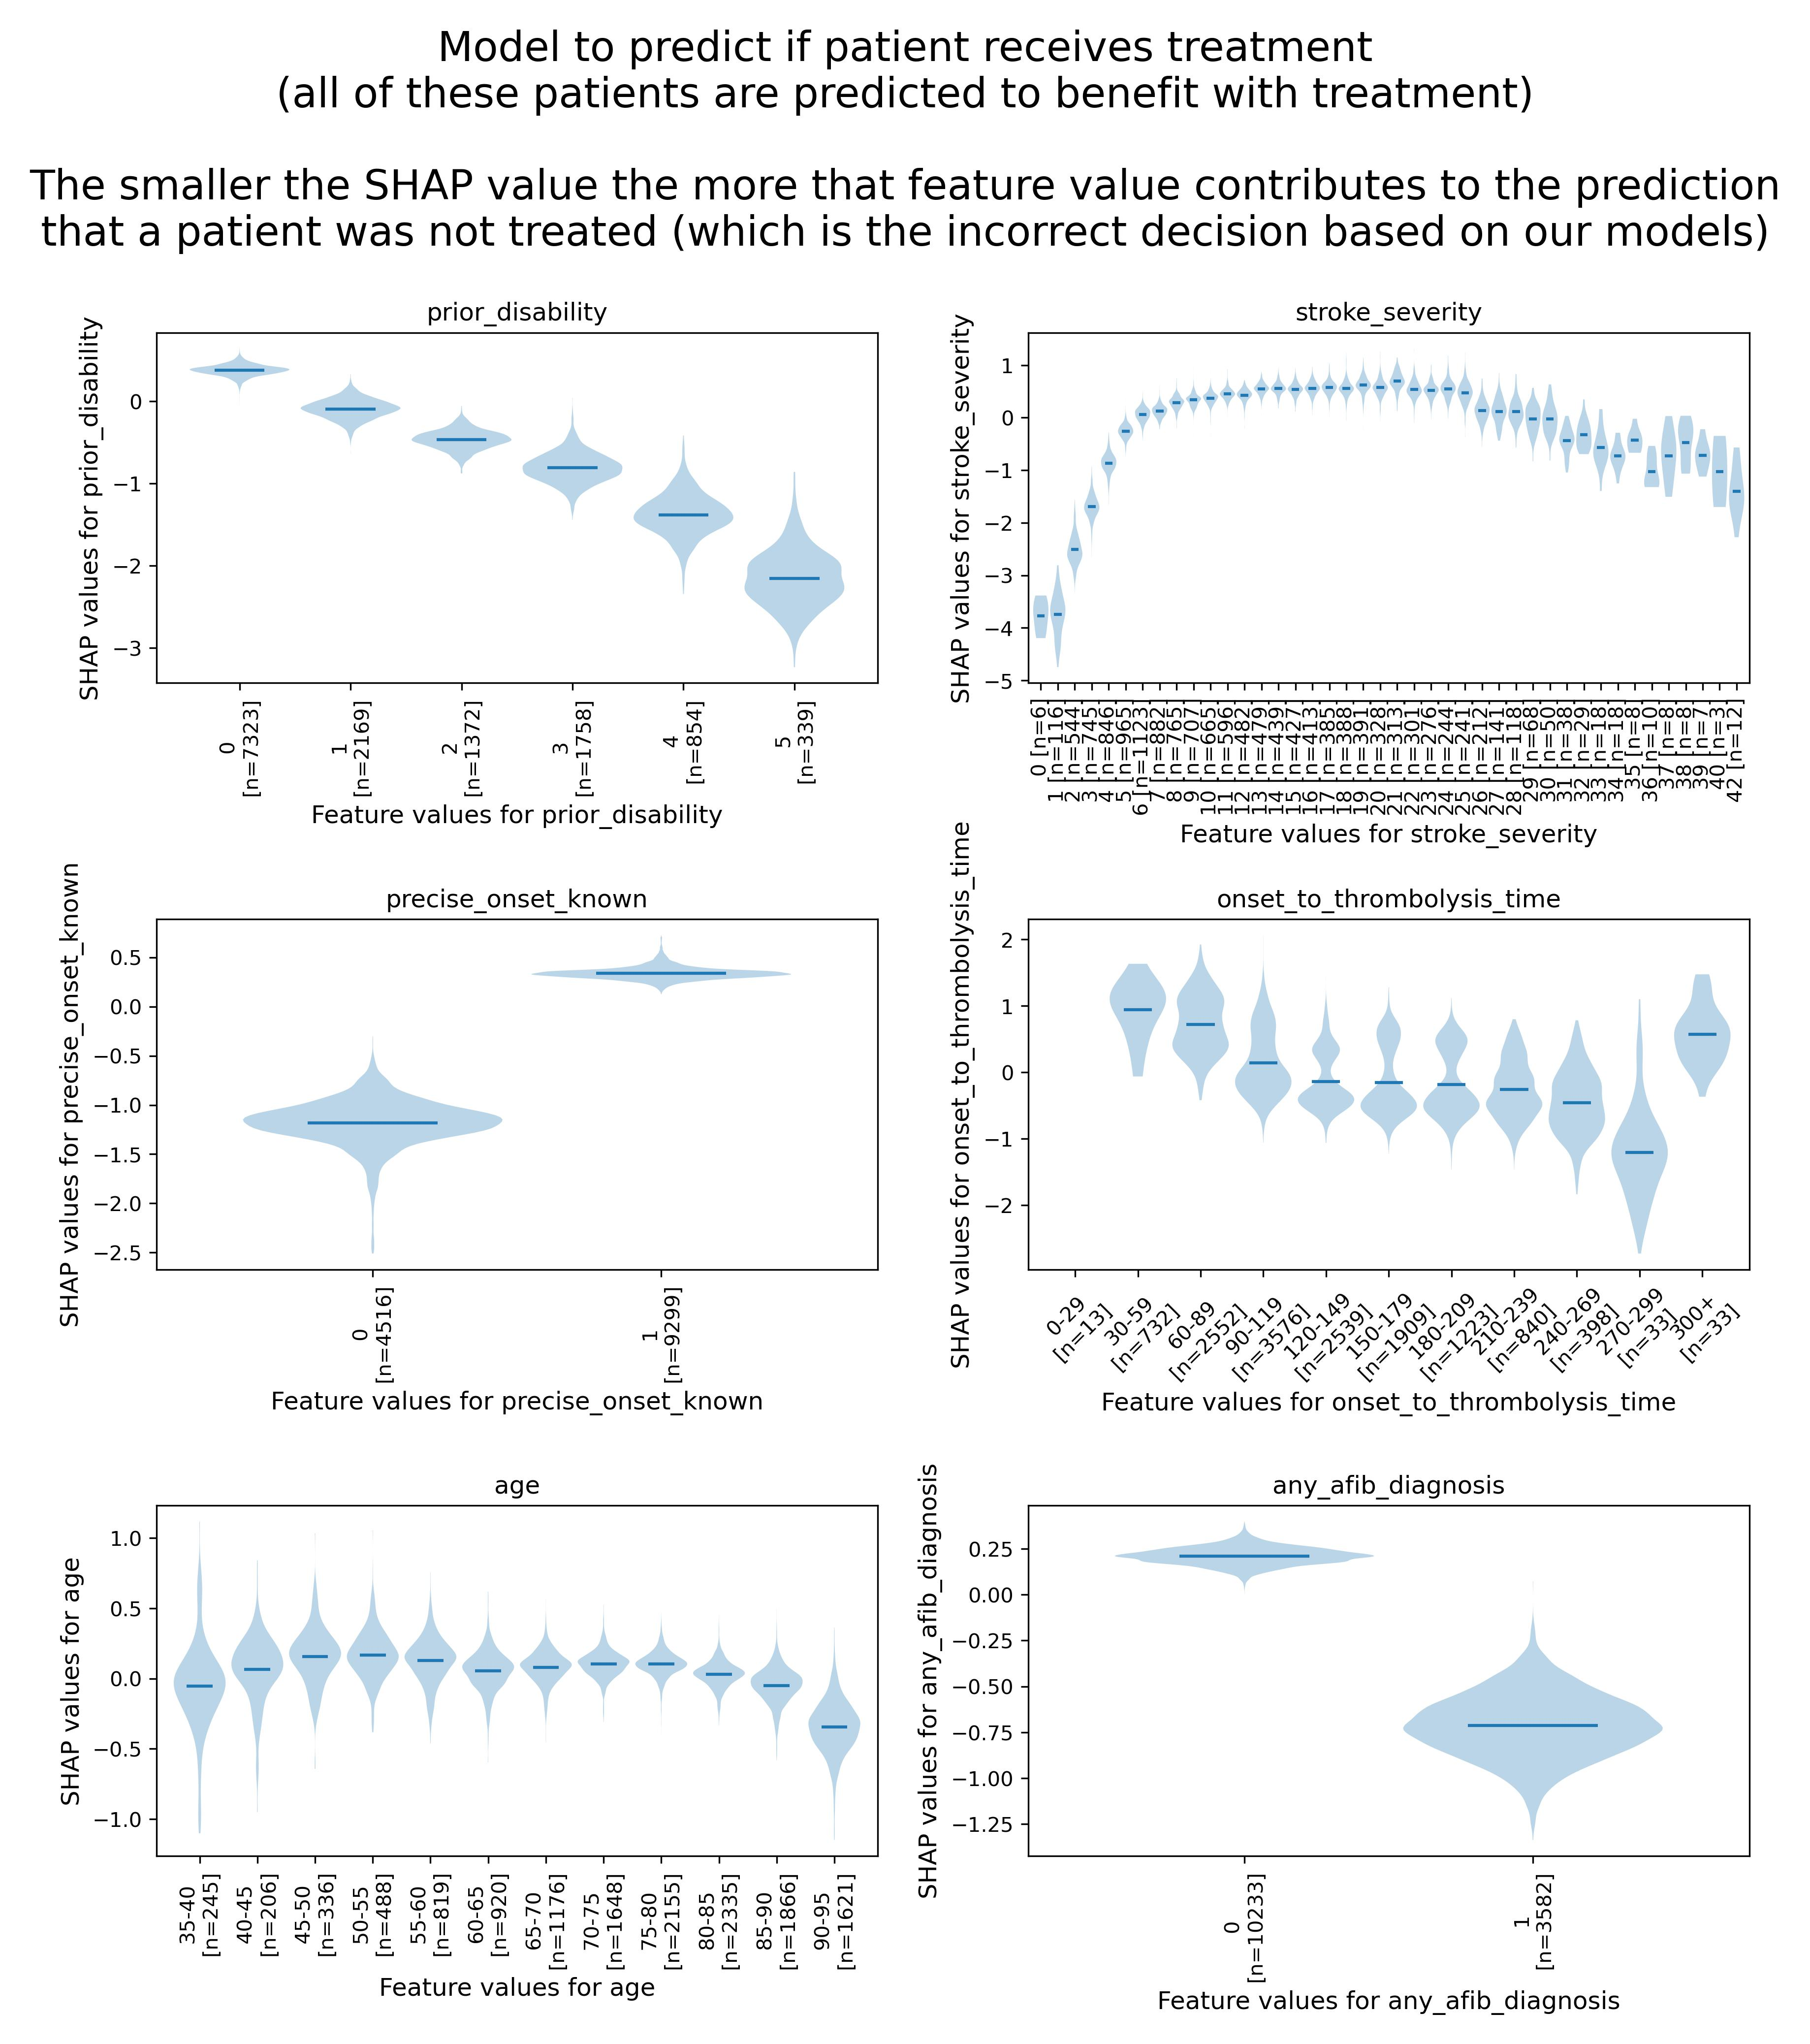
\includegraphics[width = 5in]{./images/218_shap_violin_all_benefit_with_ivt_Lowest_weighted_mrs_and_least_mrs5_6_Actual_treatment.jpg}}\\
\caption{}
\label{fig:shap_violin_all_benefit_ivt}
\end{figure}

\ref{fig:shap_violin_none_benefit_ivt} shows patients who should not benefit from treatment. What is it about the patients that means they received it, but would have benefited from not receiving treatment?

\begin{figure}
\subfloat[]{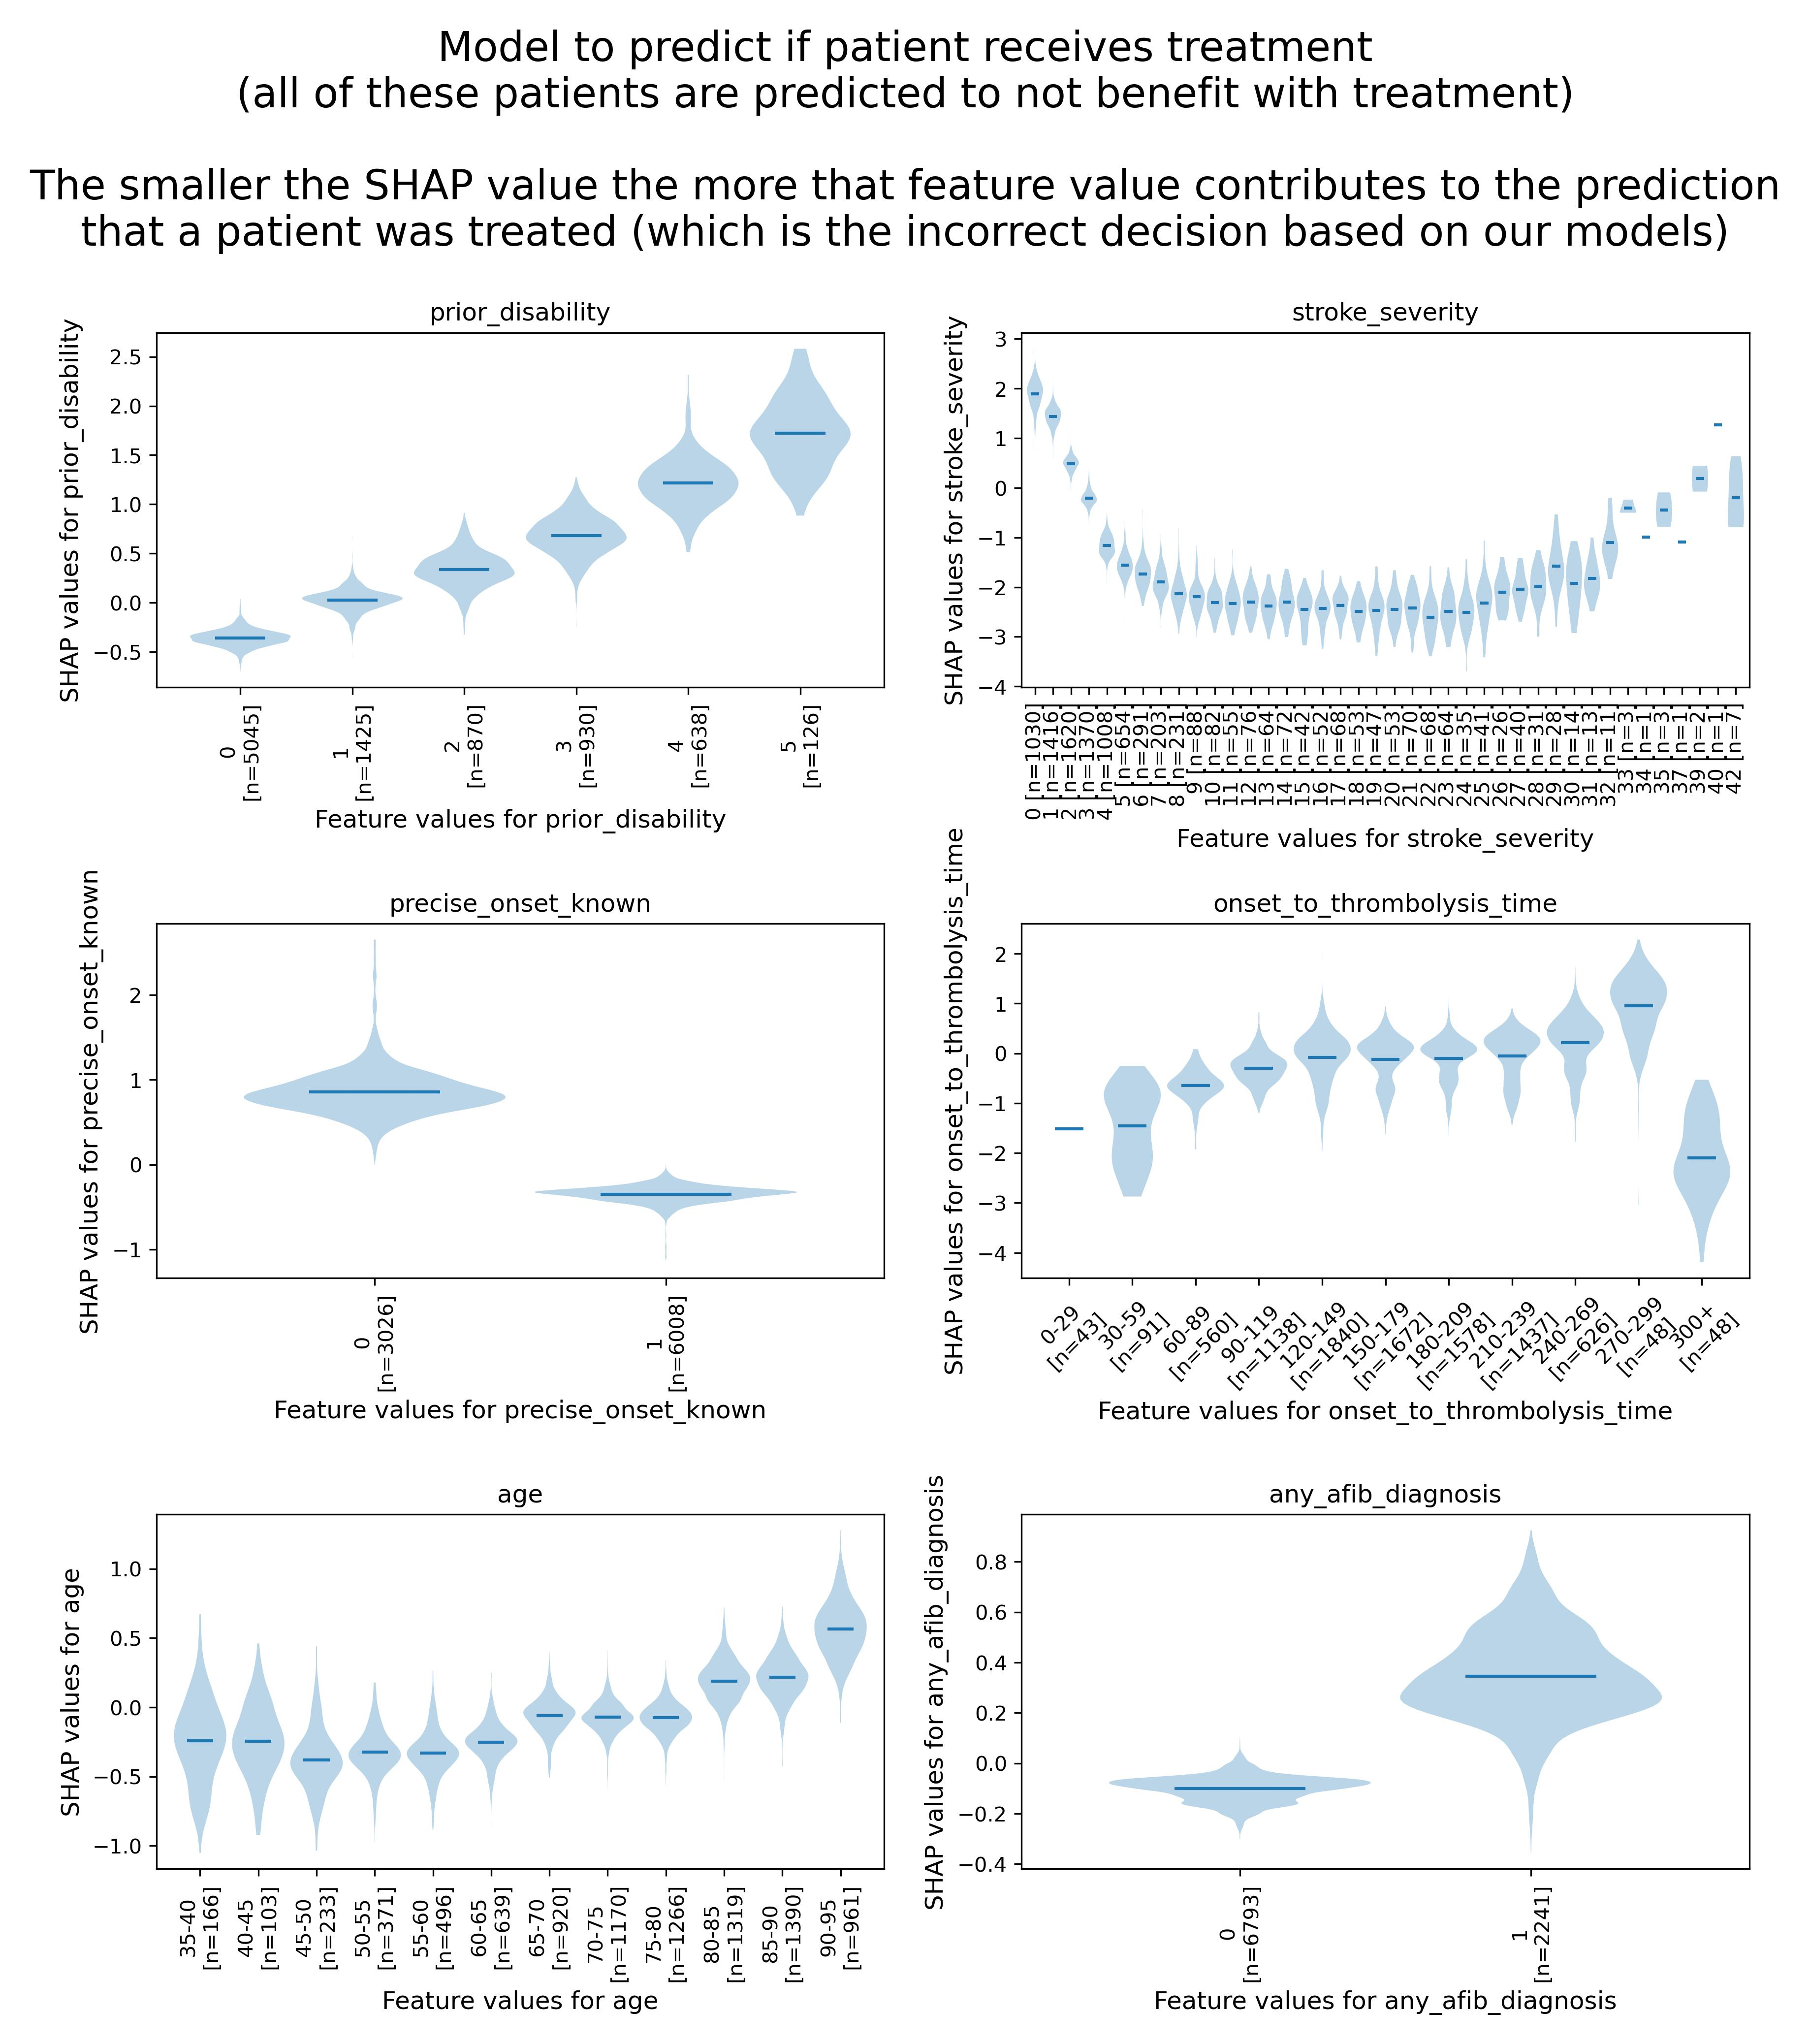
\includegraphics[width = 5in]{./images/218_shap_violin_none_benefit_with_ivt_Lowest_weighted_mrs_and_least_mrs5_6_Actual_treatment.jpg}}\\
\caption{}
\label{fig:shap_violin_none_benefit_ivt}
\end{figure}

See the points as relative, as zero means it is not shifting model from base SHAP.

Safest bet of the best outcome with treatment, choose a patient with ideal characteristics (these are younger, no AF, early IVT, SS 10-25).

These ideal characteristic values also identify patients that have been given thrombolysis but are predicted to not have the best outcome with treatment. So we can't say always give it to a single certain characteristic value, as need to take into account all characteristics.

So a drug label contains a list of ideal characteristics - if you follow this then you miss benefit. 

In order to recognise those patients who would, and would not, you need a model to combine all the characteristics. It's combination of characteristics, not a single value. No simple rules to recognise patients who should be treated but aren't currently receiving treatment (and vice versa).

On the flip side, non-ideal characteristic values (such as older, AF, later IVT, SS mild or severe) help to identify patients that have not been given thrombolysis but are predicted to have the best outcome with treatment.

All of this points back to needing a model.

The model takes into account prior disability 
\fi

% Word counts - Don't count these!
%TC:ignore
%\section*{Word counts}
%\detailtexcount{main}
%TC:endignore

\end{document}